\newpage
\section{实验}
\label{sec:experiment}

\subsection{数据准备}
为了更好地开展商品信息相关的实验、测试,现以Product-10K数据集\cite{bai2020products10k}中的商品图片为基础,利用本地部署的多模态LLM批量生成这些商品对应的商品信息,再将这些信息输入到中心服务器中,以达到替代实际商品商品信息的目的。该数据集中的图片以存货单位(SKU)、商品类别为分类方式。在本实验中属于同一SKU的图片将被视为同一个商品的图片,每个SKU都会被随机挑出一个图片作为其代表交由LLM进行处理。文字部分利用的LLM是30亿参数版本 \verb|qwen2.5| 。

本实验利用本地部署的80亿参数版本 \verb|minicpm-v| 大模型进行商品图像描述的编写,使用的提示词对话如下:

\begin{itemize}
    \item[] \textbf{用户:}
    \begin{itemize}
        \item[] \textbf{(商品图片数据)}
        \item[] \textbf{(文字消息)} 细致地描述这个图片中的内容,以便其他模型利用这段描述进行进一步推理。
    \end{itemize}
\end{itemize}

然而,对生成结果(及其对应图片)的人工抽查显示数据集中某些图片更加接近生活照片,难以被断定为商品图片。因此,以下的提示词对话被用于检测图片是否代表一个商品:

\begin{itemize}
    \item[] \textbf{用户:} 以下是从一个图片产生的说明,请根据这段说明判断该图片是否表示一个商品(布尔值字段verdict):\textit{(商品图片描述)}
\end{itemize}

以上提示词在使用的时候加入了对模型输出的限制(具有布尔值字段 \verb|verdict| 的JSON对象)。经过筛选之后的商品图片描述其后进入商品描述生成的过程:

\begin{itemize}
    \item[] \textbf{用户:} 请编写商品描述,商品描述应该尽可能有吸引力,并且不要输出商品描述之外的内容。以下是商品对应图片的描述:\textit{(商品图片描述)}
\end{itemize}

最后,生成的商品描述被用于进一步生成商品标题:

\begin{itemize}
    \item[] \textbf{用户:} 为这段商品介绍产生一个言简意赅的商品标题:\textit{(商品描述)}
\end{itemize}

生成的商品标题、描述等数据其后被收集起来,并且与其图片相绑定。之后,这些数据被通过第 \ref{sec:foundation} 部分提及的服务器API传输到数据库中,用于后续试验。

\subsection{服务端}

\subsubsection{RmInit}

% \begin{figure}[htbp]
% 	\centering
% 	\includegraphics[width=0.8\textwidth]{./exp/}
% 	\caption{(todo)}
% 	\label{fig:}
% \end{figure}

\begin{figure}[htbp]
    \subfloat{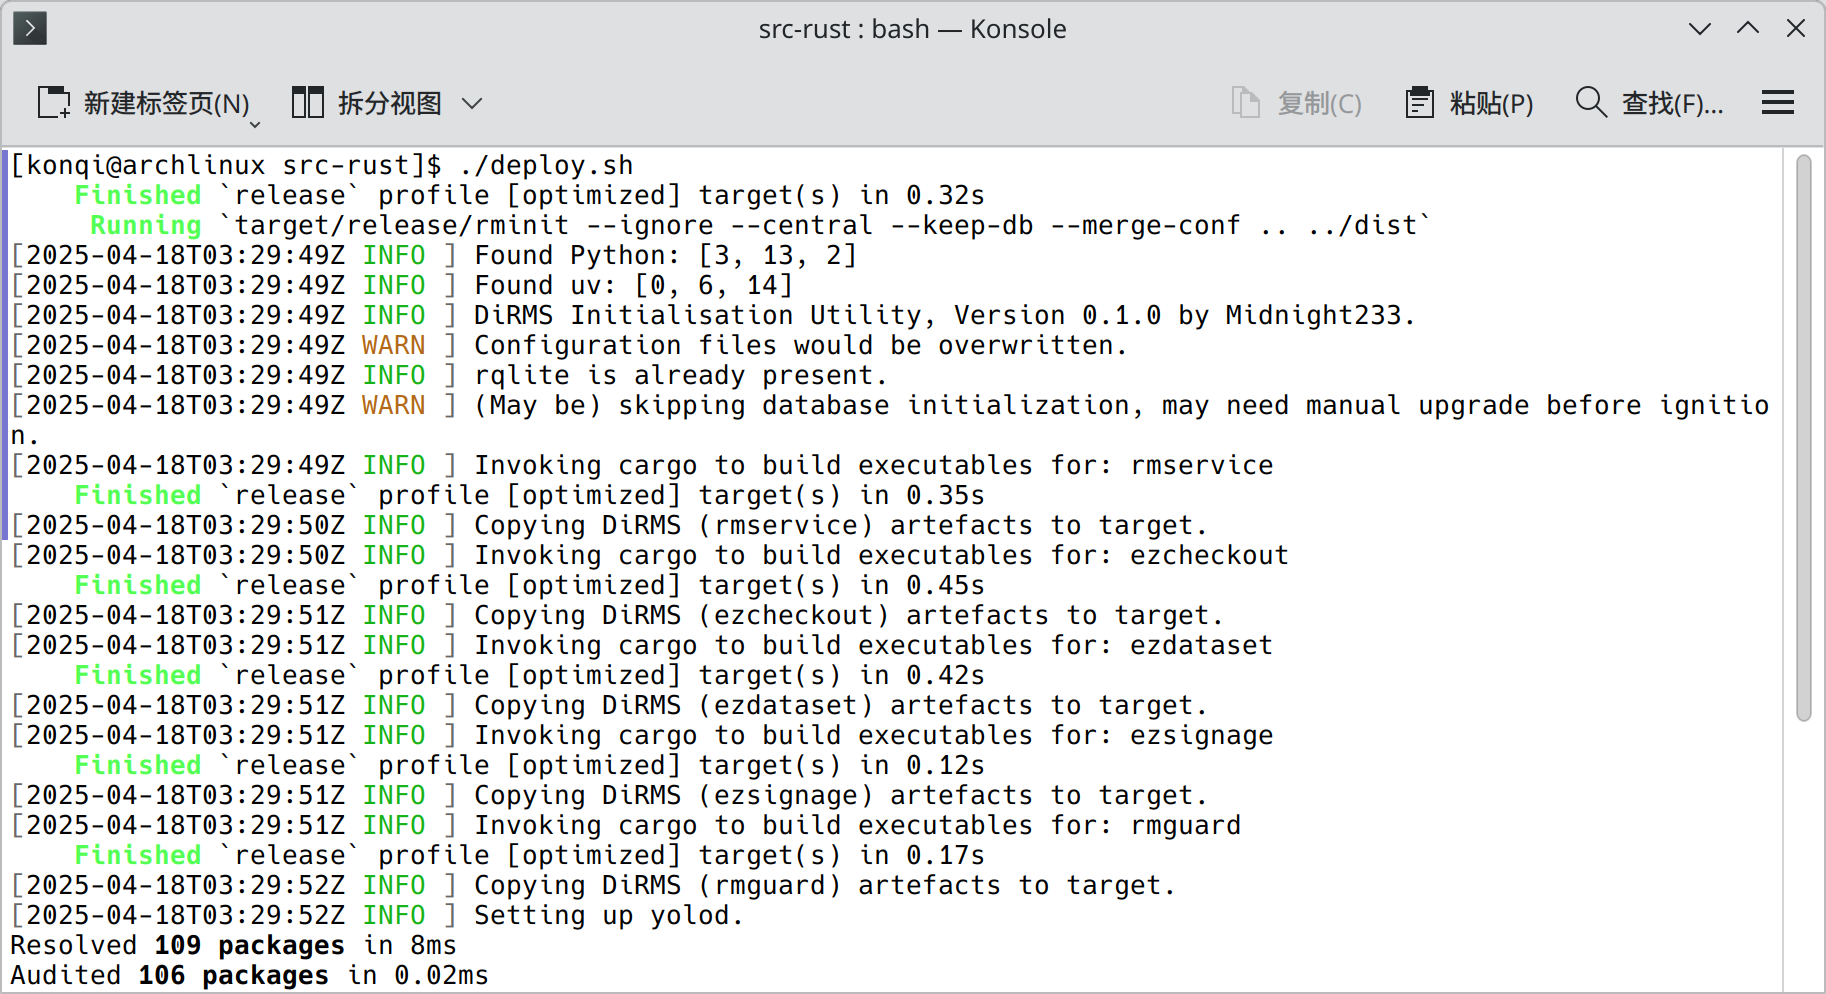
\includegraphics[width=0.45\textwidth]{./exp/rminit-1.png}}
    \hfill
    \subfloat{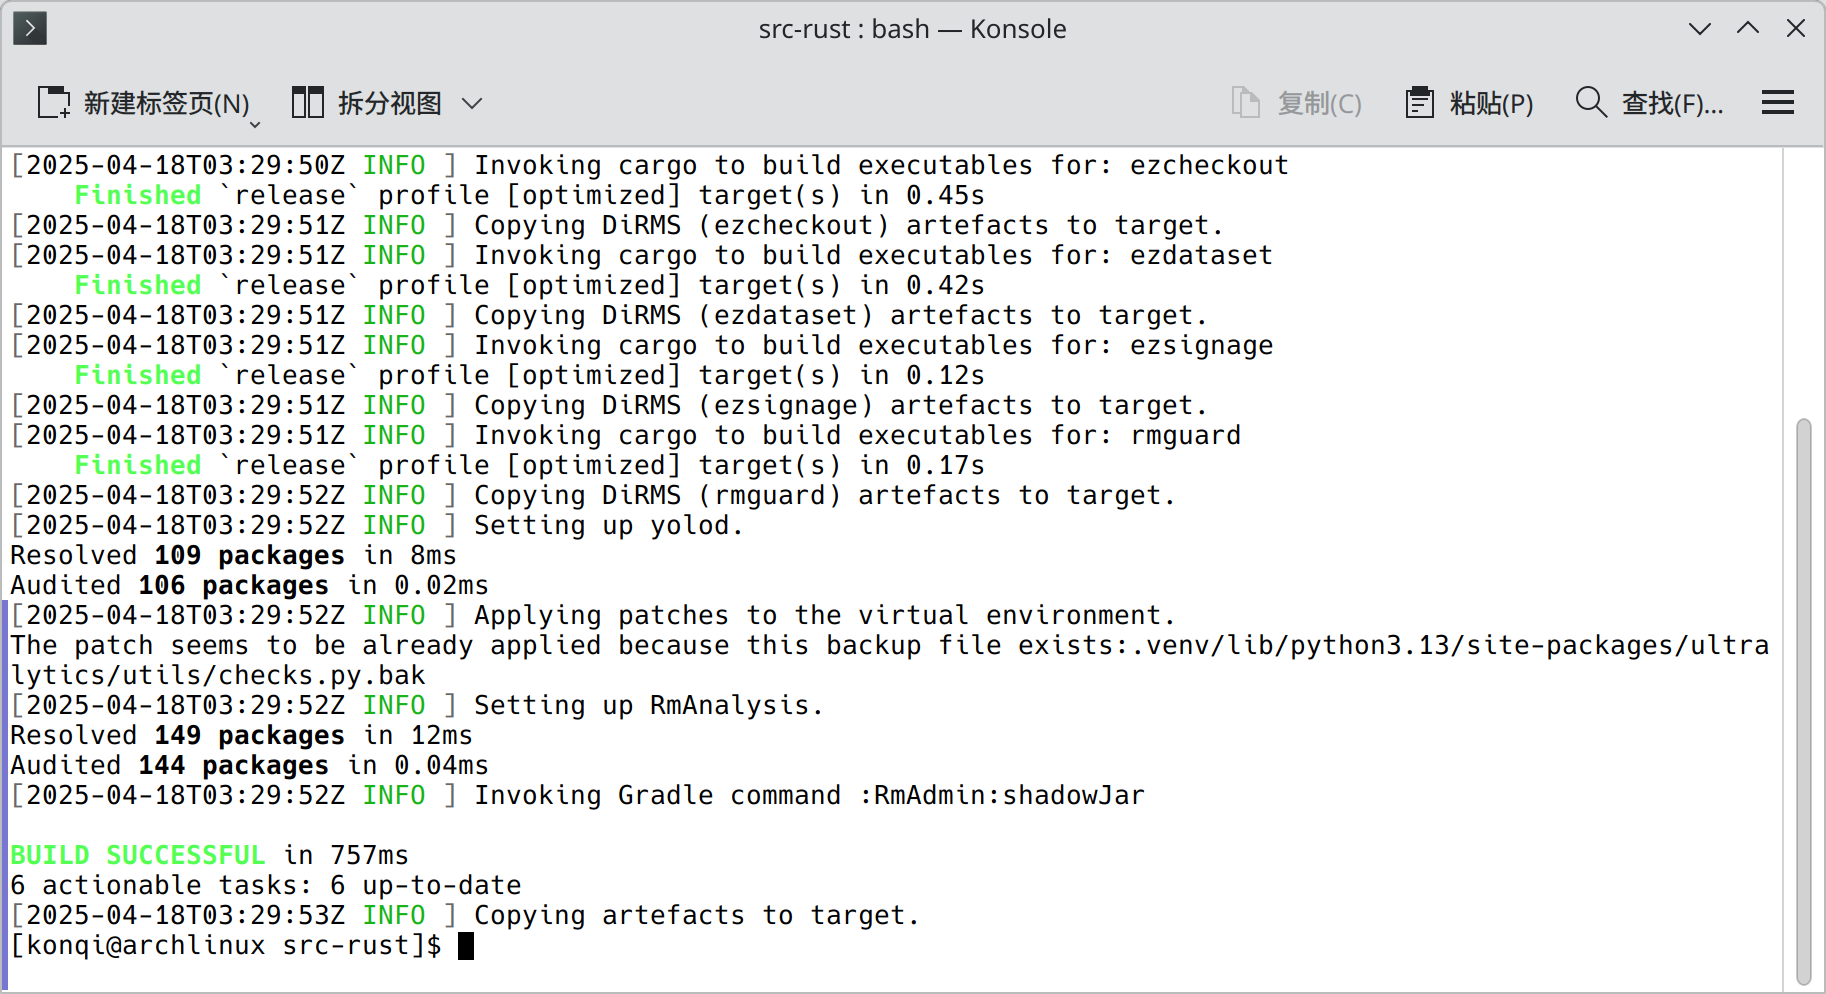
\includegraphics[width=0.45\textwidth]{./exp/rminit-2.png}}
	\caption{(todo)}
	\label{fig:rminit}
\end{figure}

\subsubsection{RmGuard}

\begin{figure}[htbp]
	\centering
	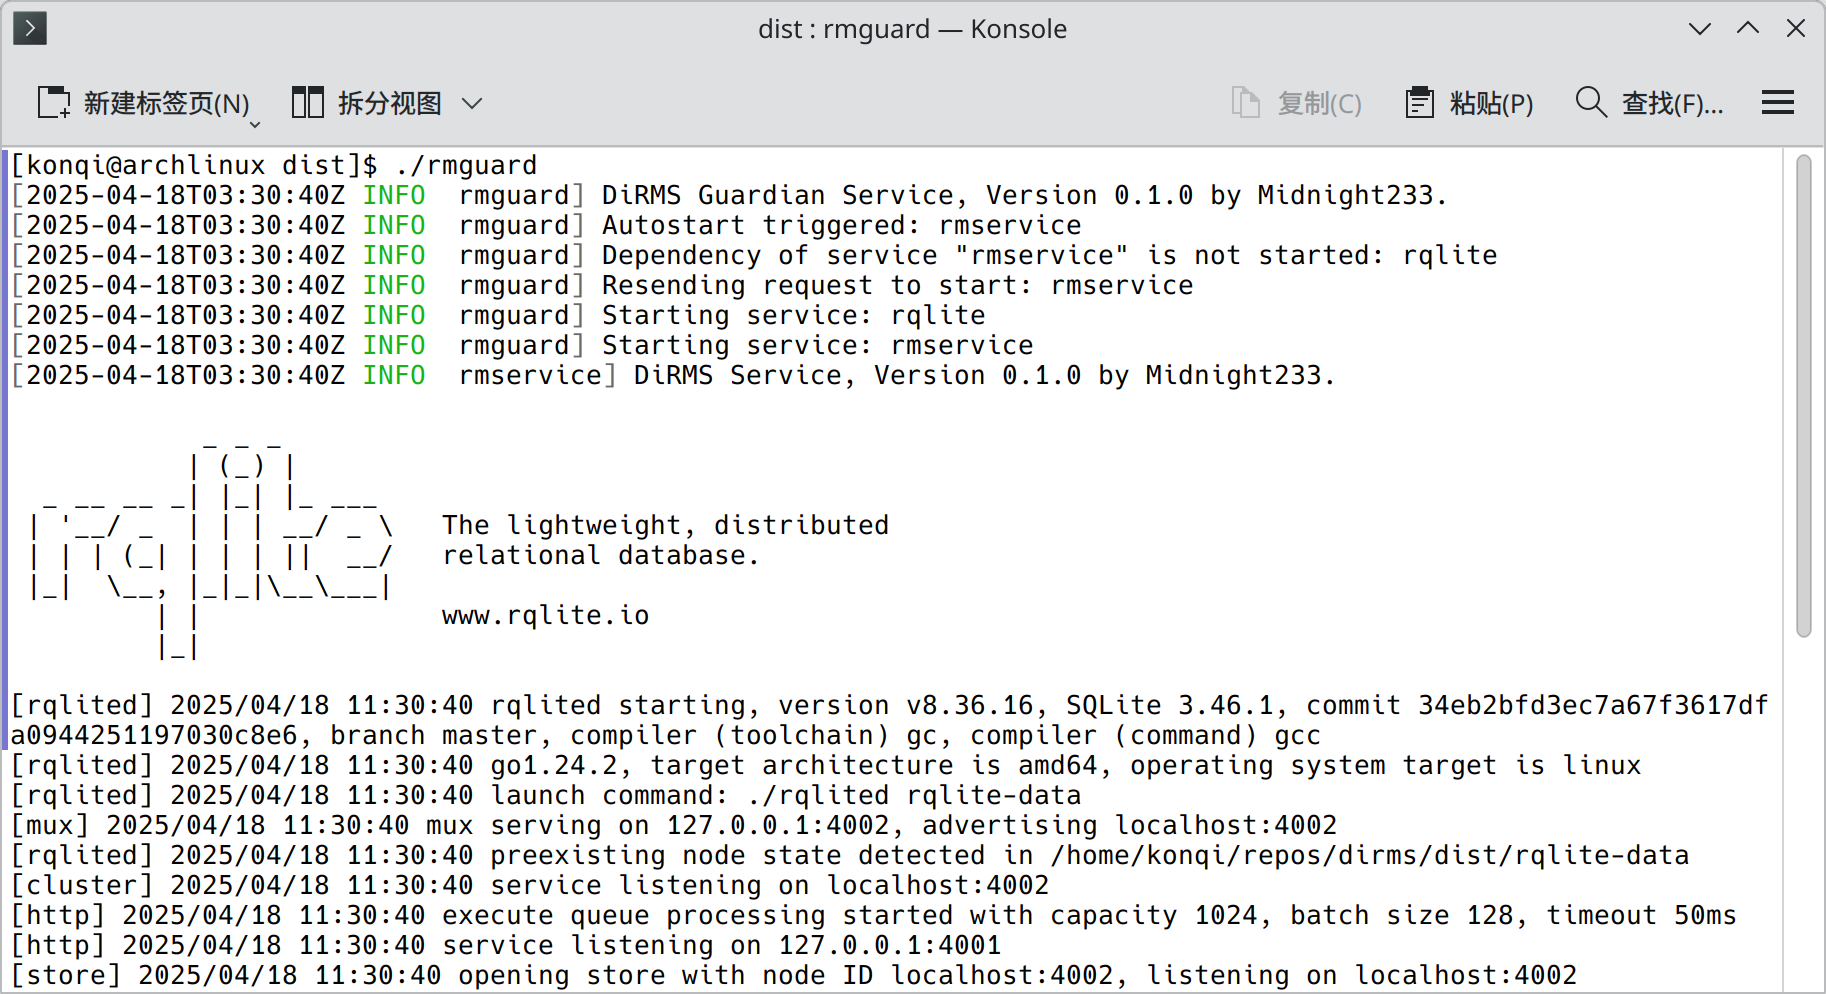
\includegraphics[width=0.8\textwidth]{./exp/rmg-core.png}
	\caption{(todo)}
	\label{fig:rmg-core}
\end{figure}

\begin{figure}[htbp]
    \subfloat{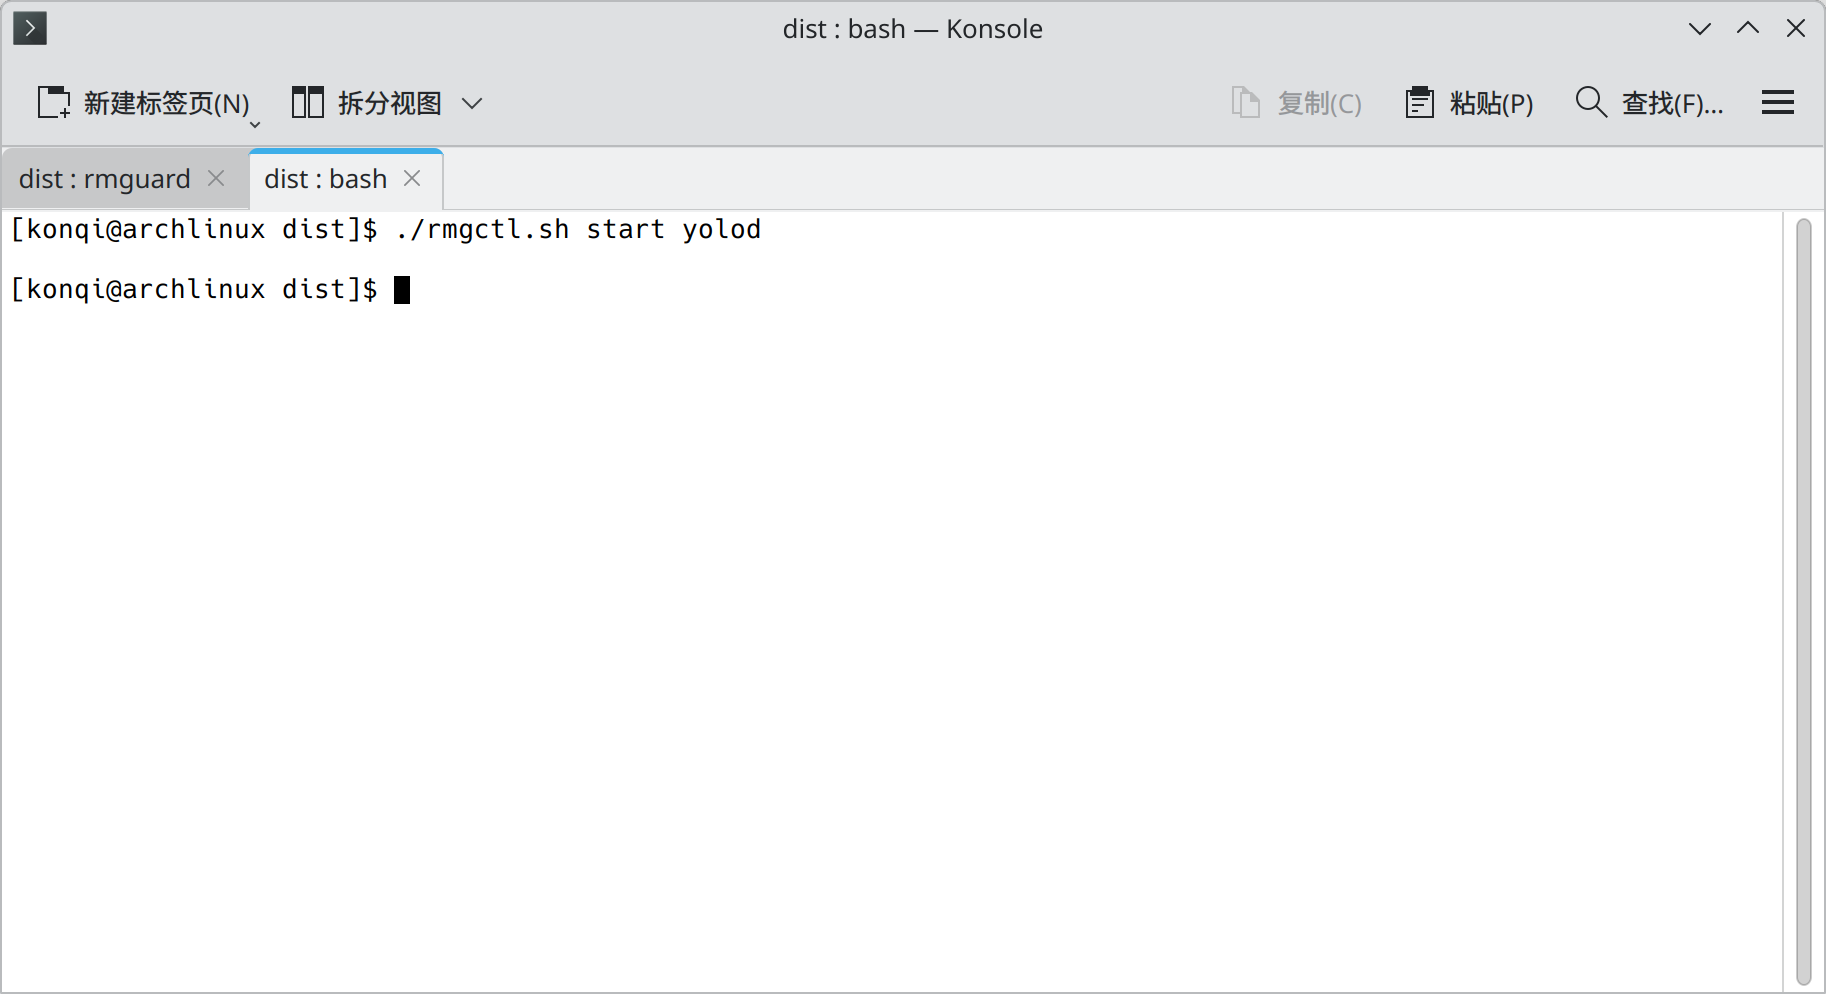
\includegraphics[width=0.45\textwidth]{./exp/rmg-yolod-1.png}}
    \hfill
    \subfloat{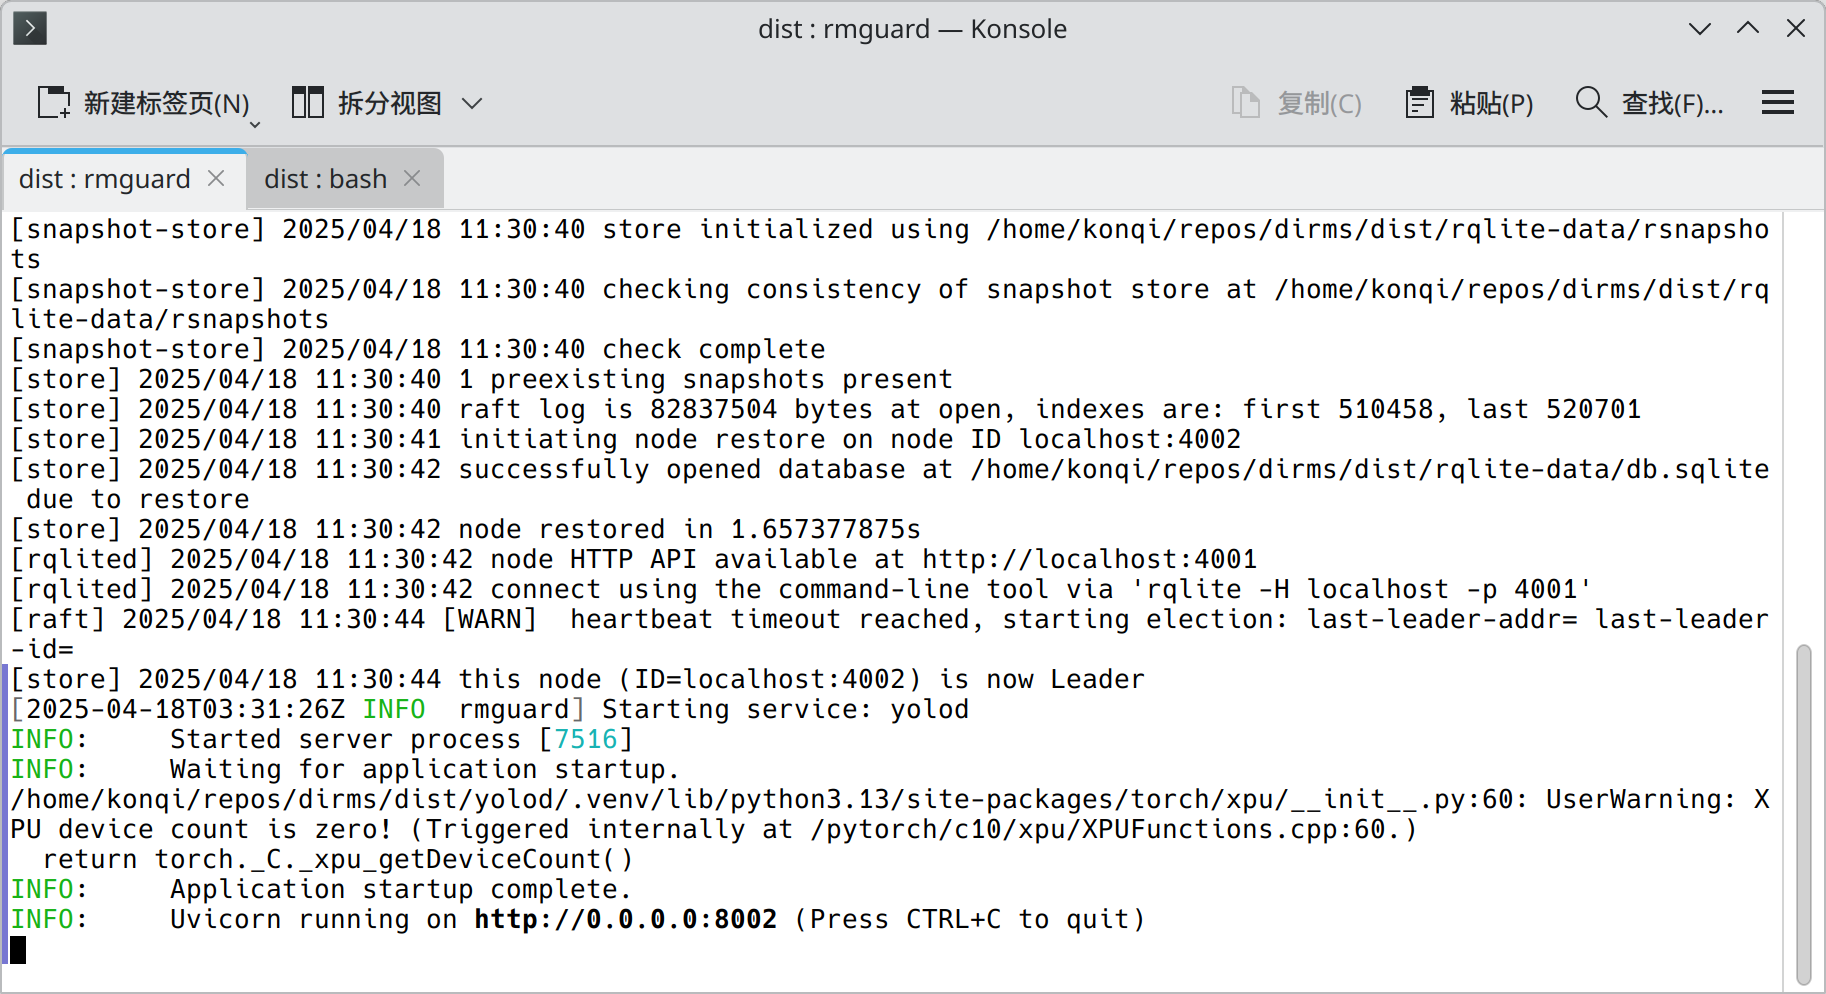
\includegraphics[width=0.45\textwidth]{./exp/rmg-yolod-2.png}}
    \vspace{1em}
    \subfloat{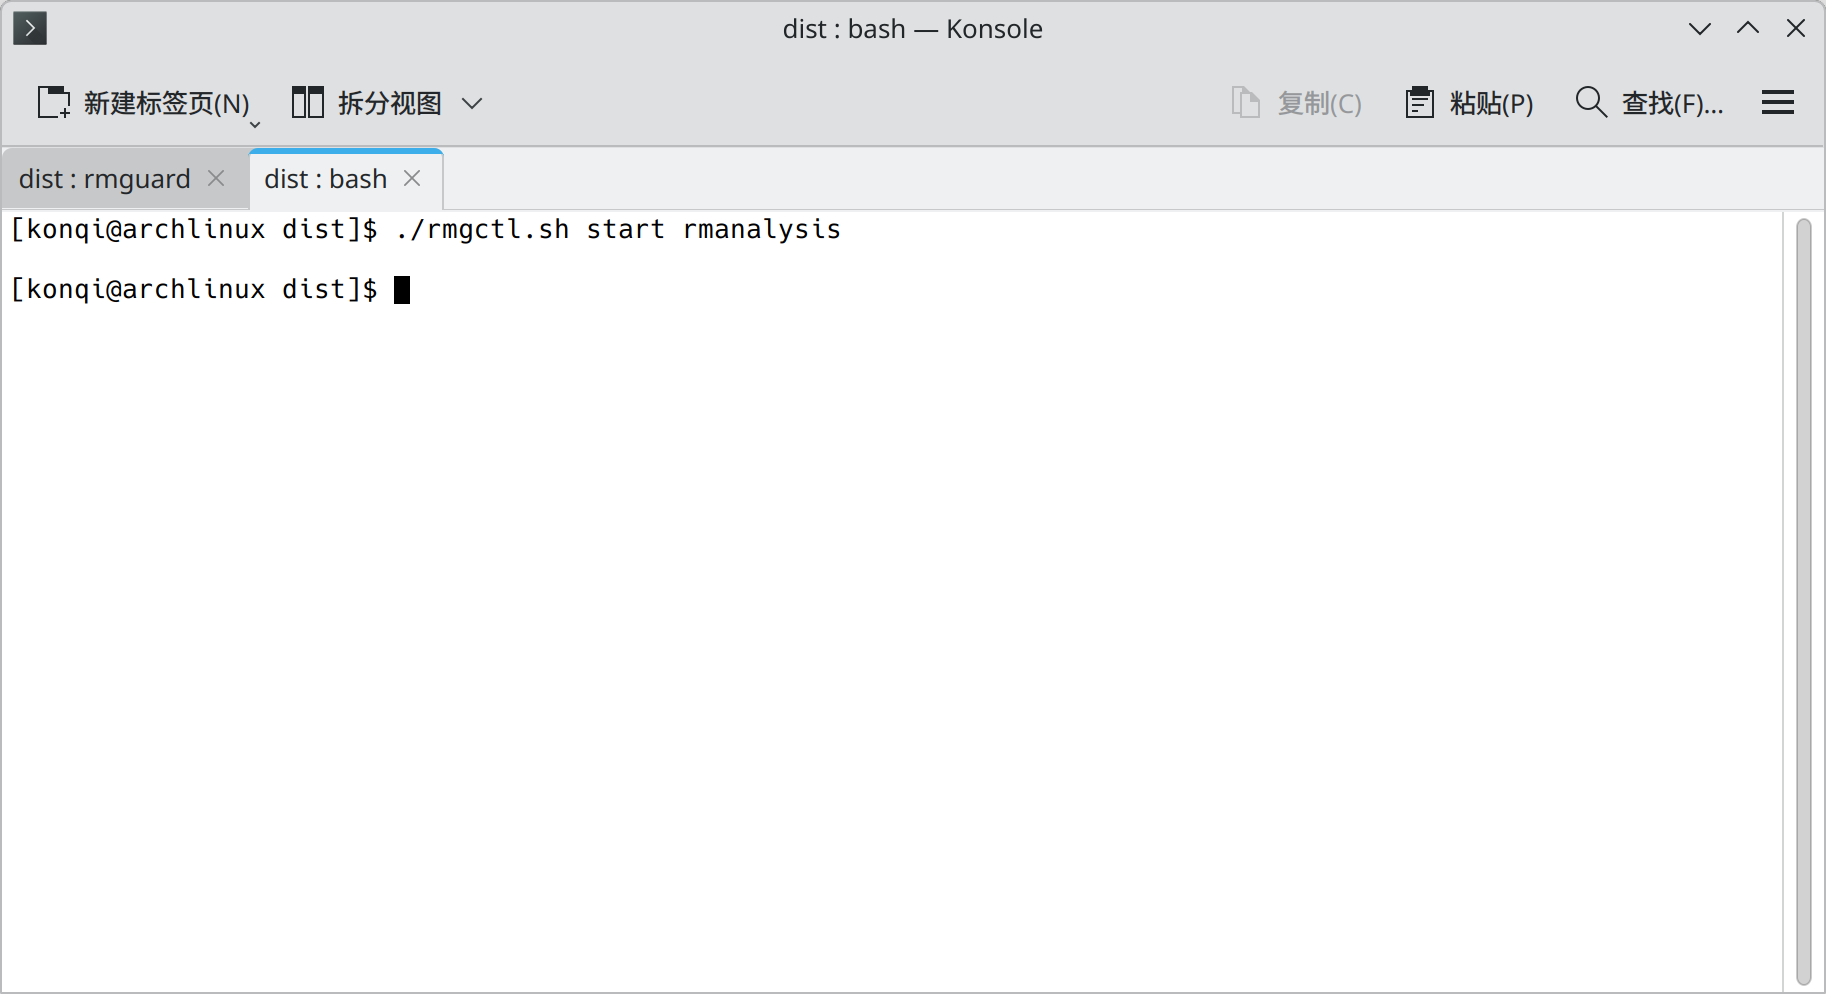
\includegraphics[width=0.45\textwidth]{./exp/rmg-rma-1.png}}
    \hfill
    \subfloat{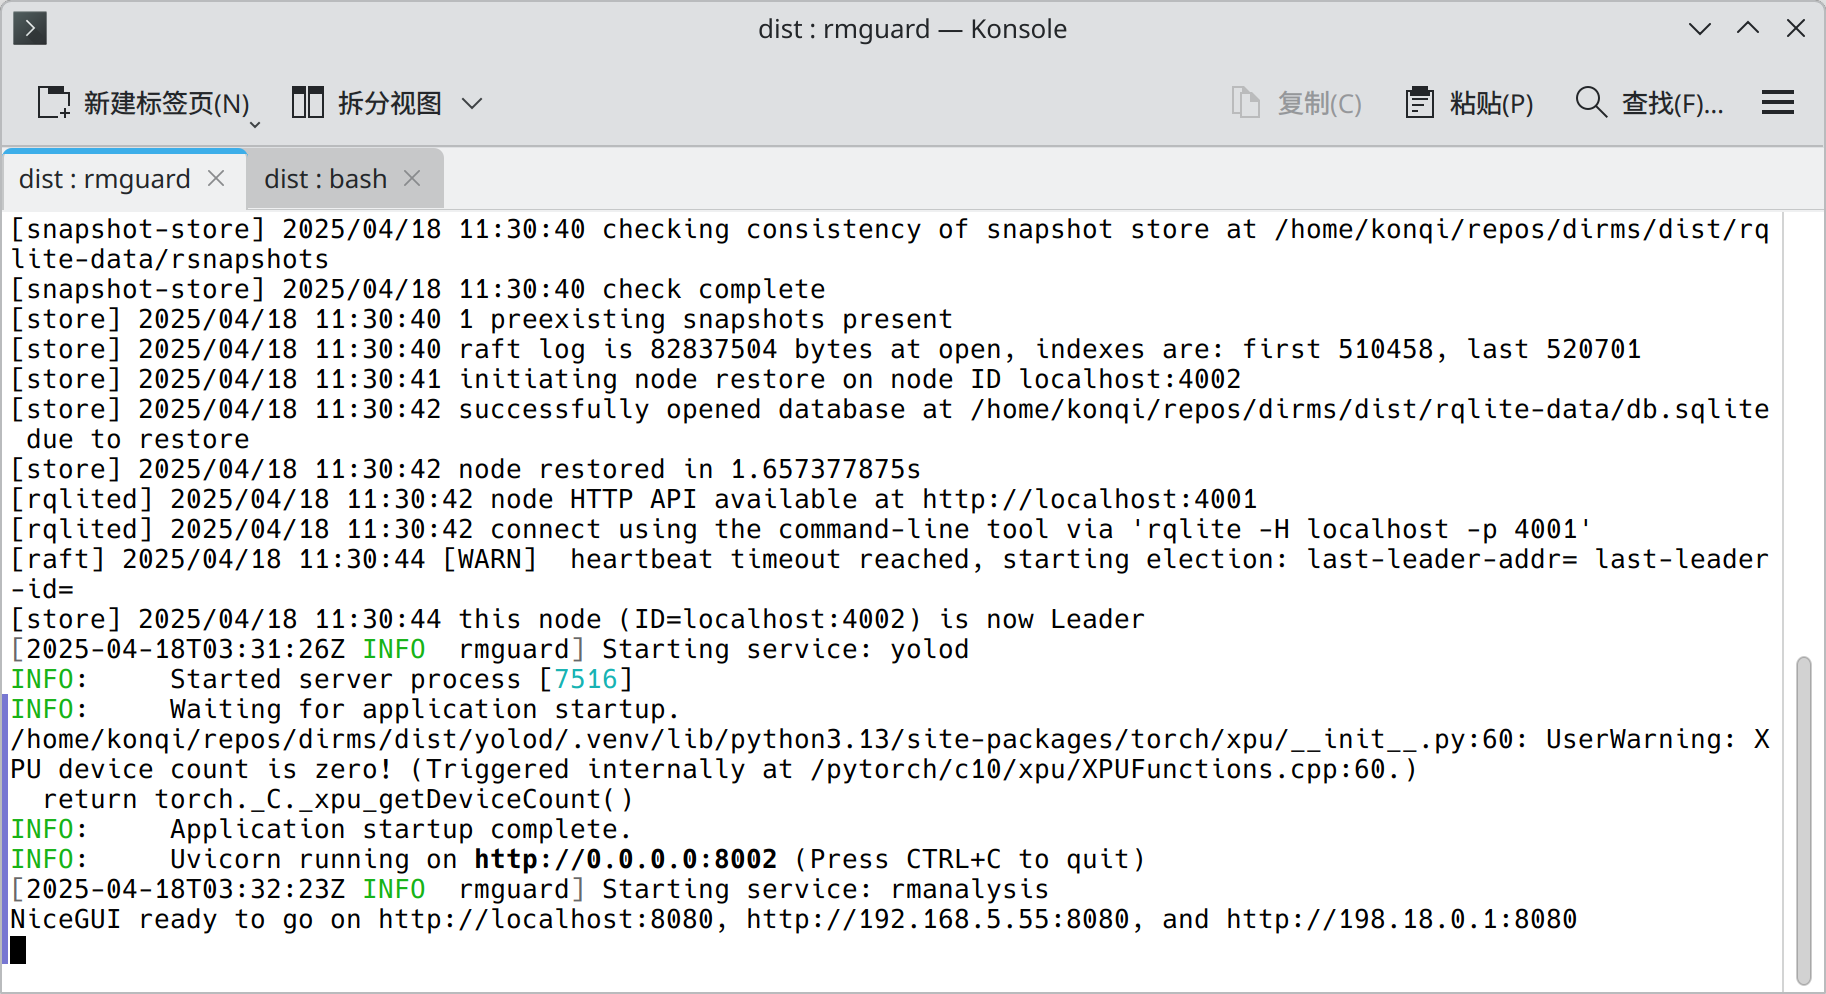
\includegraphics[width=0.45\textwidth]{./exp/rmg-rma-2.png}}
	\caption{(todo)}
	\label{fig:rmg-service}
\end{figure}

\subsection{商家端}

\subsubsection{RmAdmin}

\begin{figure}[htbp]
	\centering
	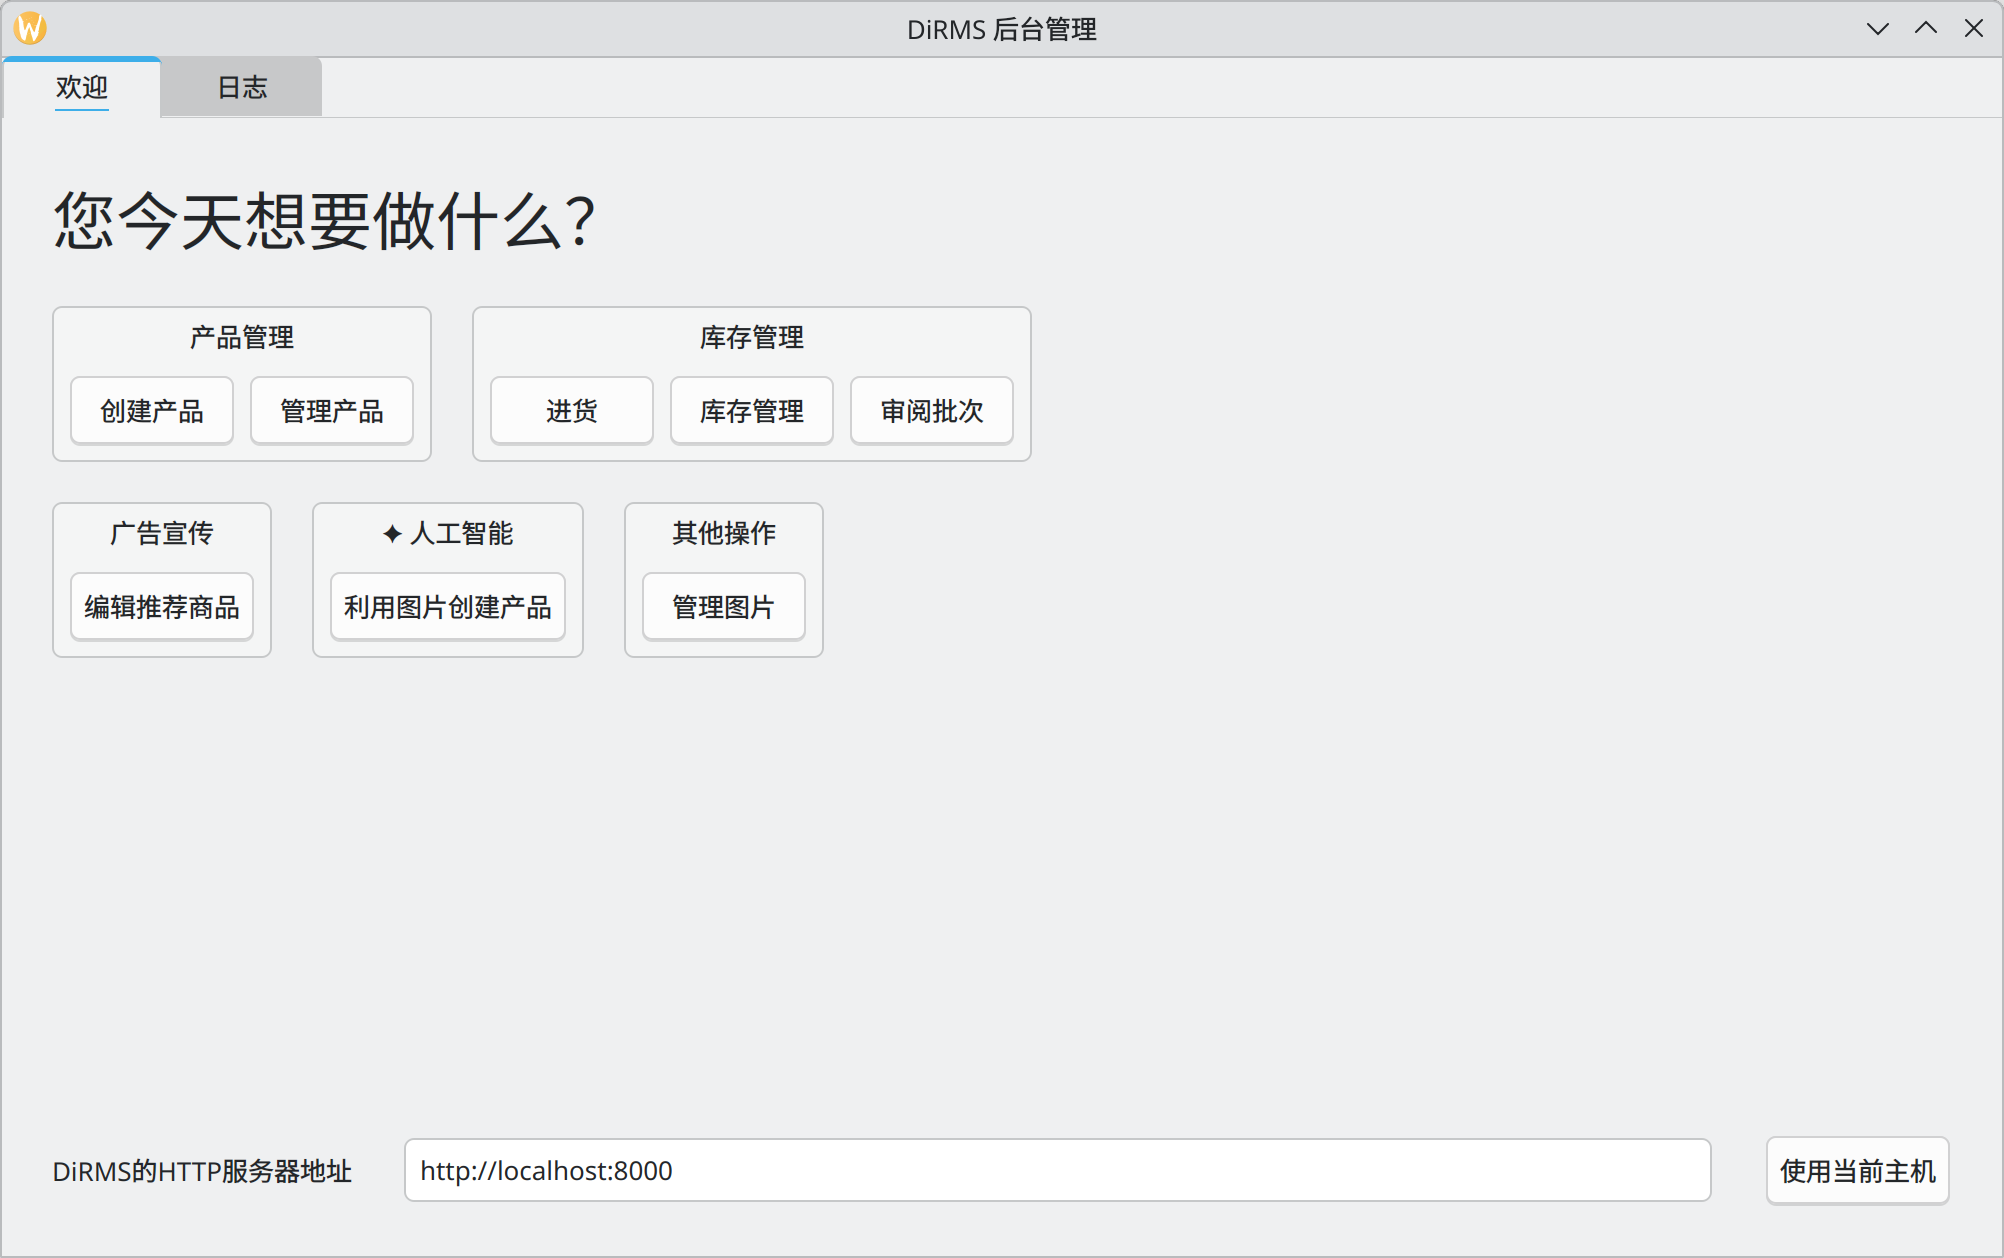
\includegraphics[width=0.8\textwidth]{./exp/rma-index.png}
	\caption{(todo)}
	\label{fig:rma-index}
\end{figure}

\begin{figure}[htbp]
    \subfloat{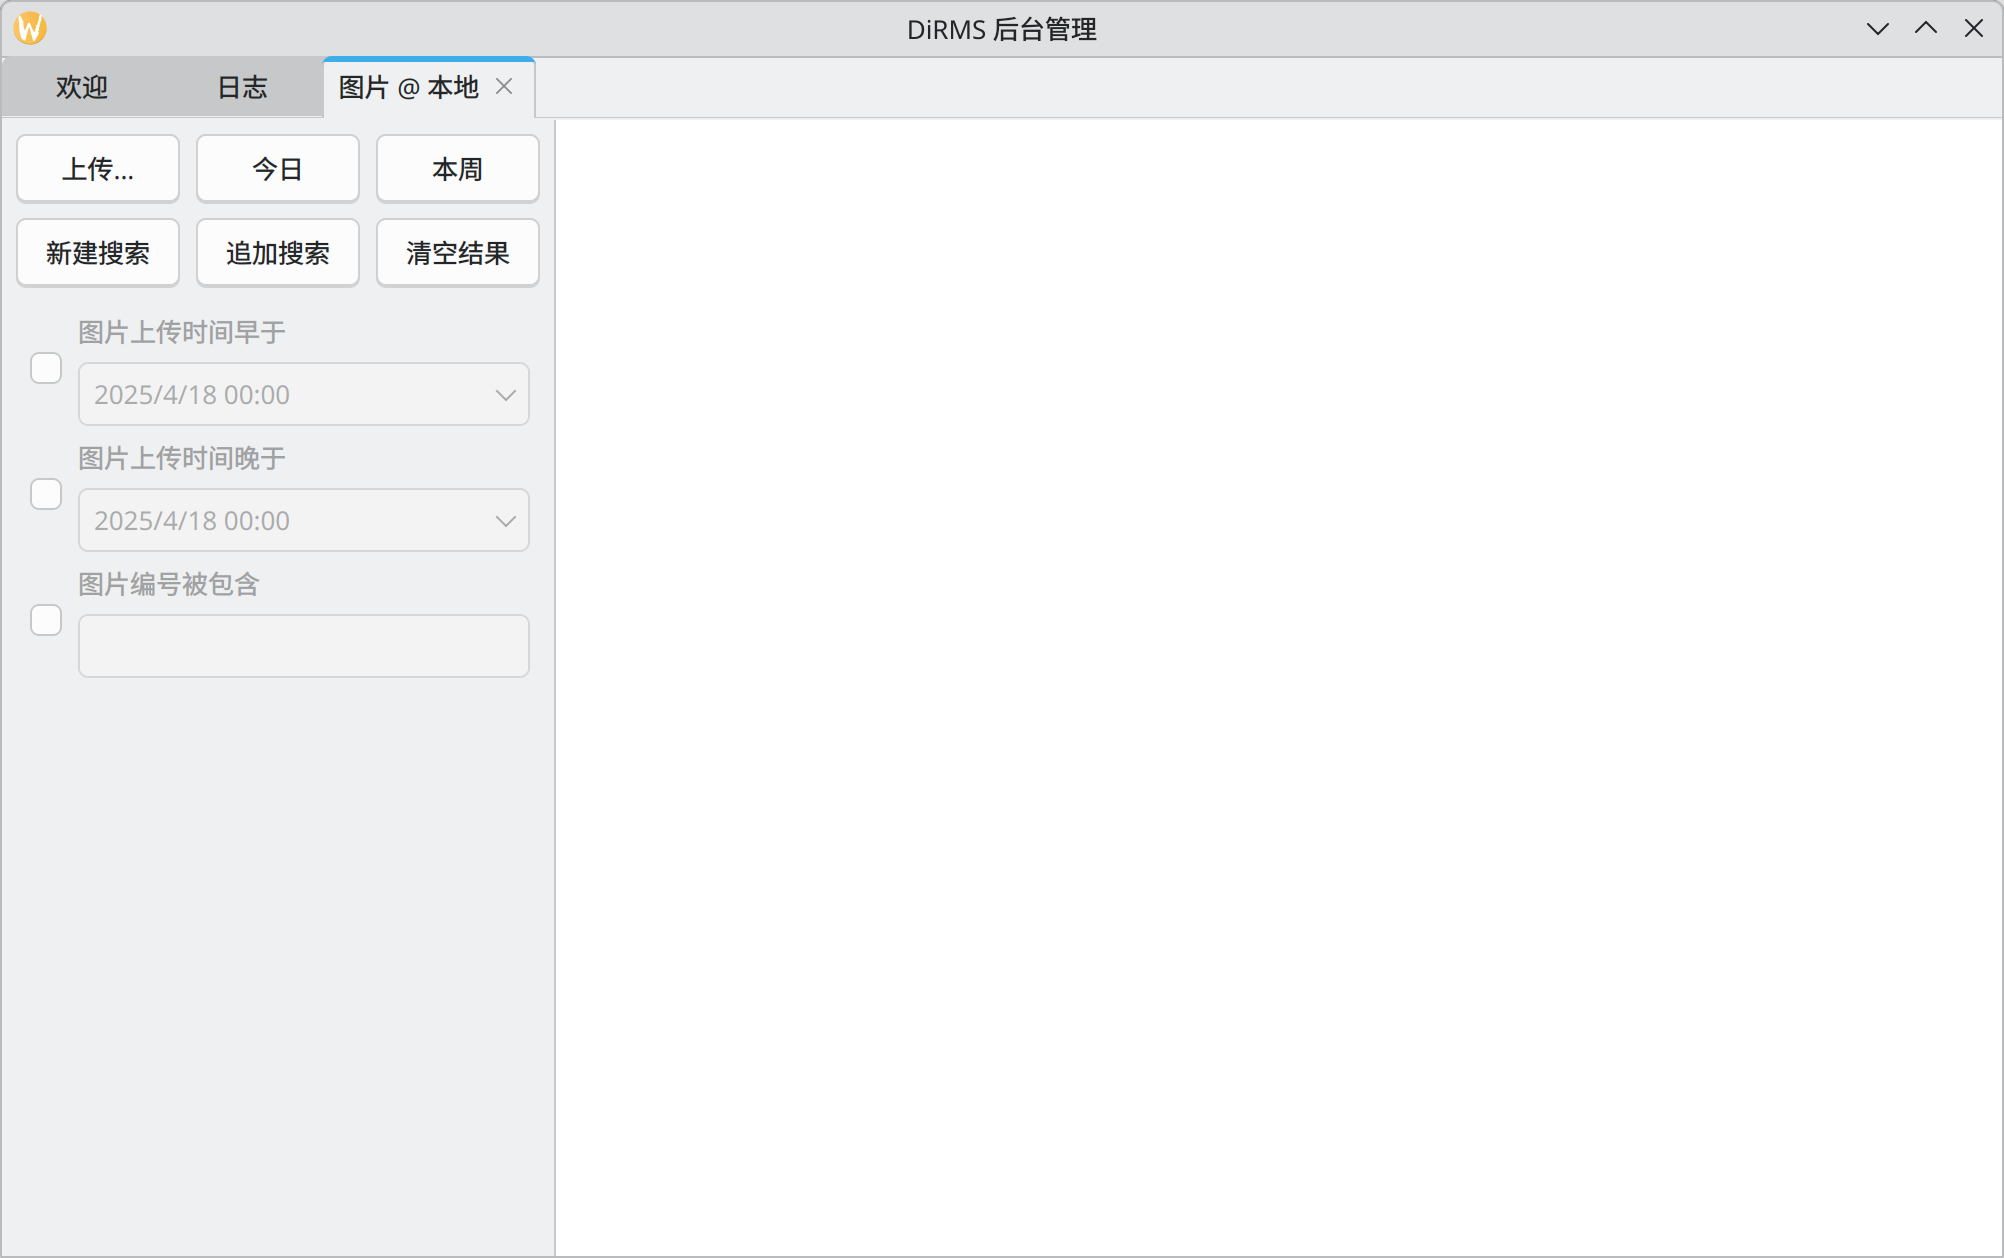
\includegraphics[width=0.45\textwidth]{./exp/rma-im-add-1.png}}
    \hfill
    \subfloat{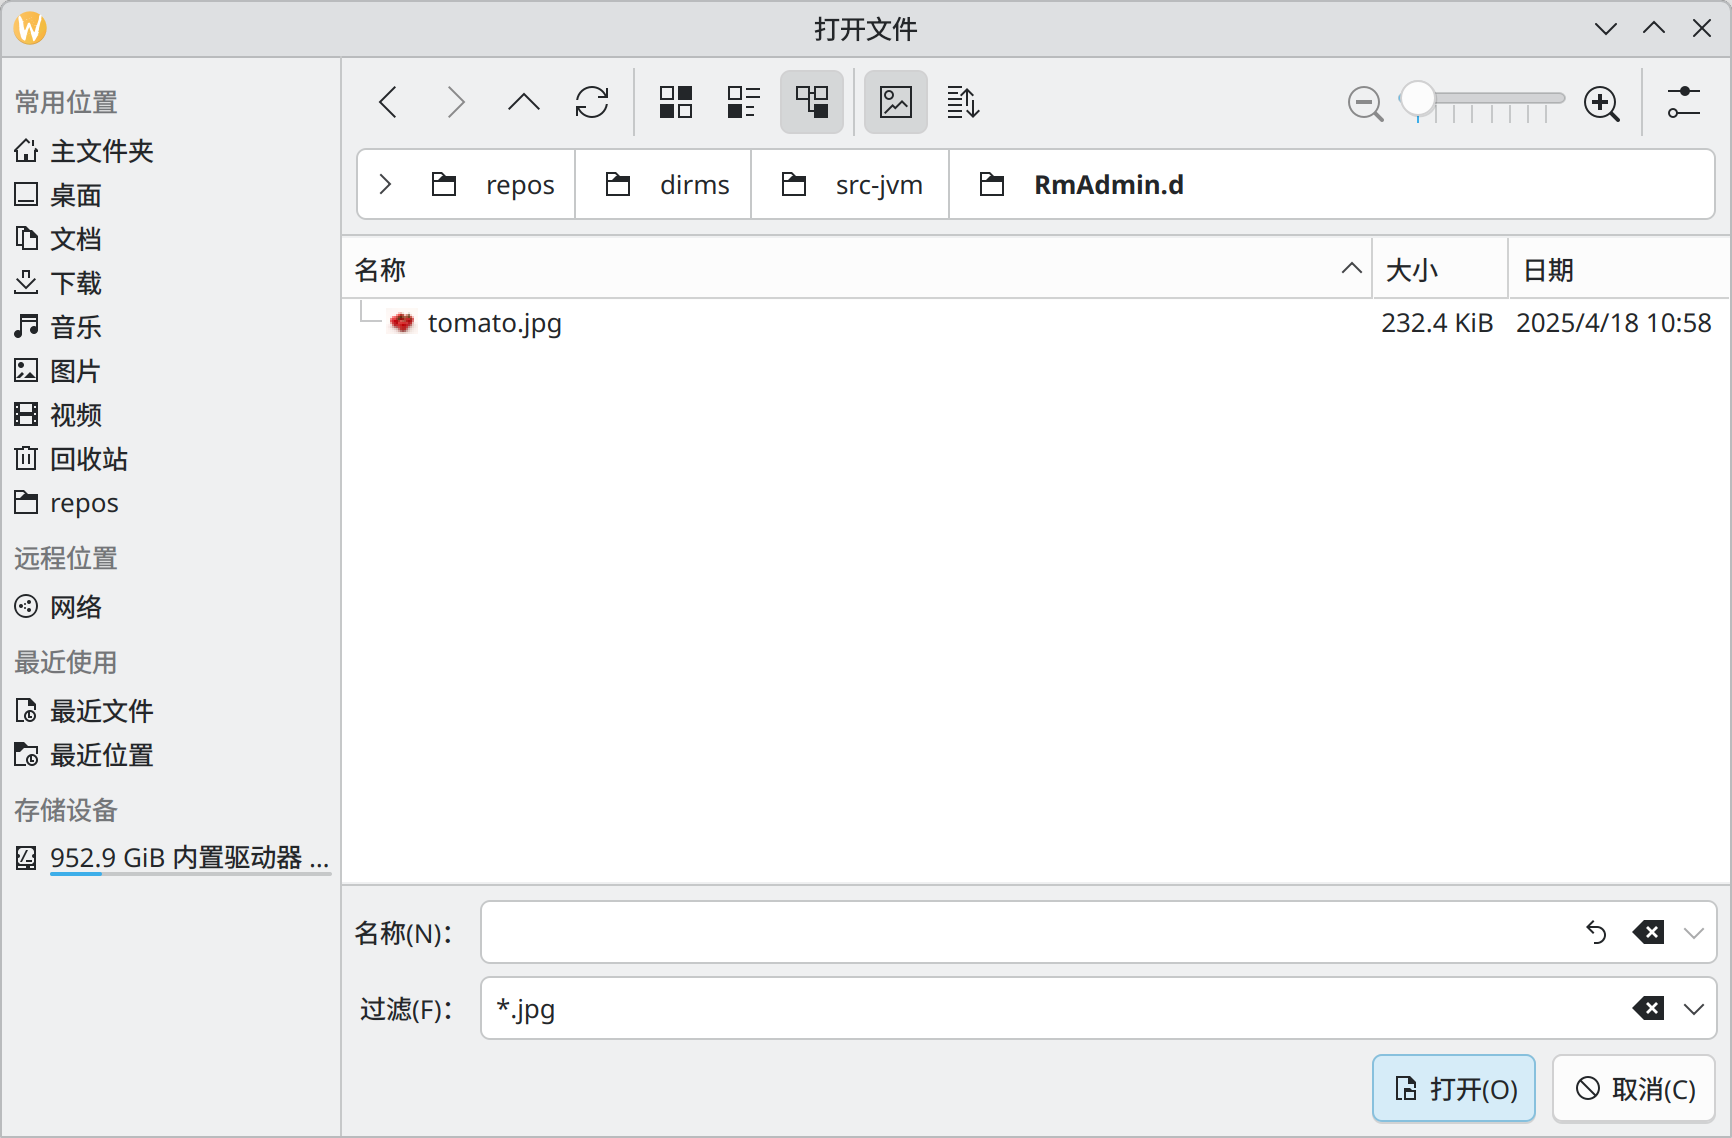
\includegraphics[width=0.45\textwidth]{./exp/rma-im-add-2.png}}
	\caption{(todo)}
	\label{fig:rma-im-add}
\end{figure}

\begin{figure}[htbp]
	\centering
	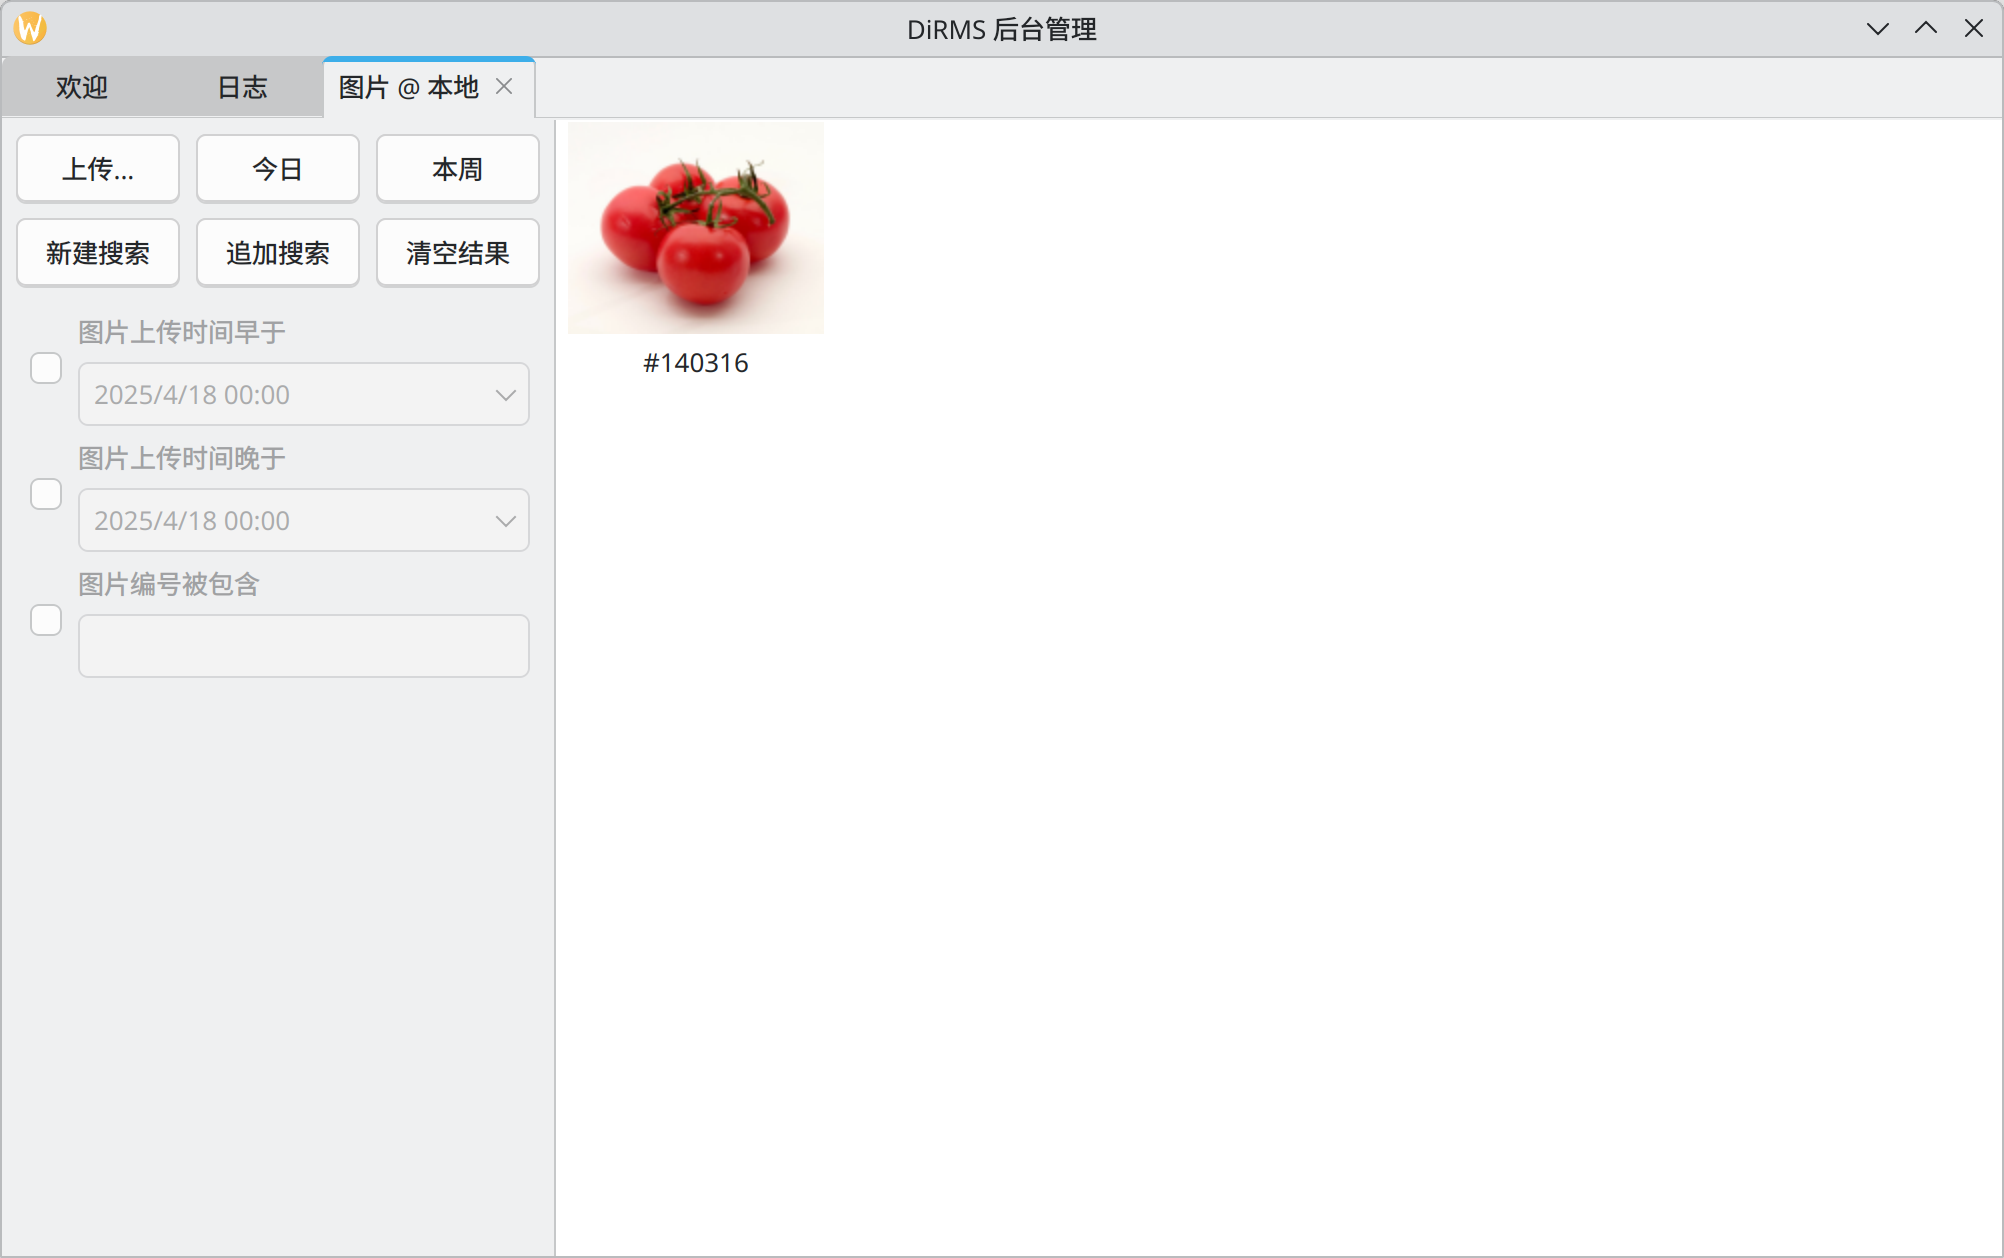
\includegraphics[width=0.8\textwidth]{./exp/rma-im-as.png}
	\caption{(todo)}
	\label{fig:rma-im-as}
\end{figure}

\begin{figure}[htbp]
    \subfloat{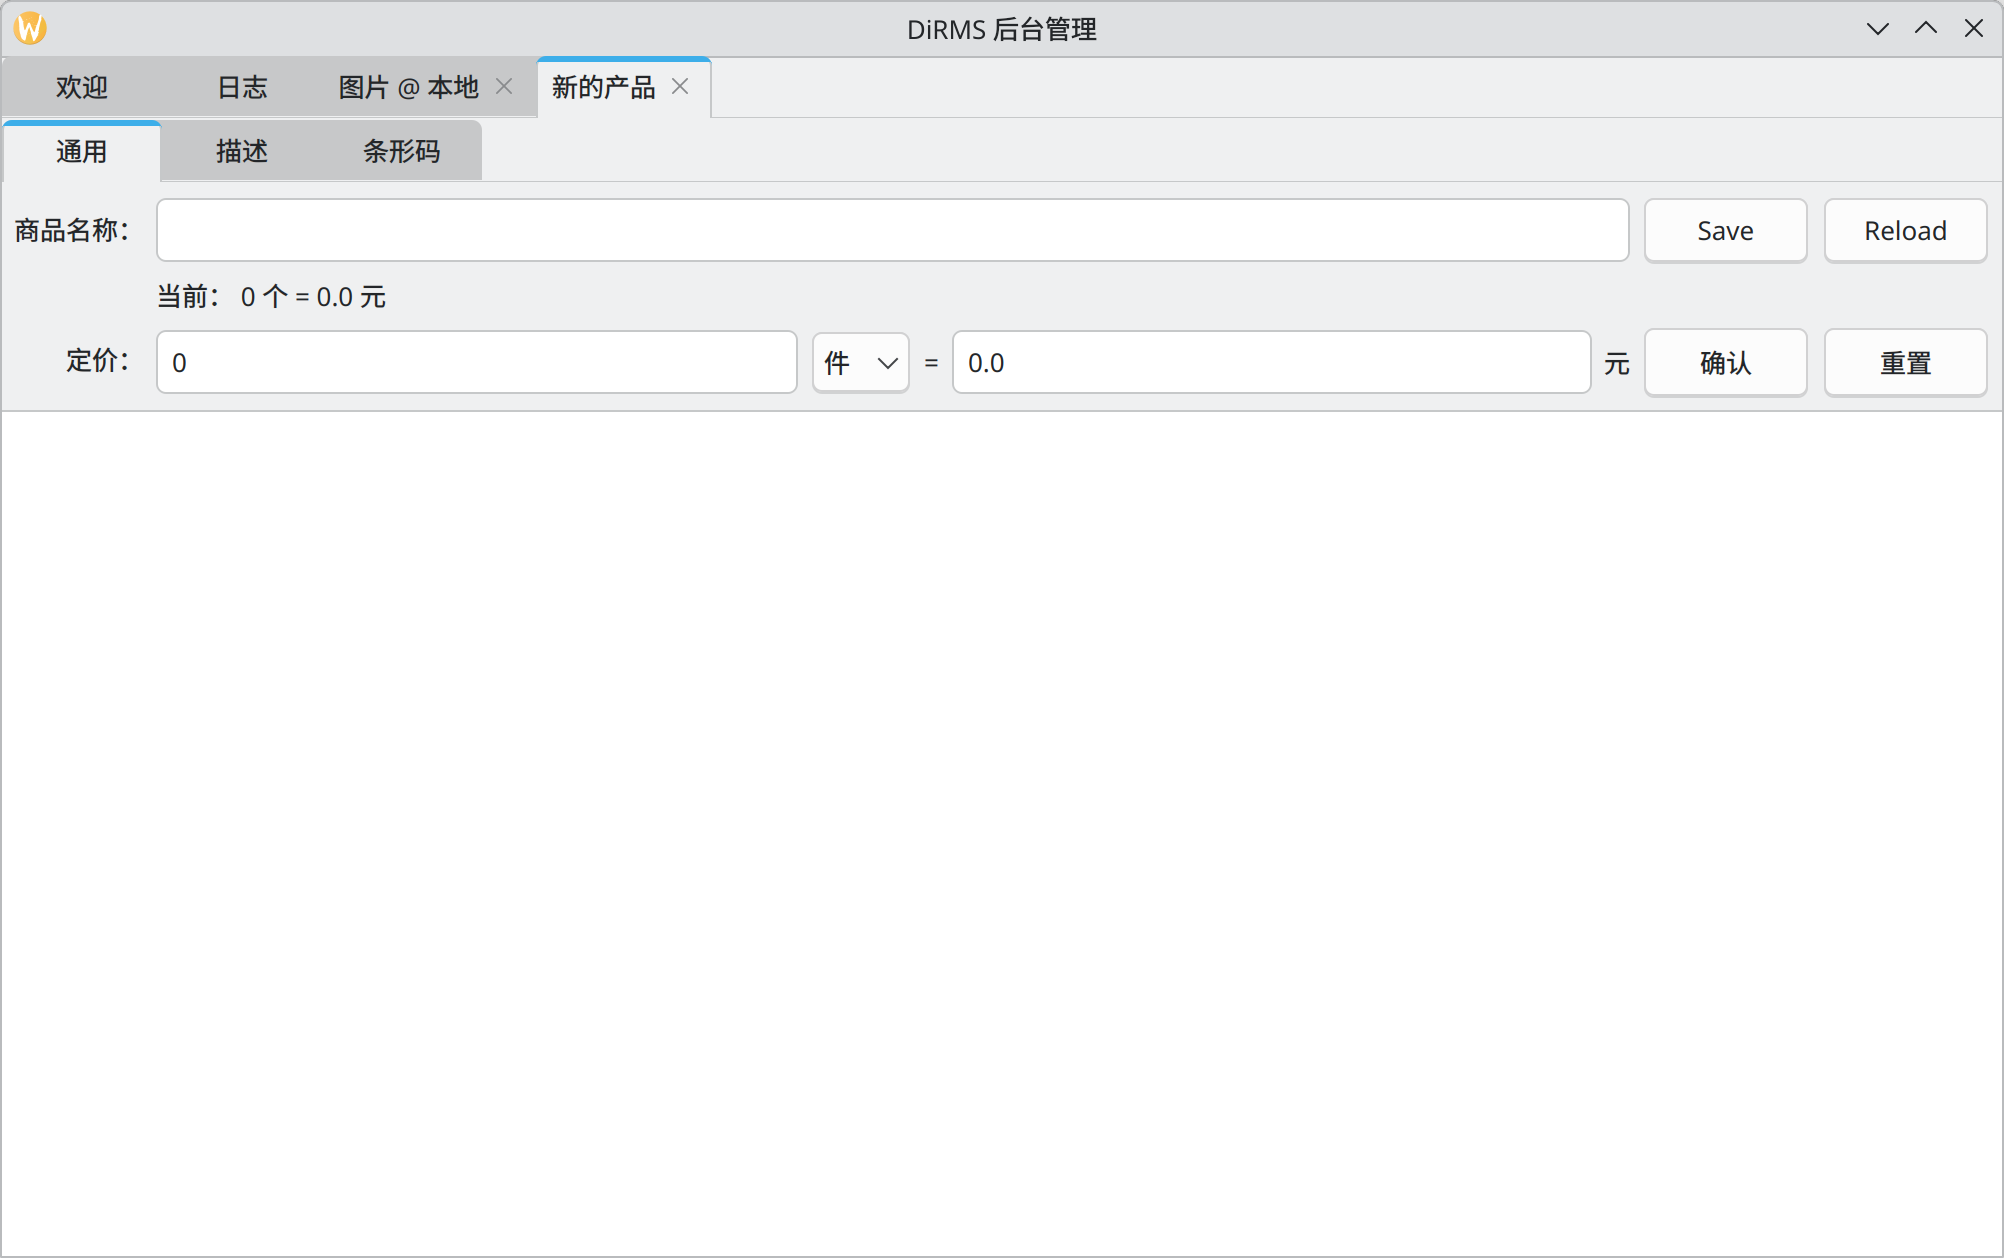
\includegraphics[width=0.3\textwidth]{./exp/rma-prod-add-1.png}}
    \hfill
    \subfloat{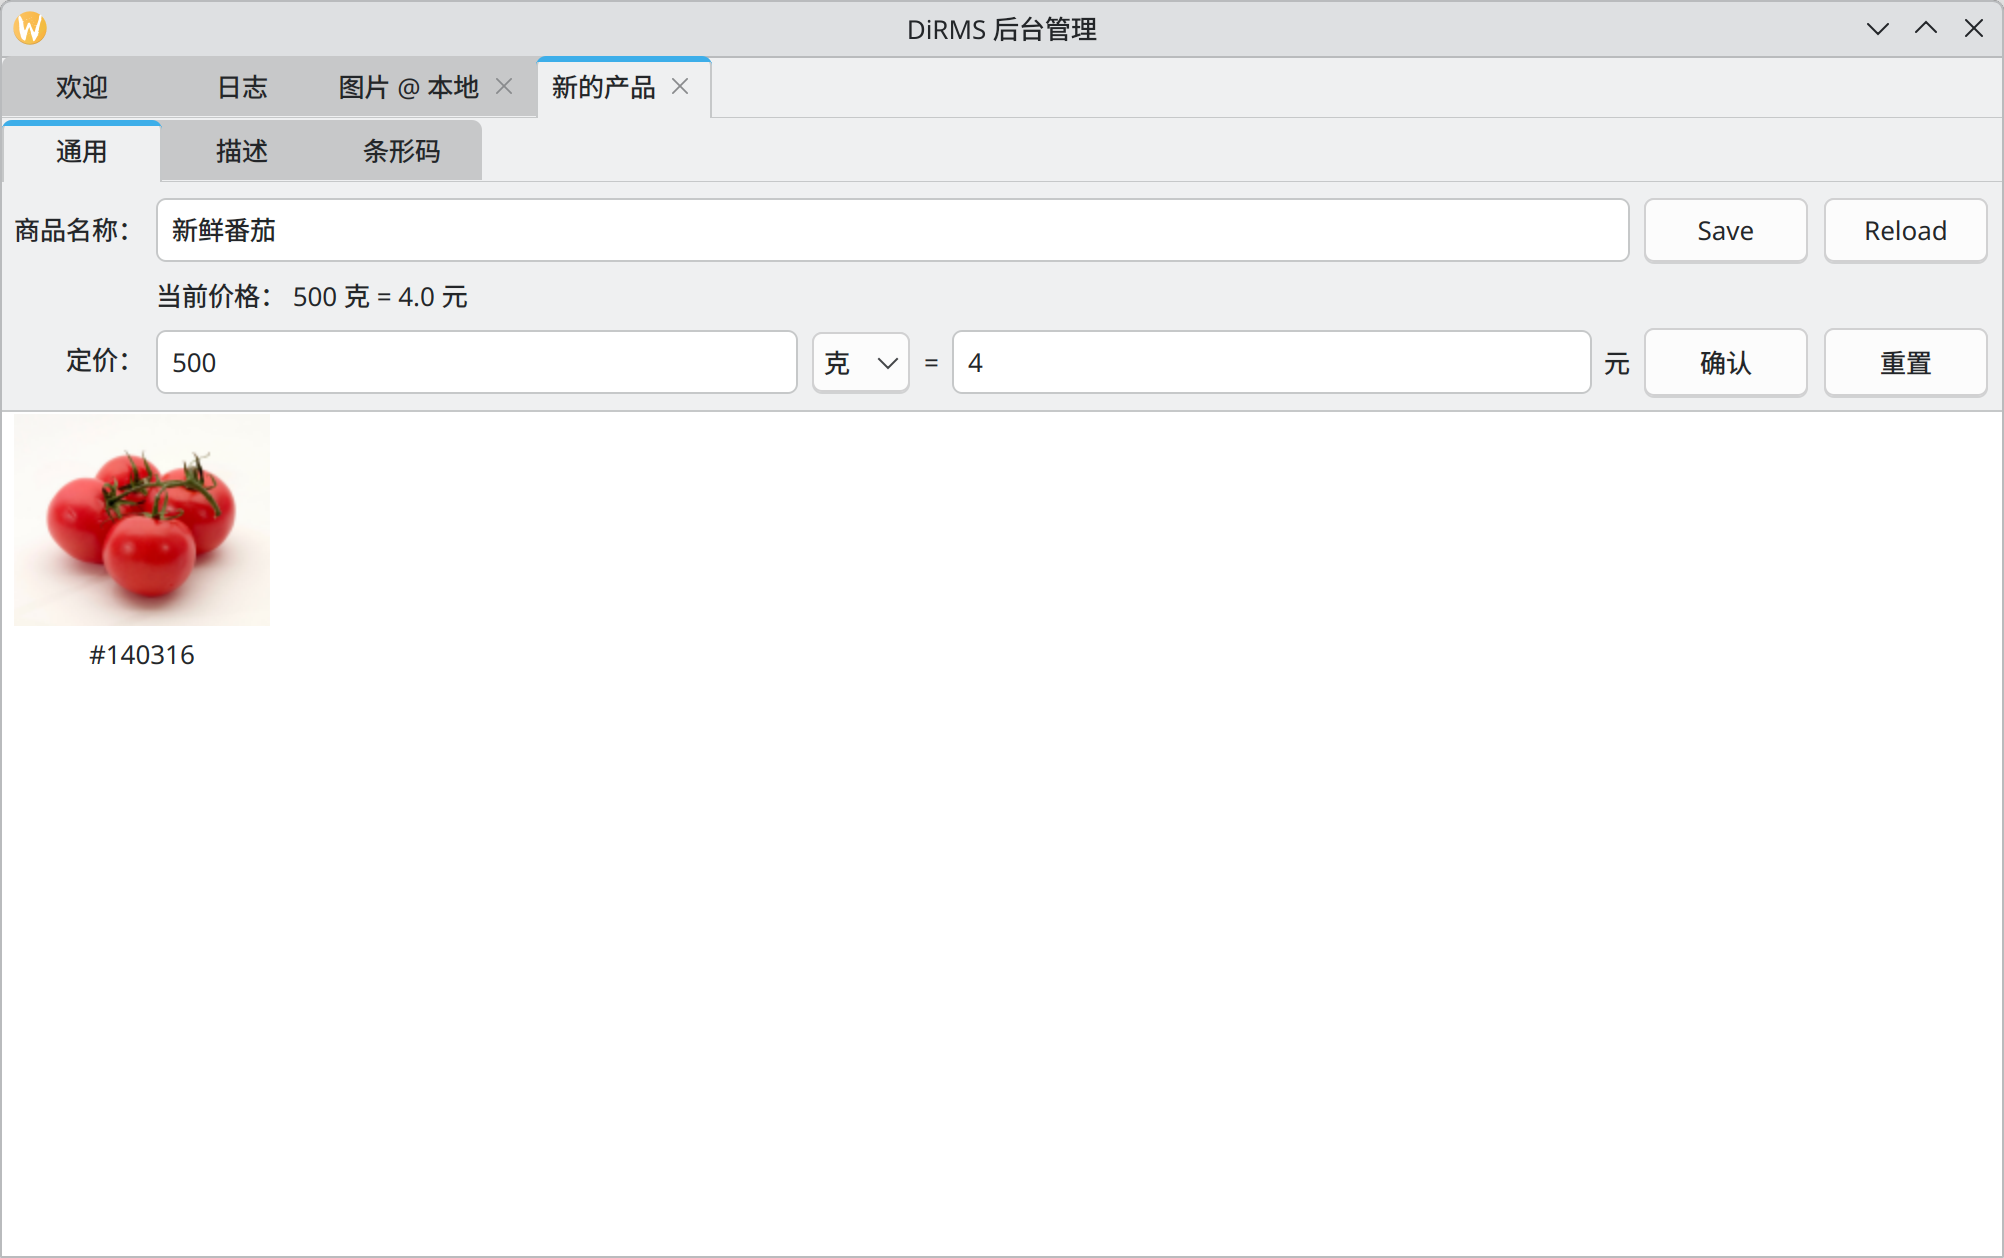
\includegraphics[width=0.3\textwidth]{./exp/rma-prod-add-2.png}}
    \hfill
    \subfloat{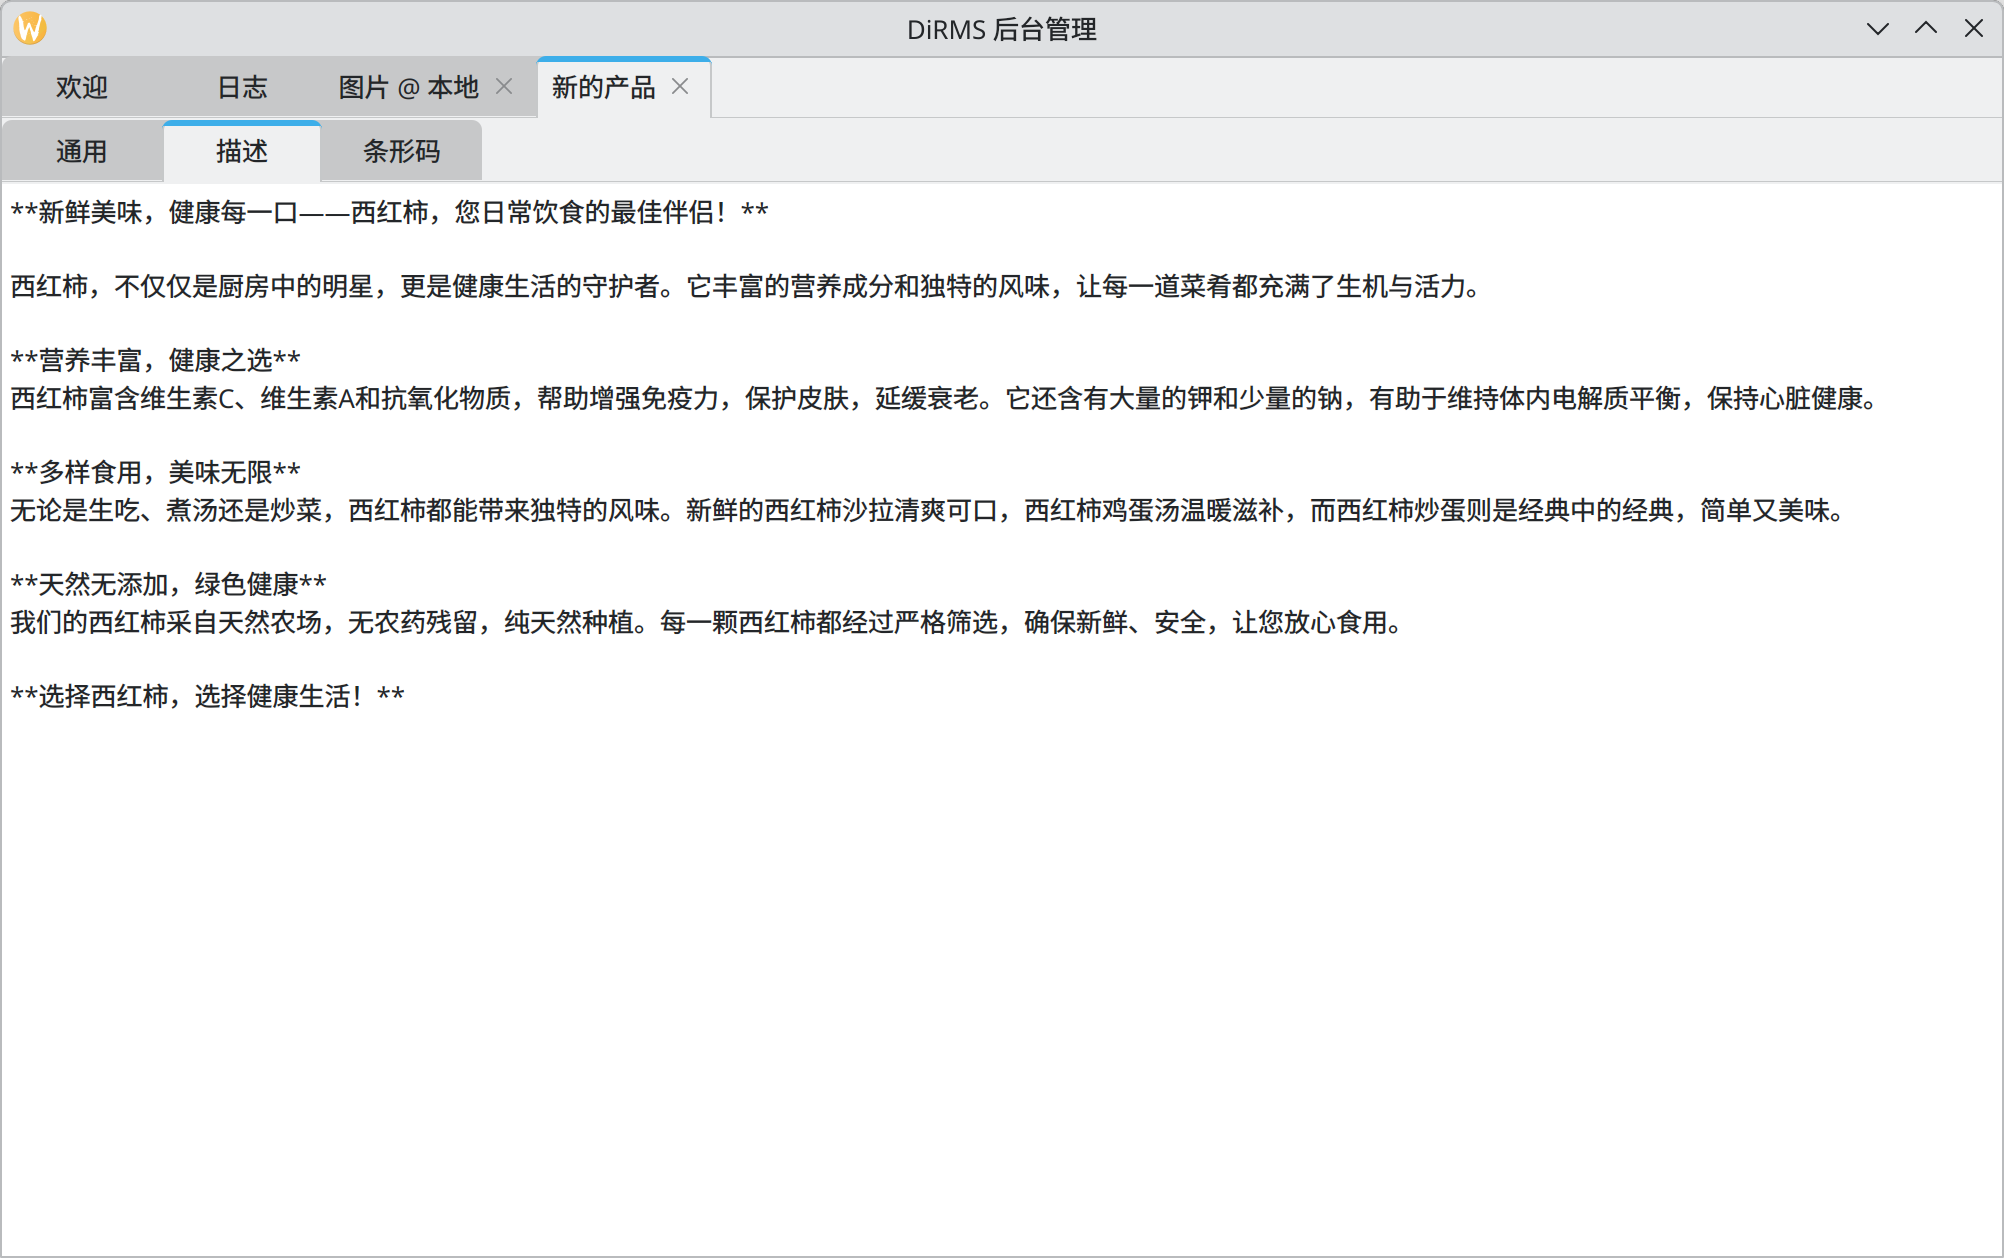
\includegraphics[width=0.3\textwidth]{./exp/rma-prod-add-3.png}}
	\caption{(todo)}
	\label{fig:rma-prod-add}
\end{figure}

\begin{figure}[htbp]
    \subfloat{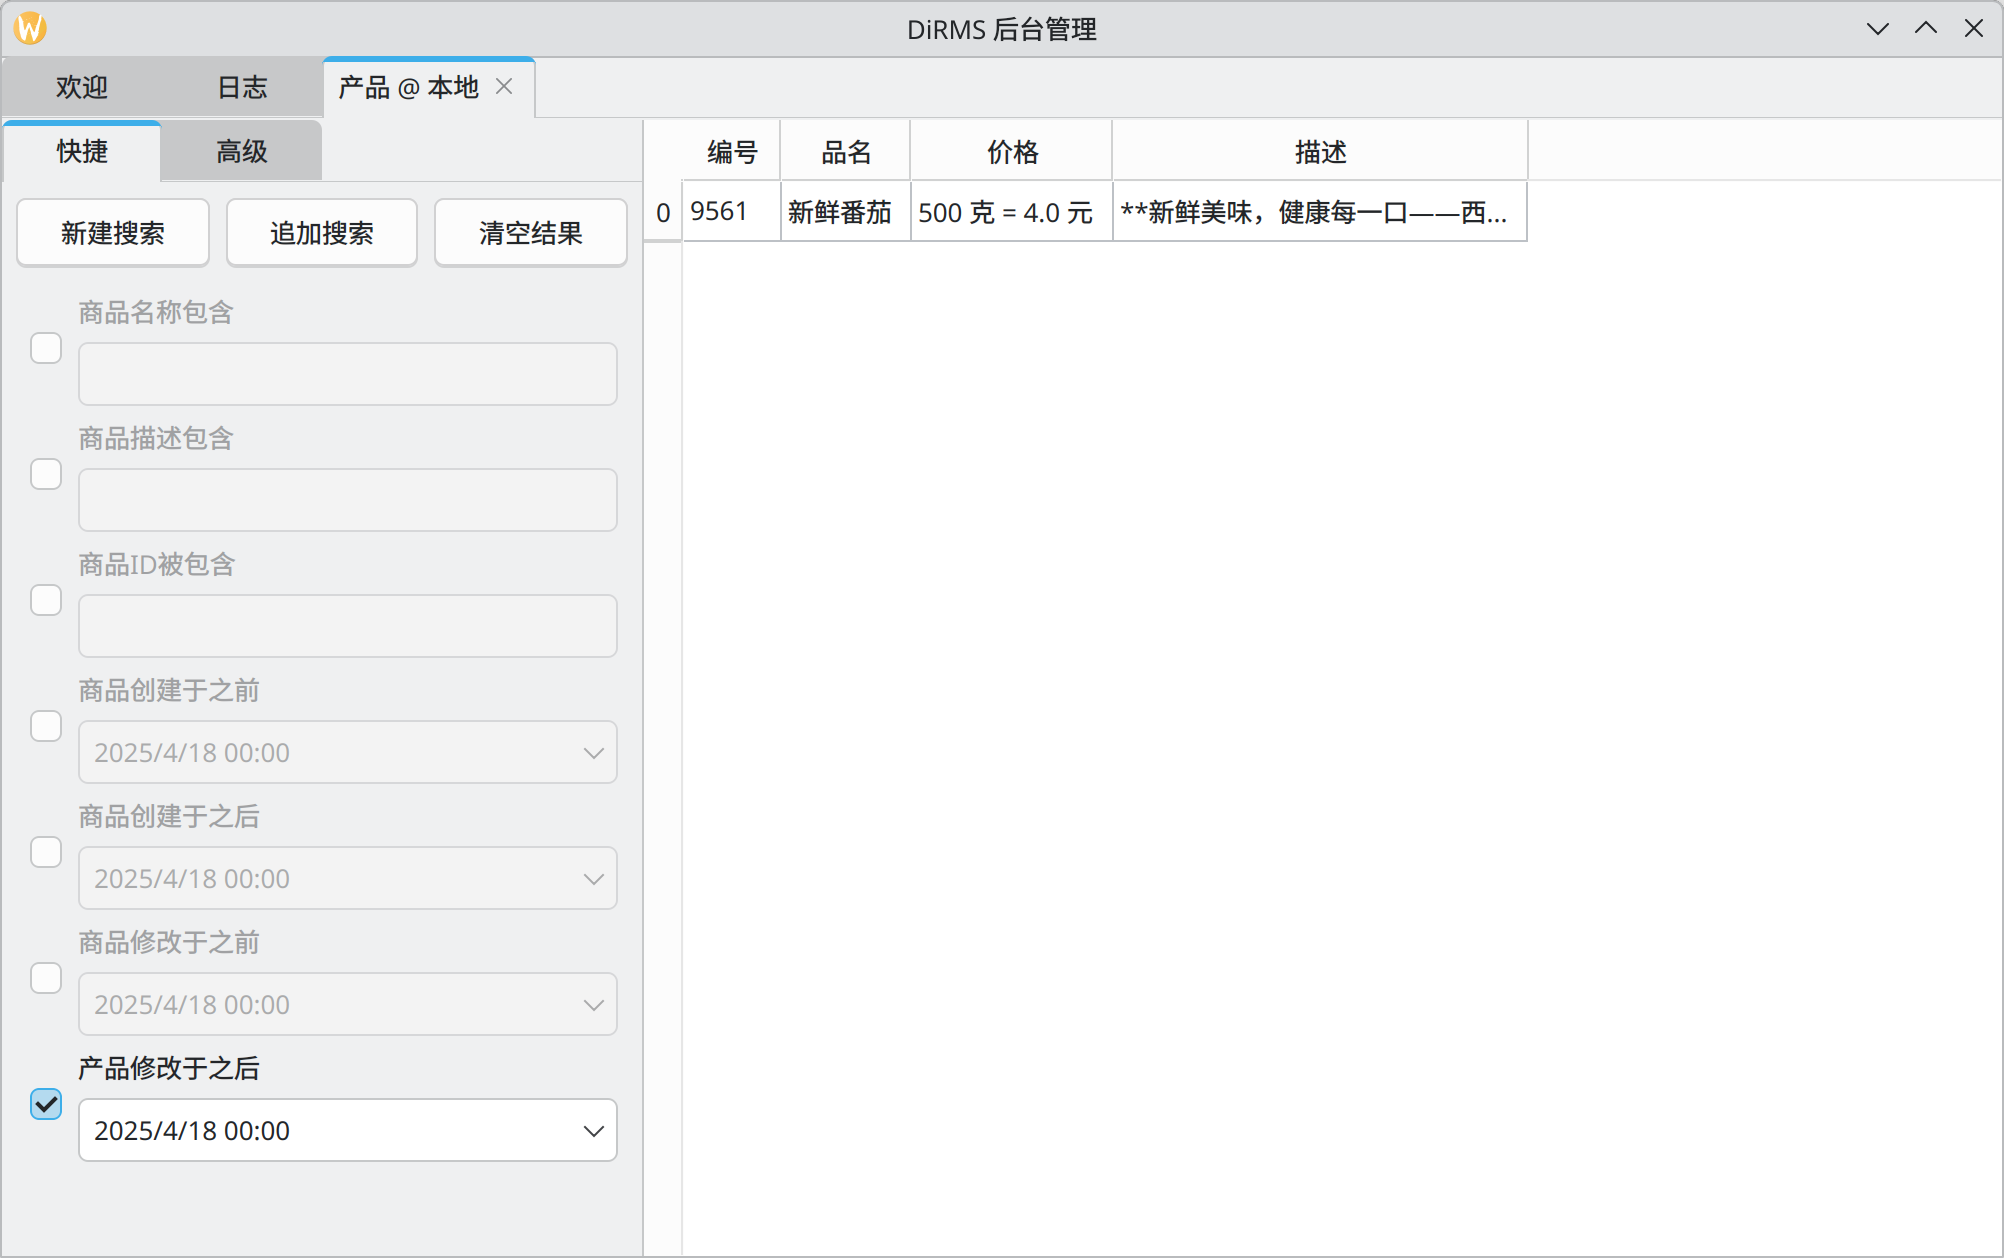
\includegraphics[width=0.3\textwidth]{./exp/rma-prod-as-1.png}}
    \hfill
    \subfloat{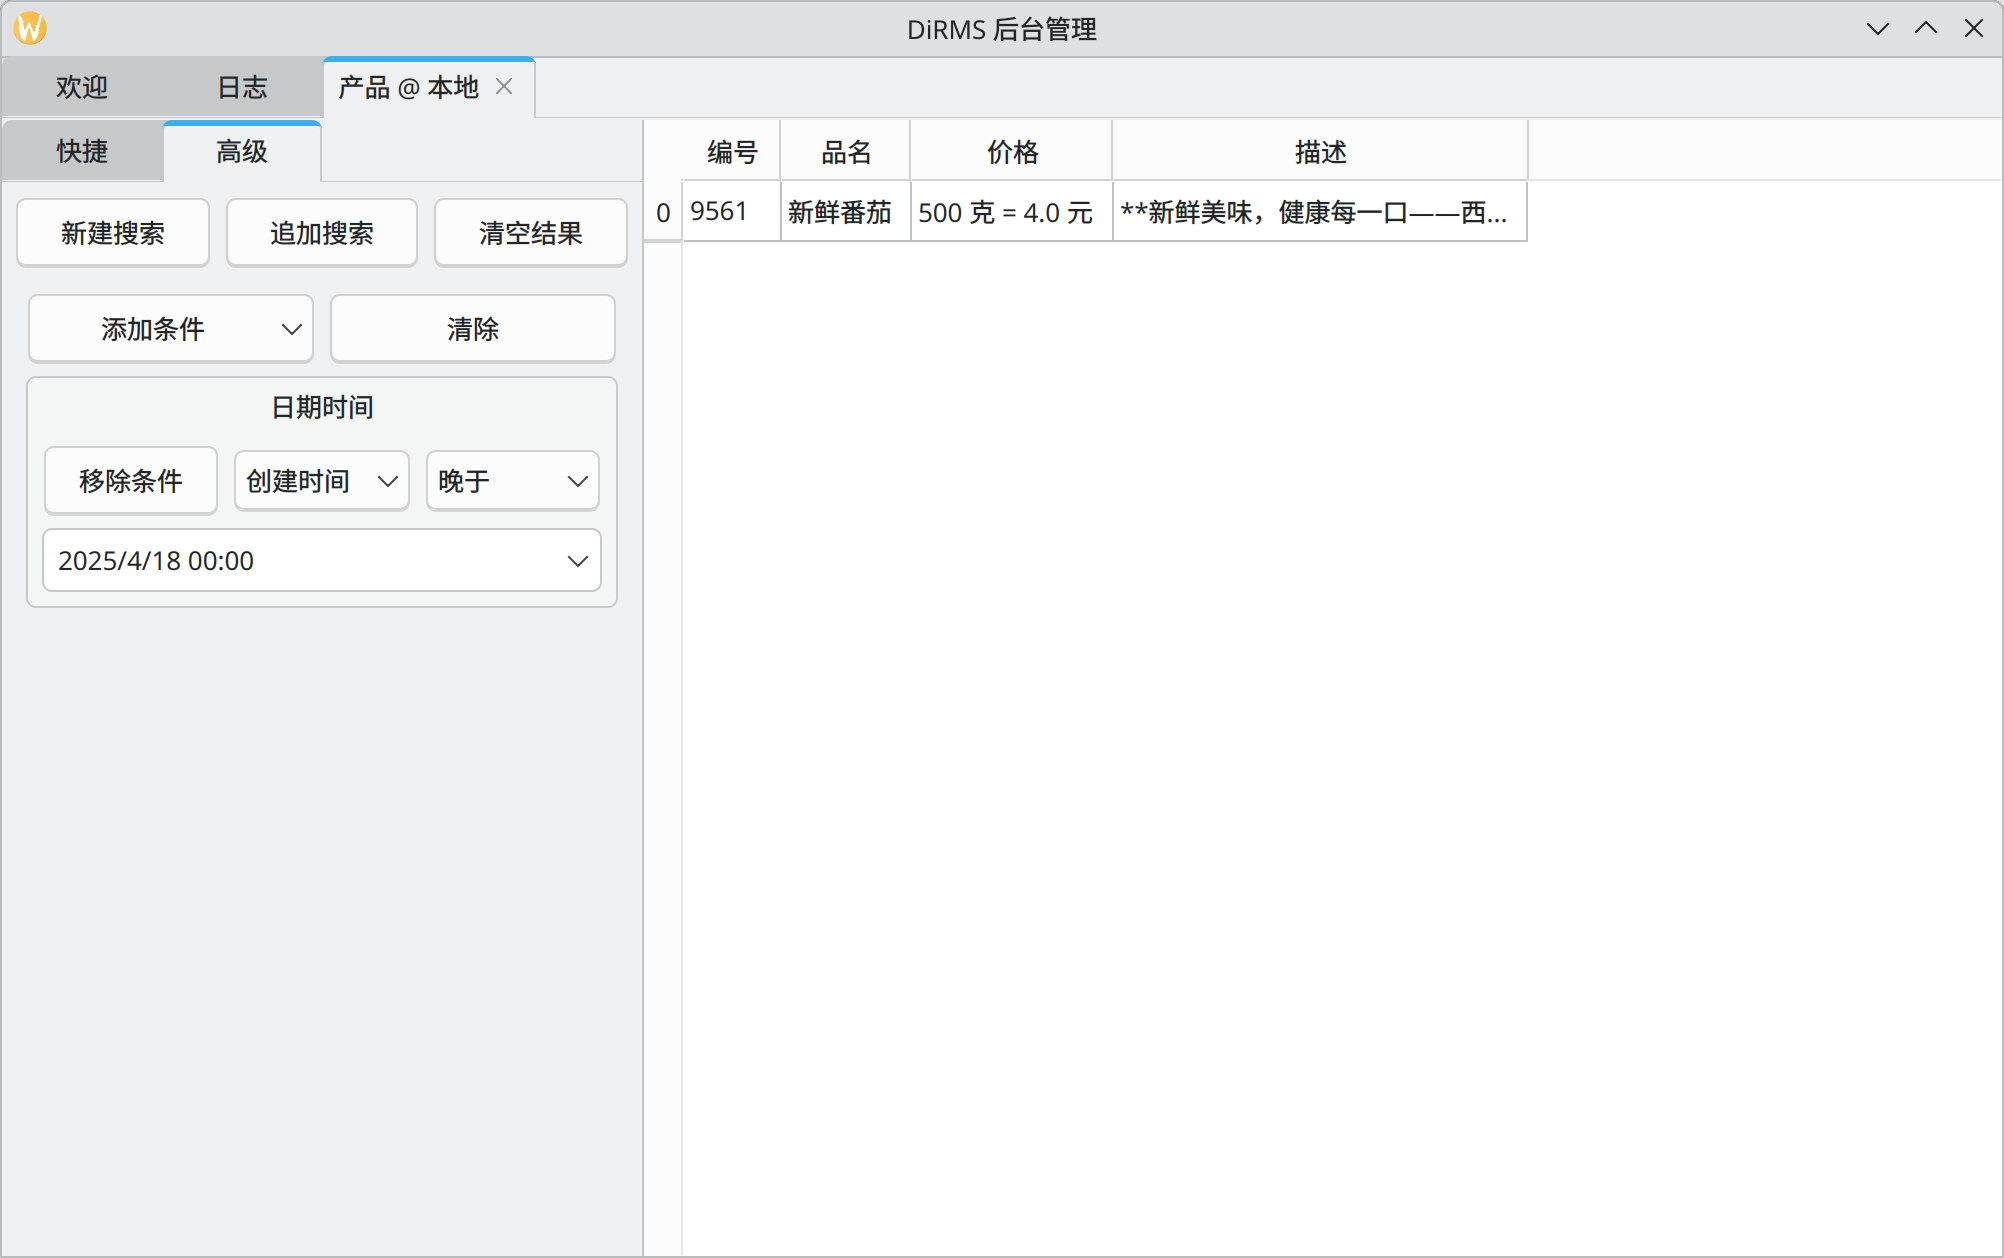
\includegraphics[width=0.3\textwidth]{./exp/rma-prod-as-2.png}}
    \hfill
    \subfloat{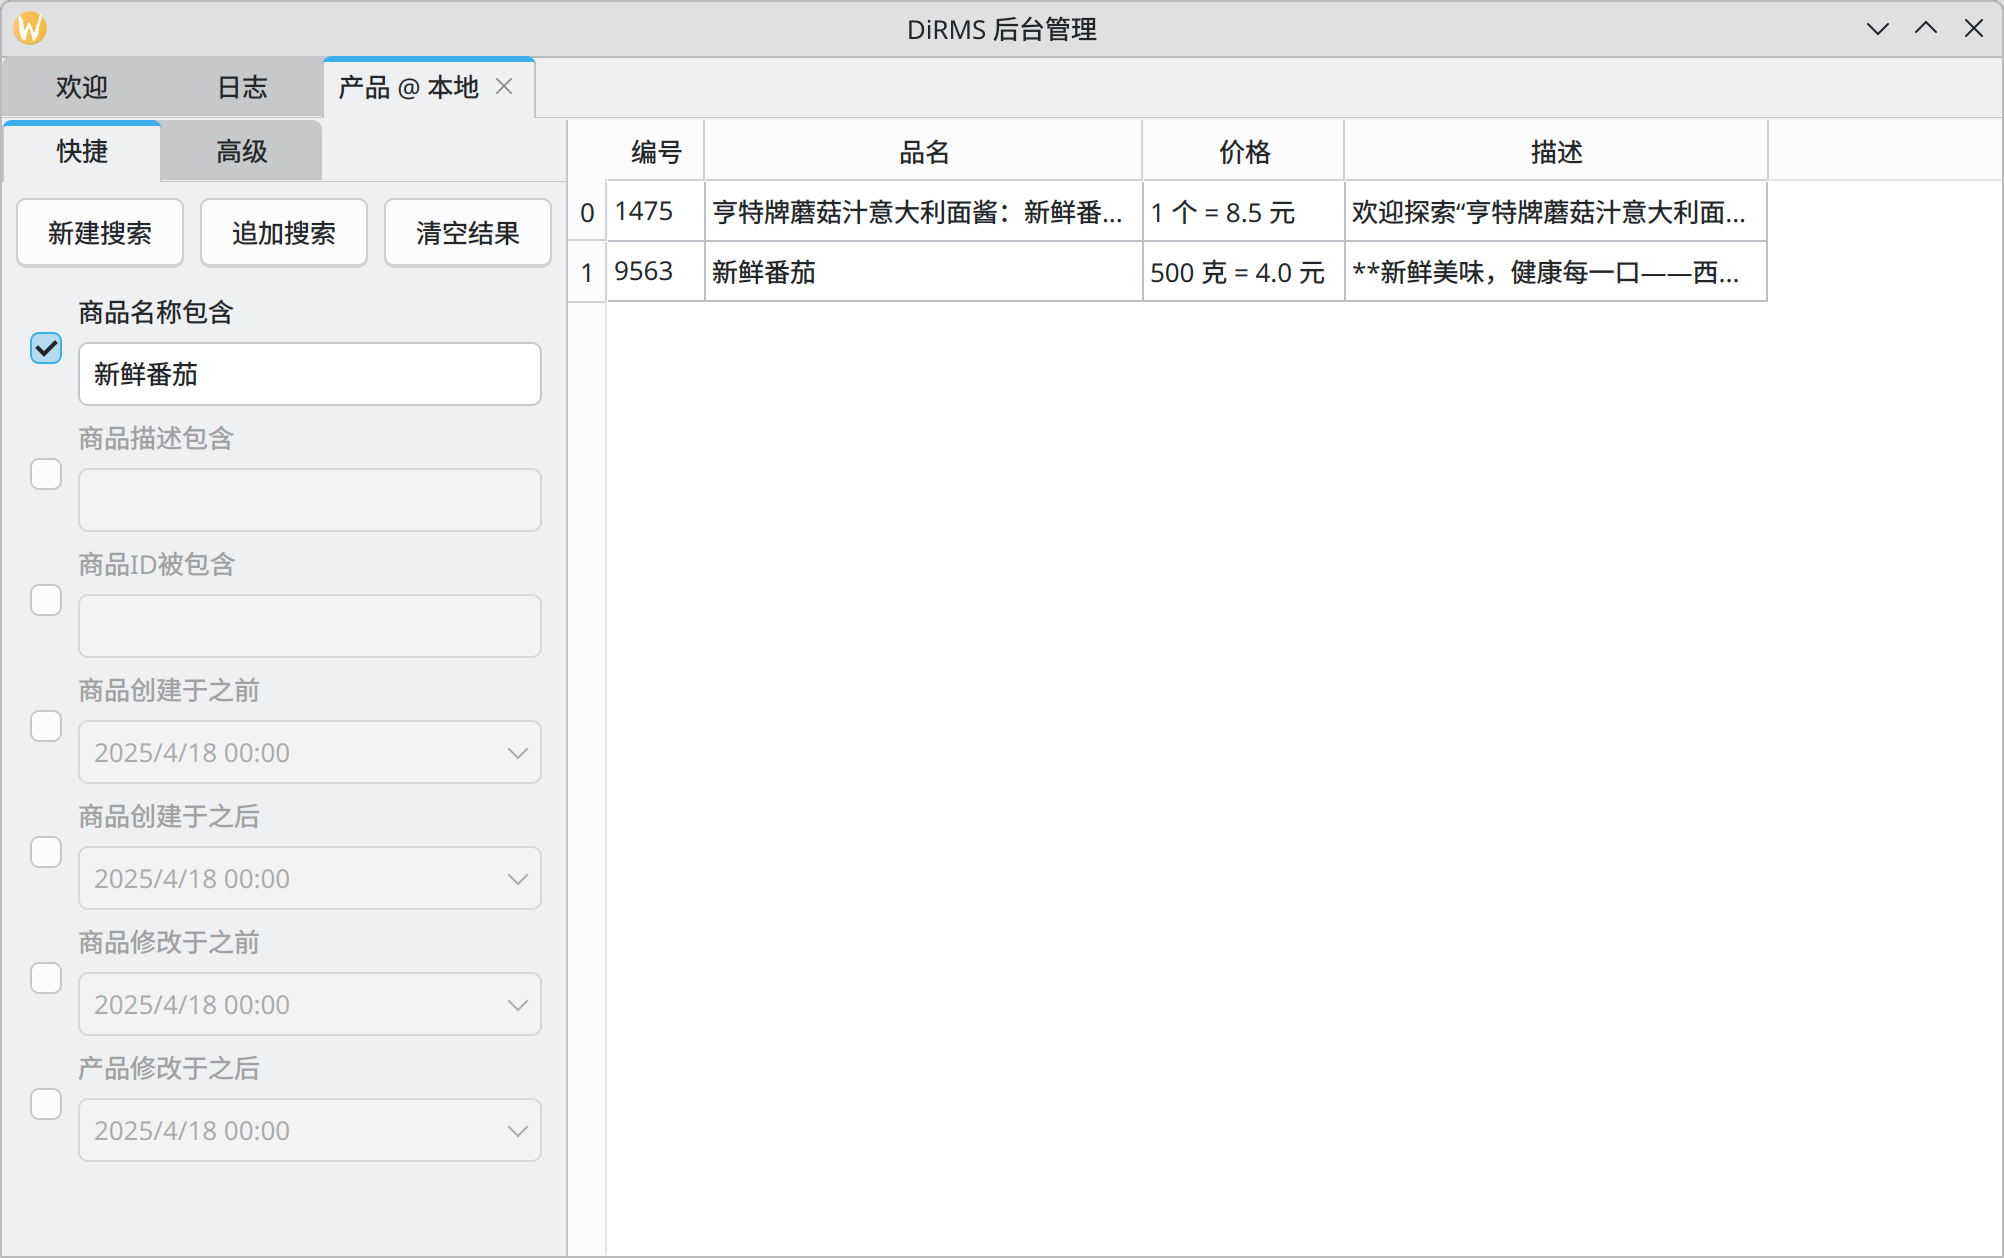
\includegraphics[width=0.3\textwidth]{./exp/rma-prod-as-3.png}}
	\caption{(todo)}
	\label{fig:rma-prod-as}
\end{figure}

\begin{figure}[htbp]
    \subfloat{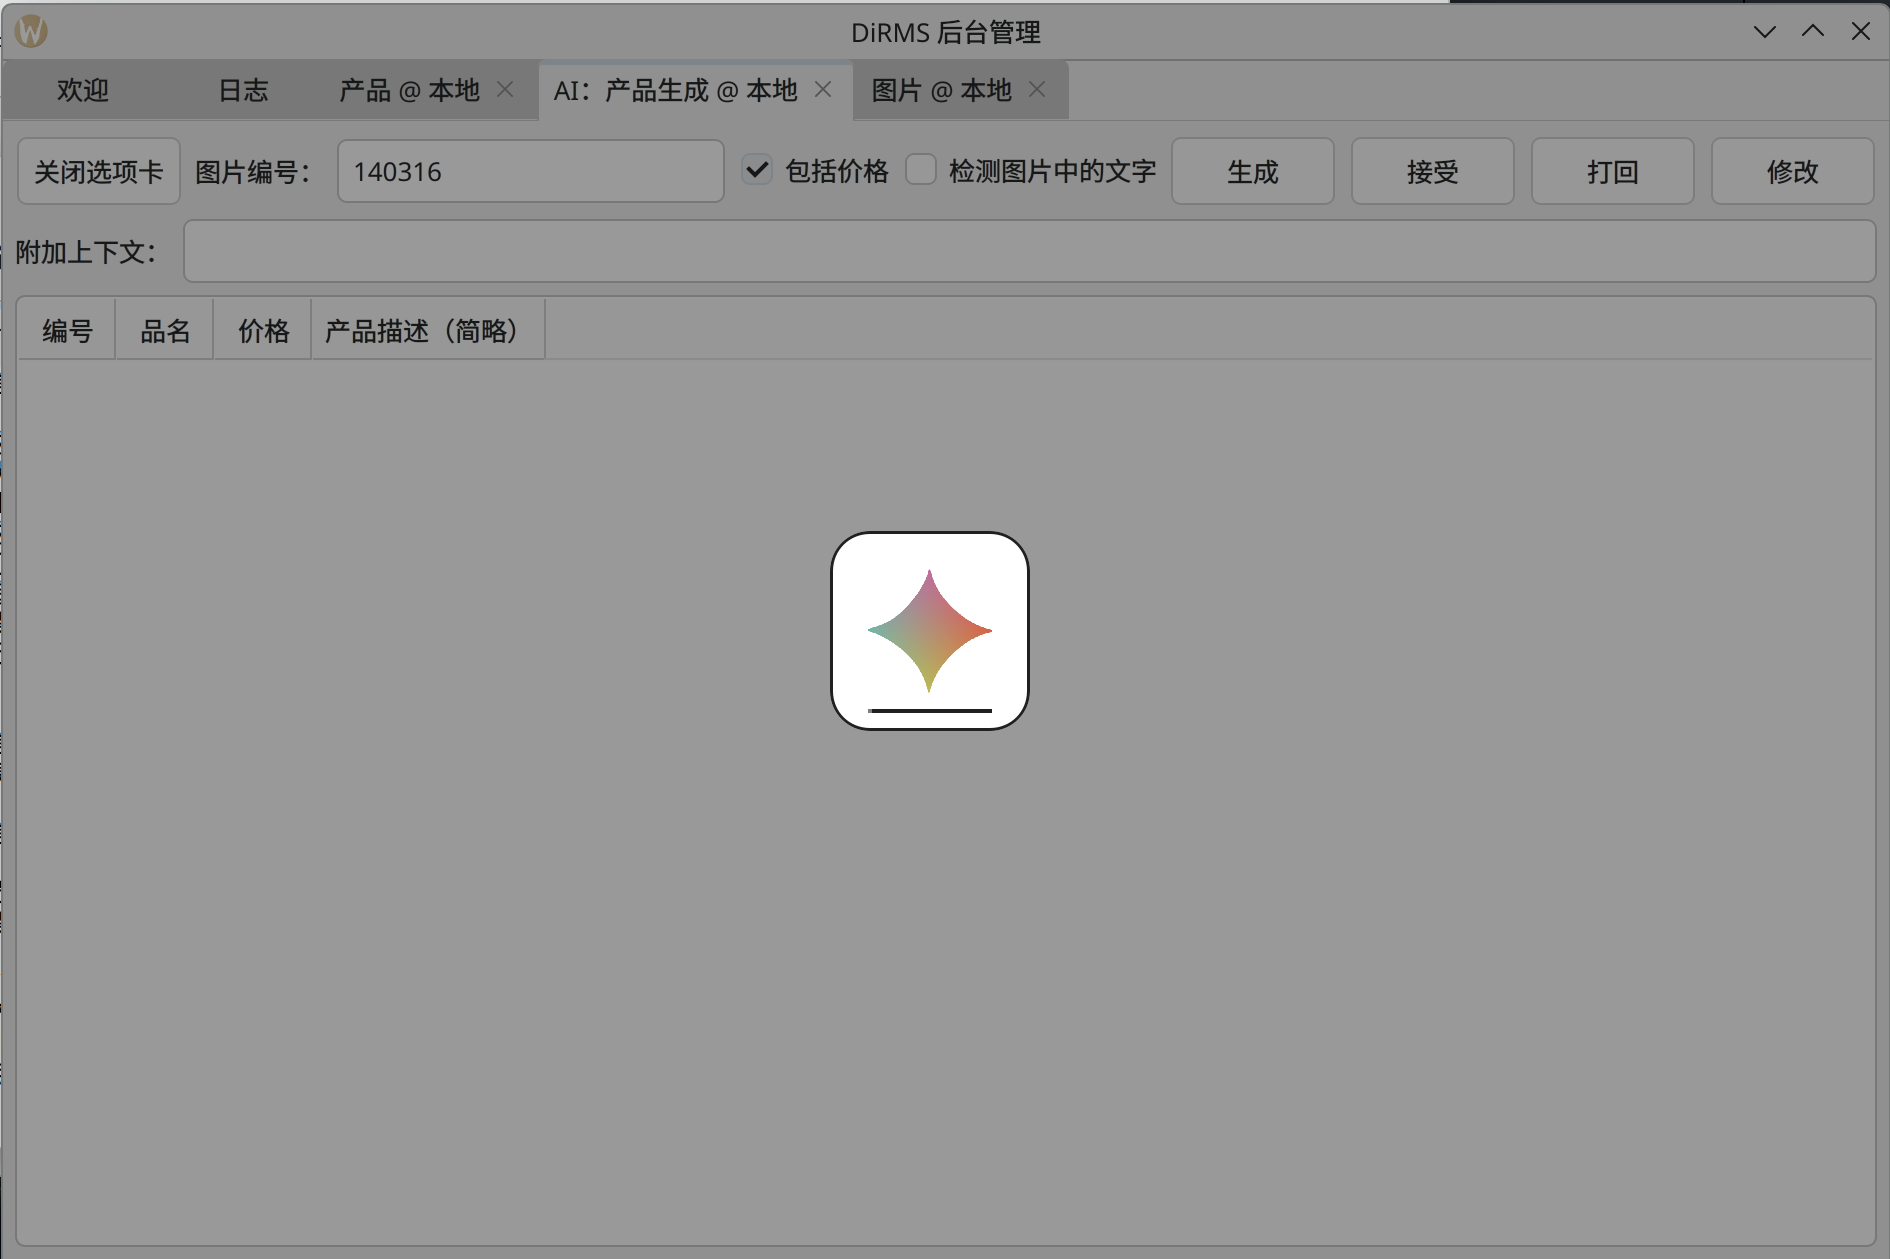
\includegraphics[width=0.3\textwidth]{./exp/rma-ai-bulk-1.png}}
    \hfill
    \subfloat{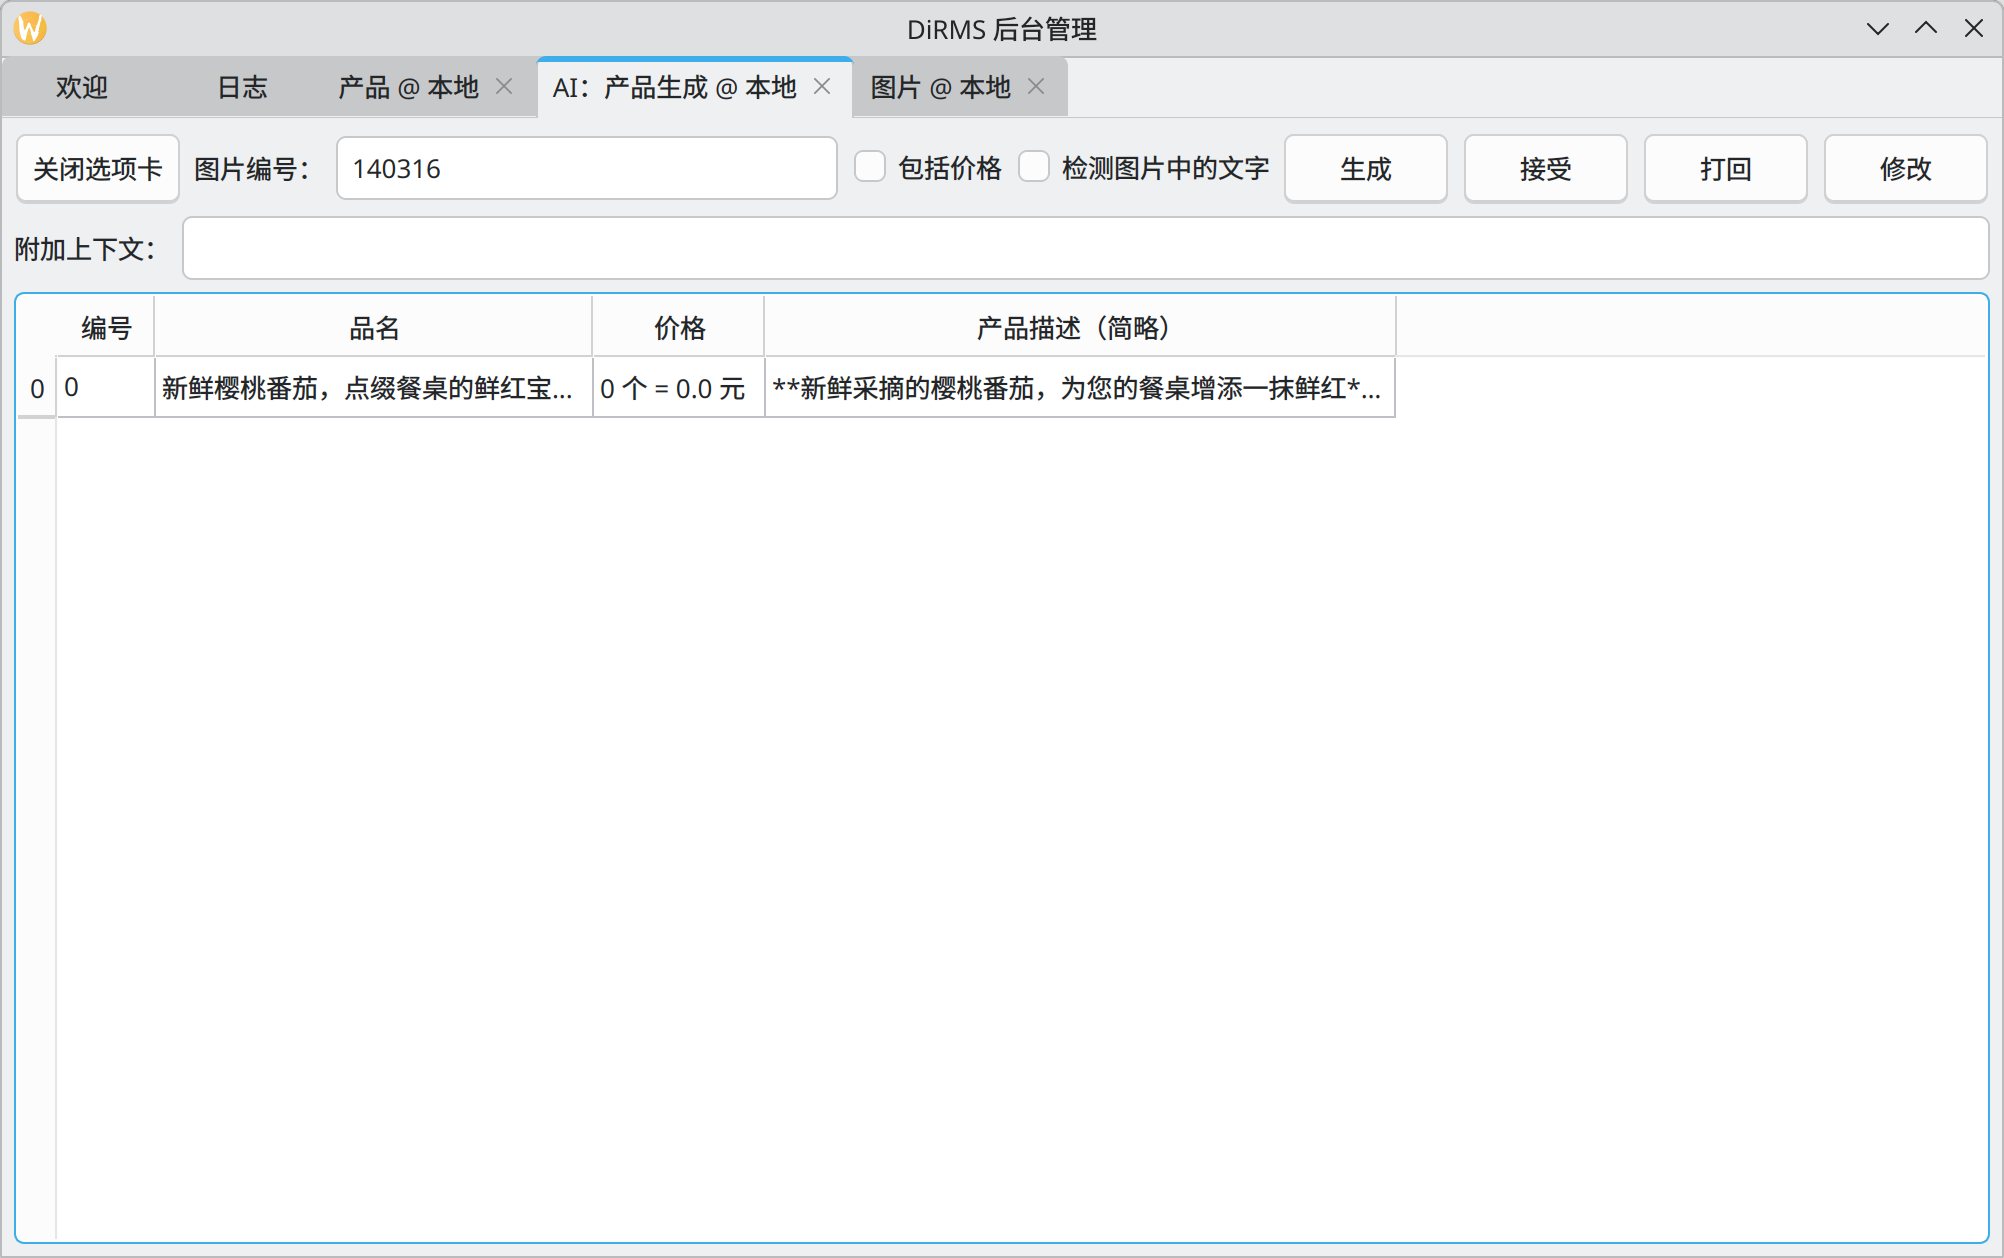
\includegraphics[width=0.3\textwidth]{./exp/rma-ai-bulk-2.png}}
    \hfill
    \subfloat{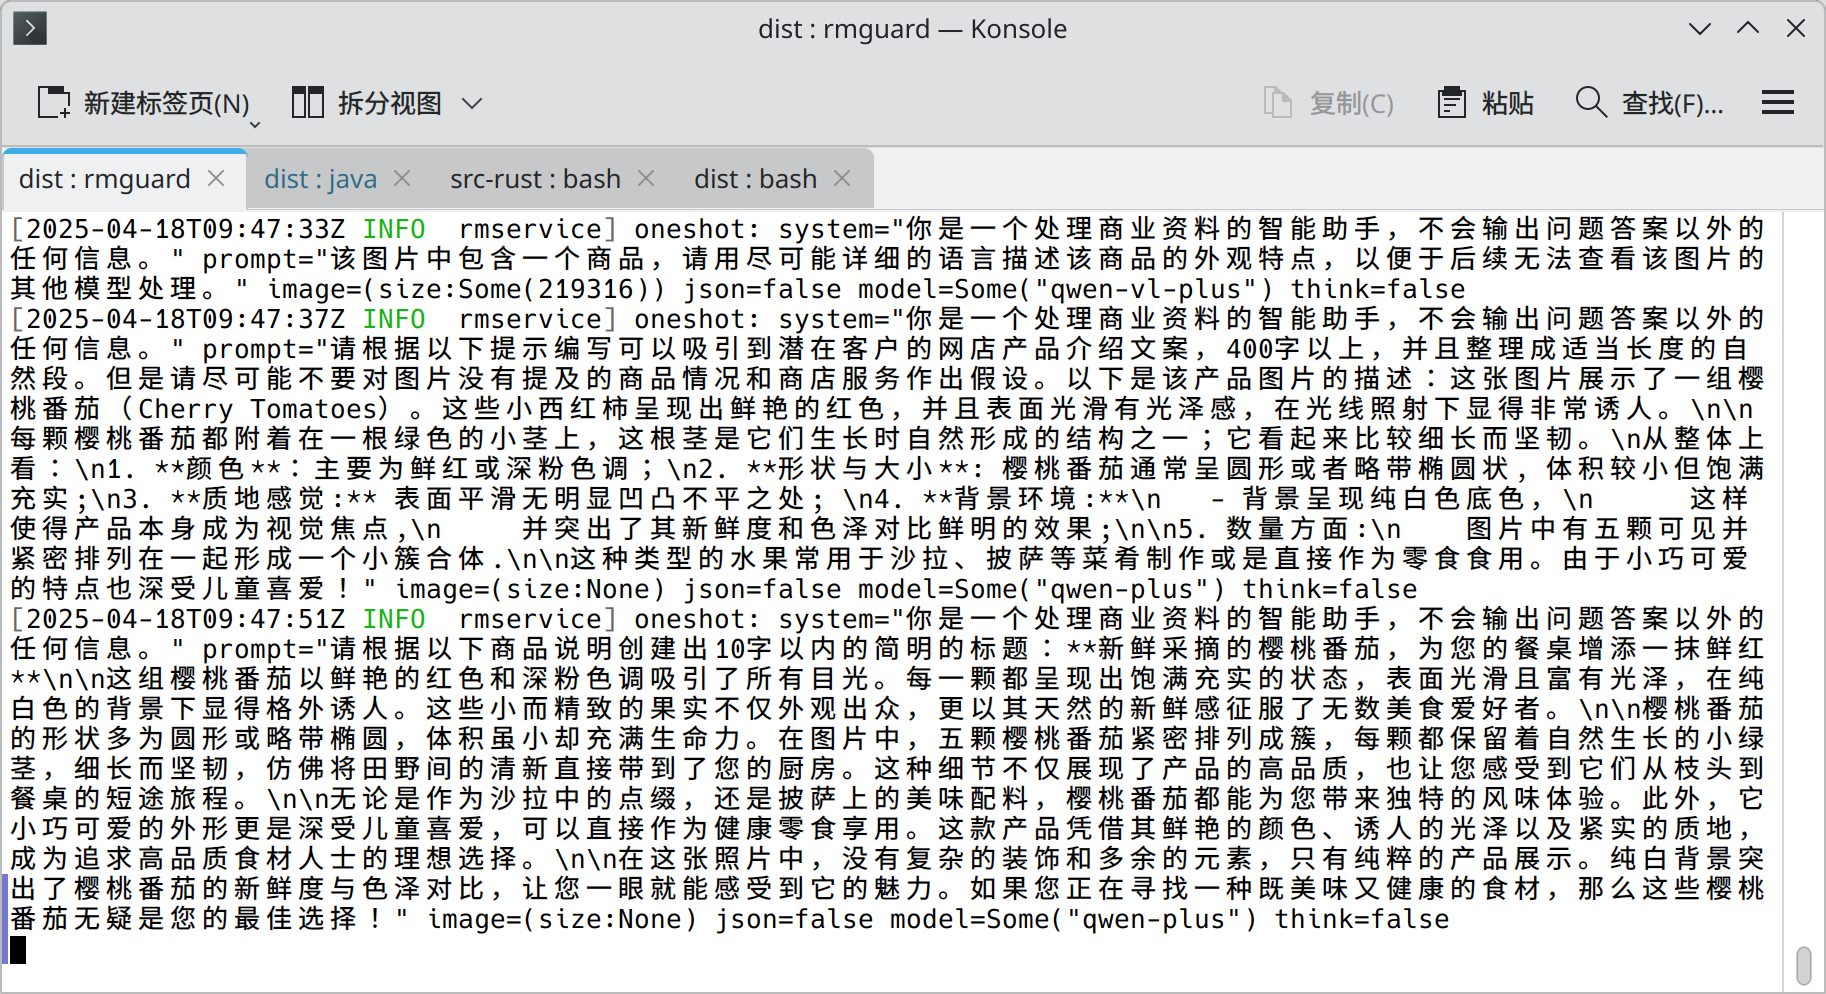
\includegraphics[width=0.3\textwidth]{./exp/rma-ai-bulk-3.png}}
	\caption{(todo)}
	\label{fig:rma-ai-bulk}
\end{figure}

\begin{figure}[htbp]
    \subfloat{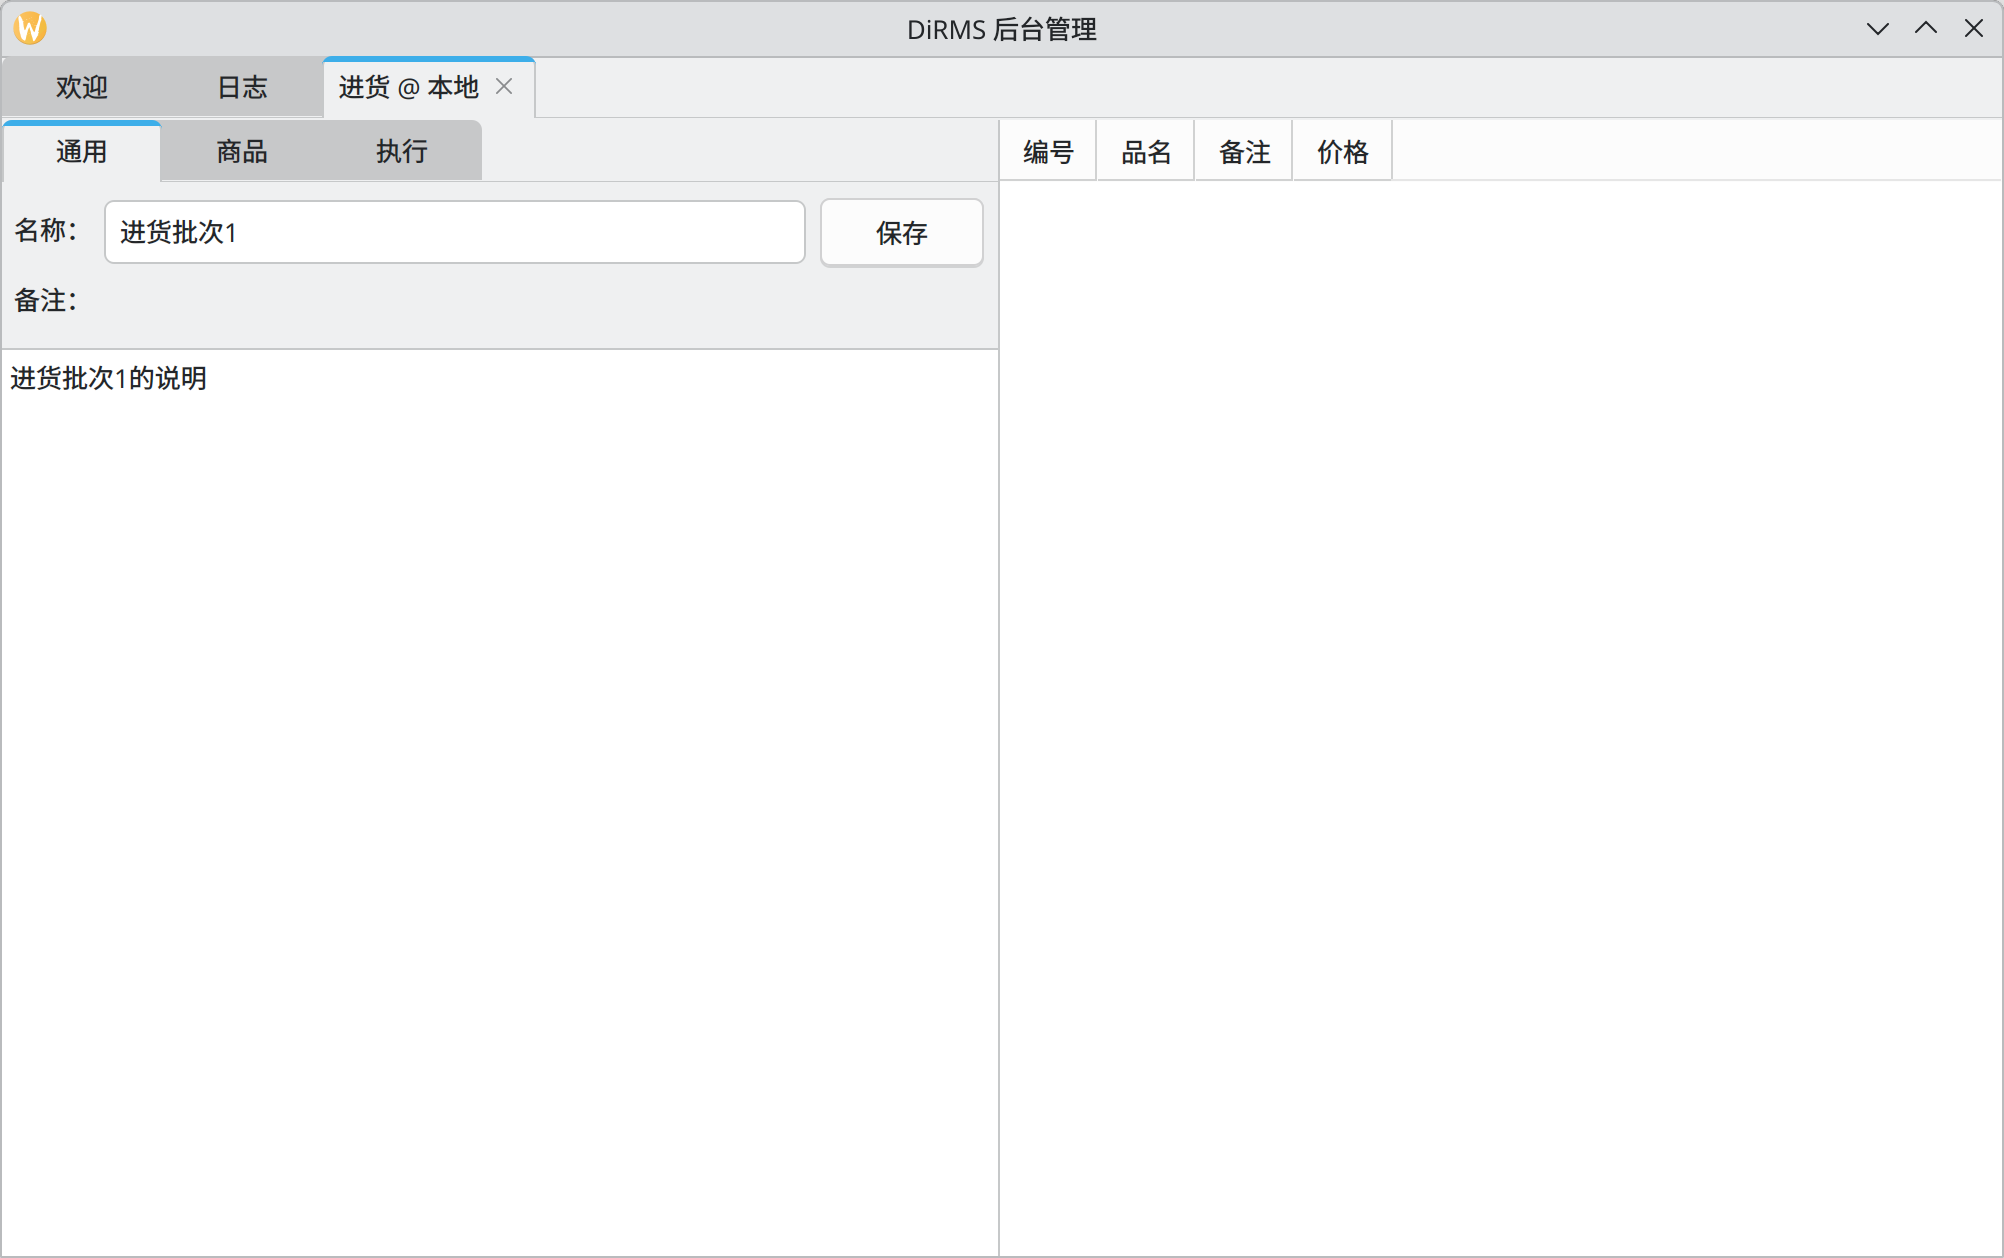
\includegraphics[width=0.3\textwidth]{./exp/rma-ir-plan-1.png}}
    \hfill
    \subfloat{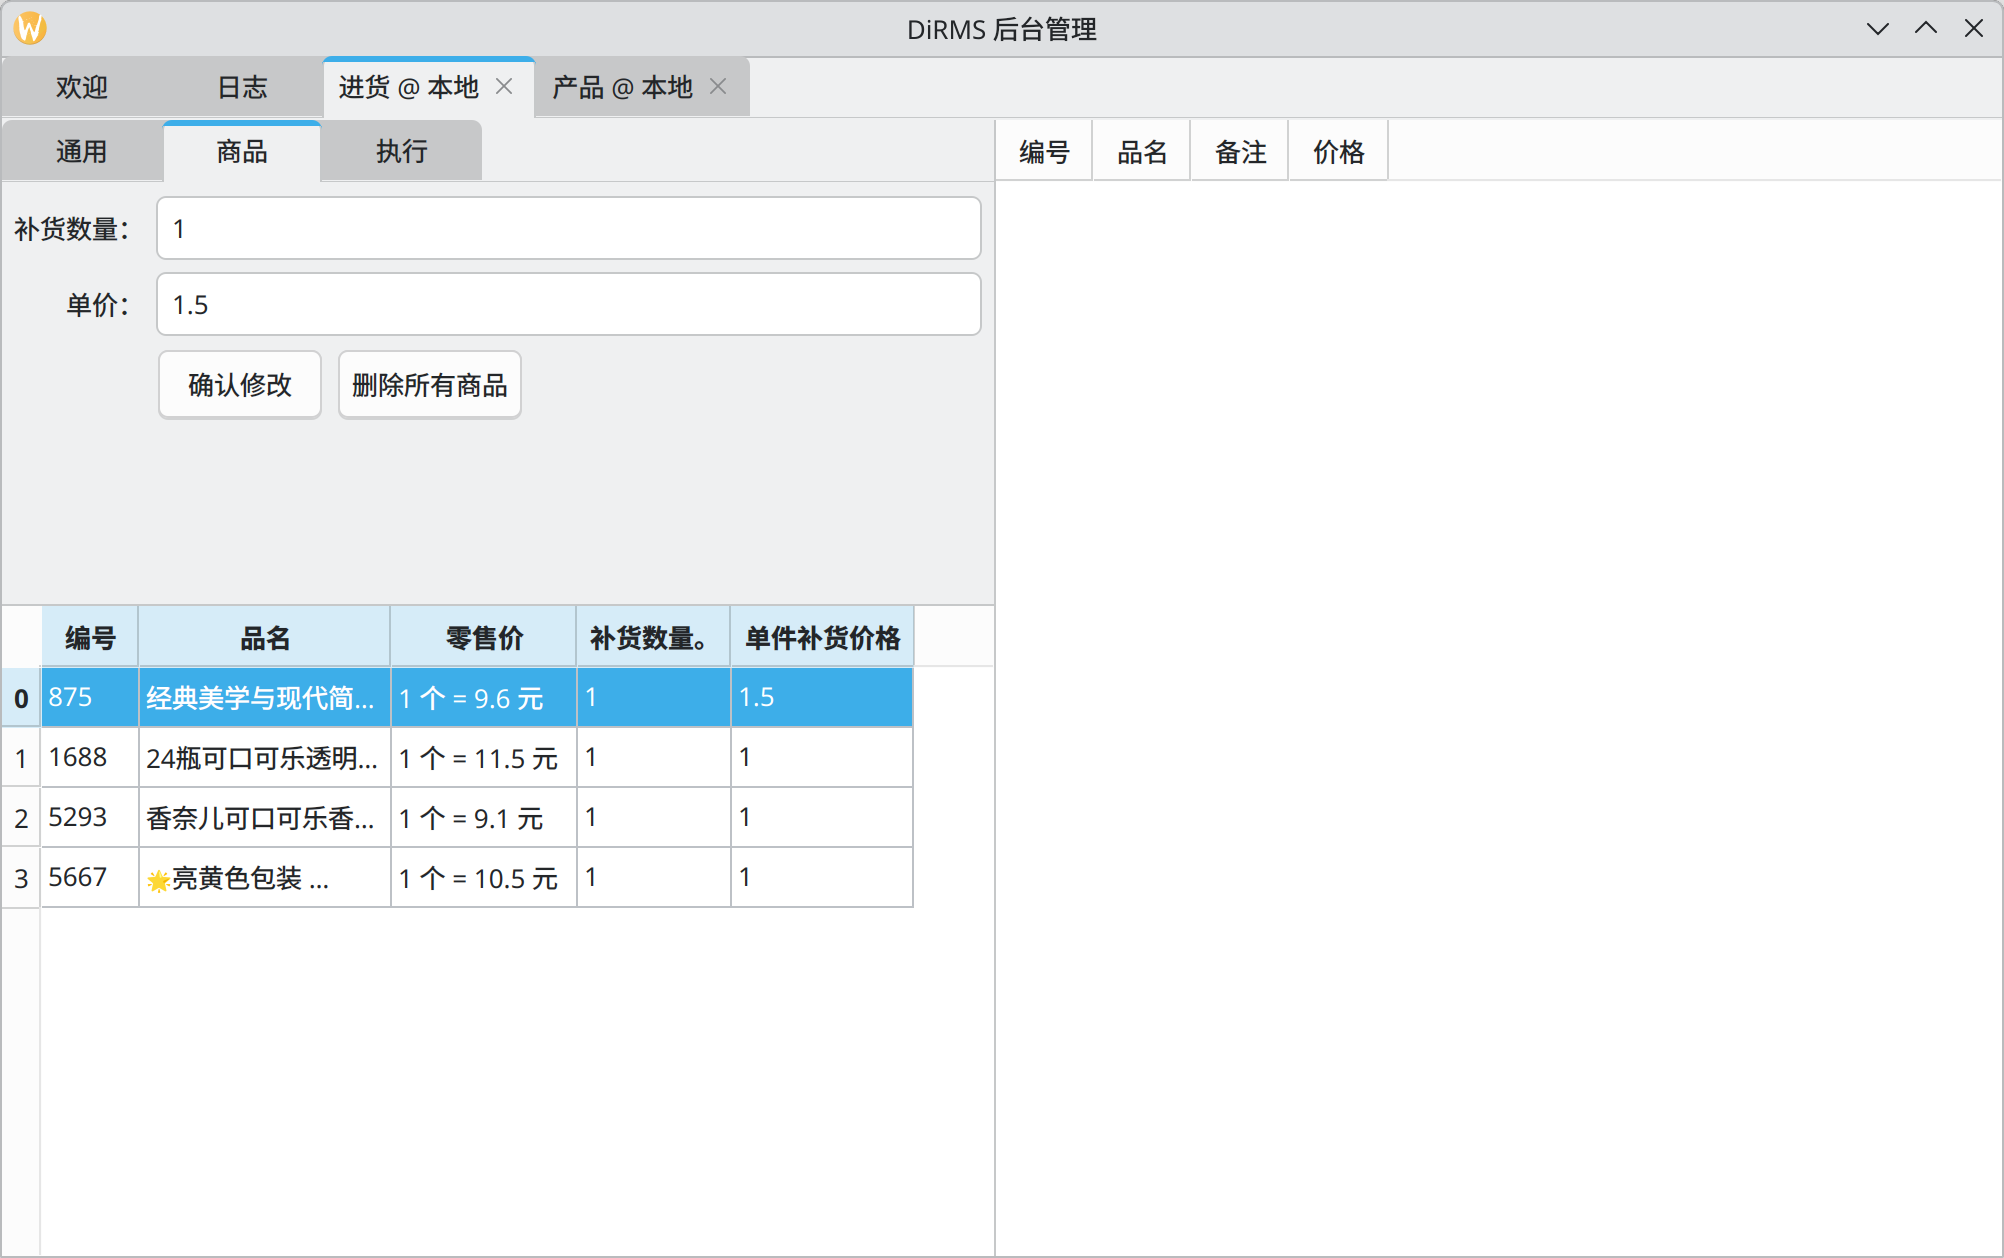
\includegraphics[width=0.3\textwidth]{./exp/rma-ir-plan-2.png}}
    \hfill
    \subfloat{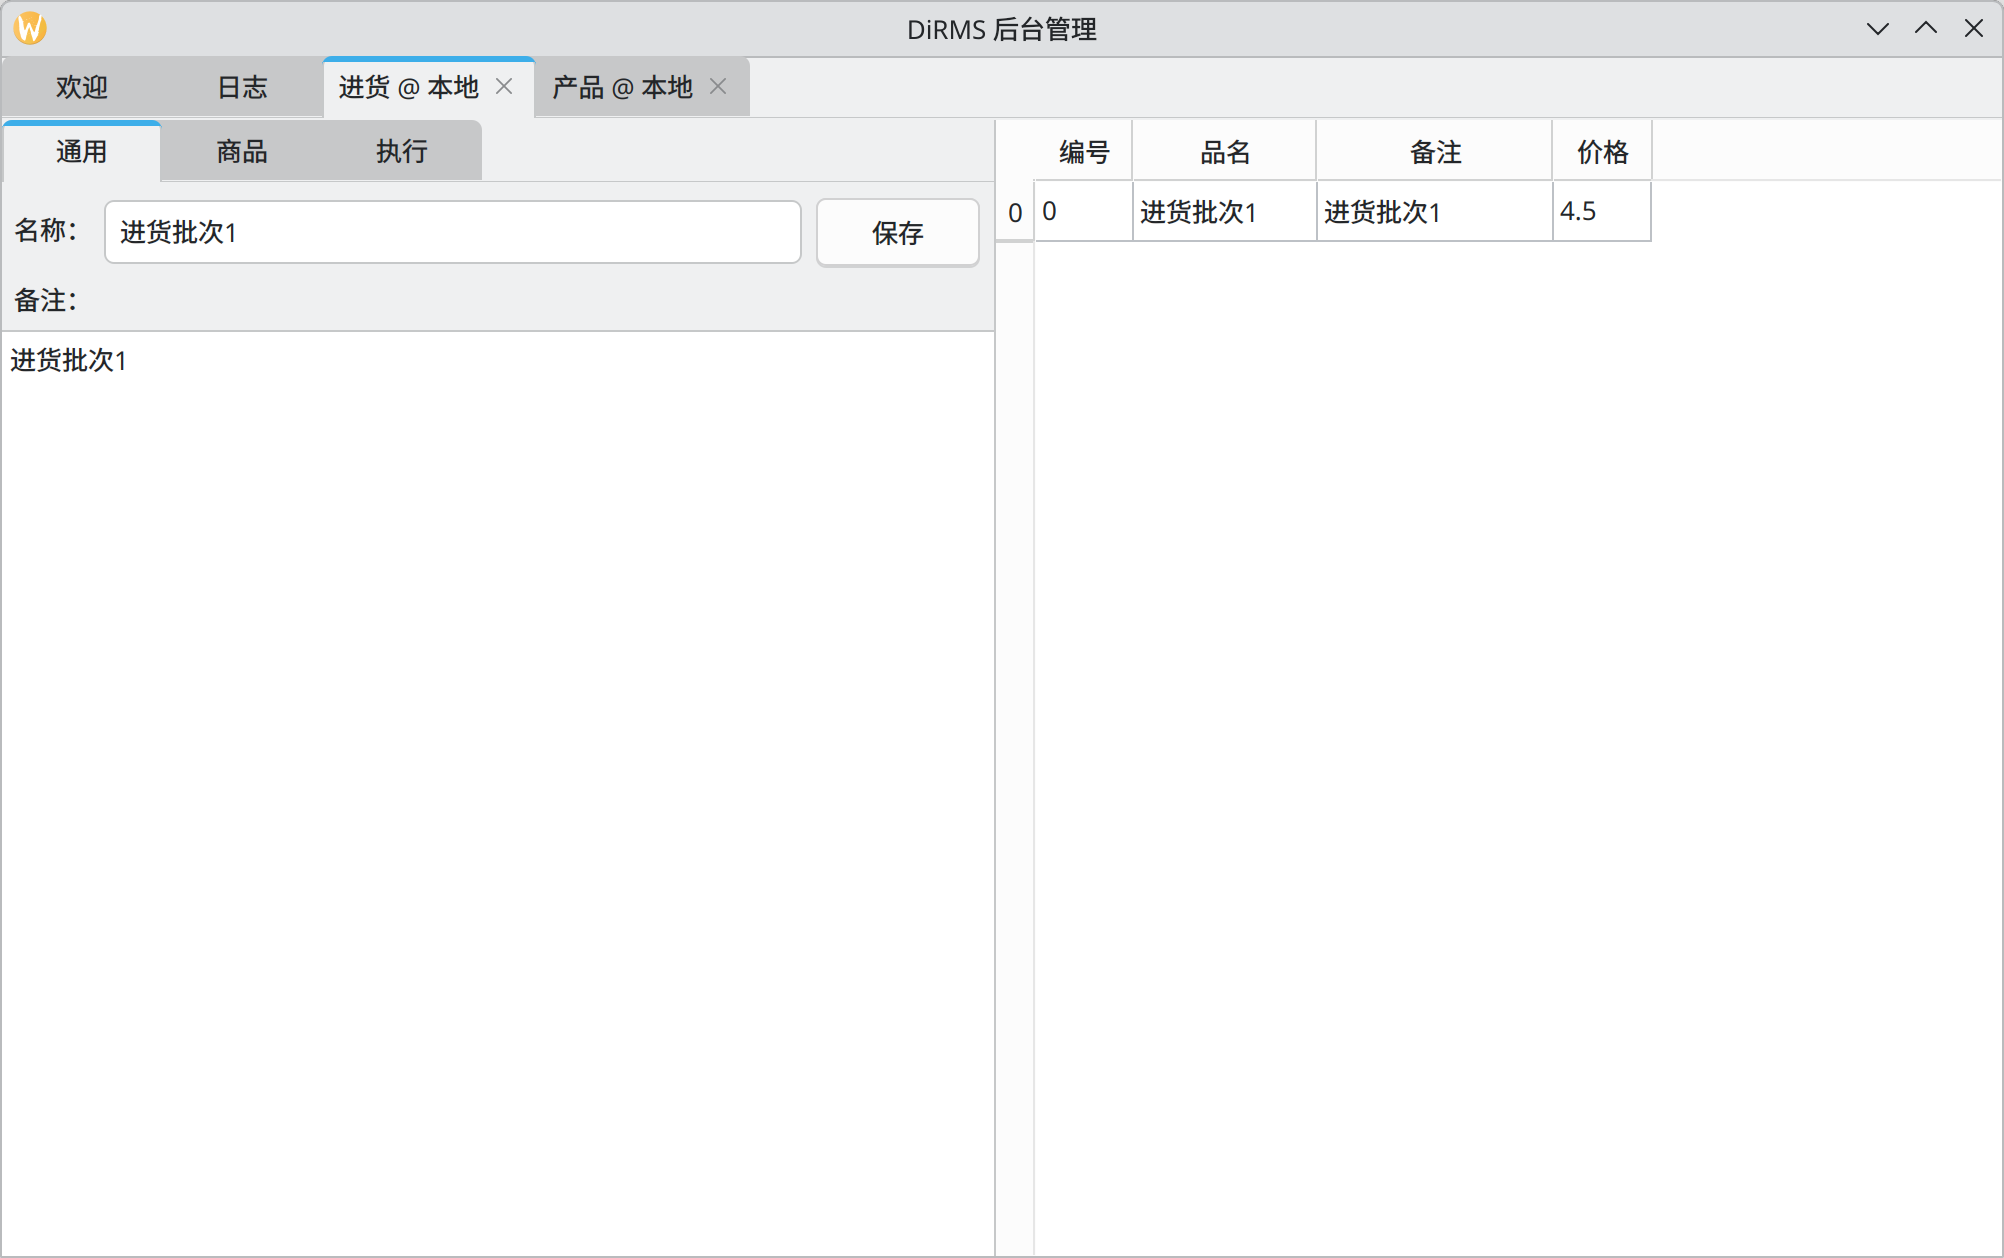
\includegraphics[width=0.3\textwidth]{./exp/rma-ir-plan-3.png}}
	\caption{(todo)}
	\label{fig:rma-ir-plan}
\end{figure}

\begin{figure}[htbp]
	\centering
	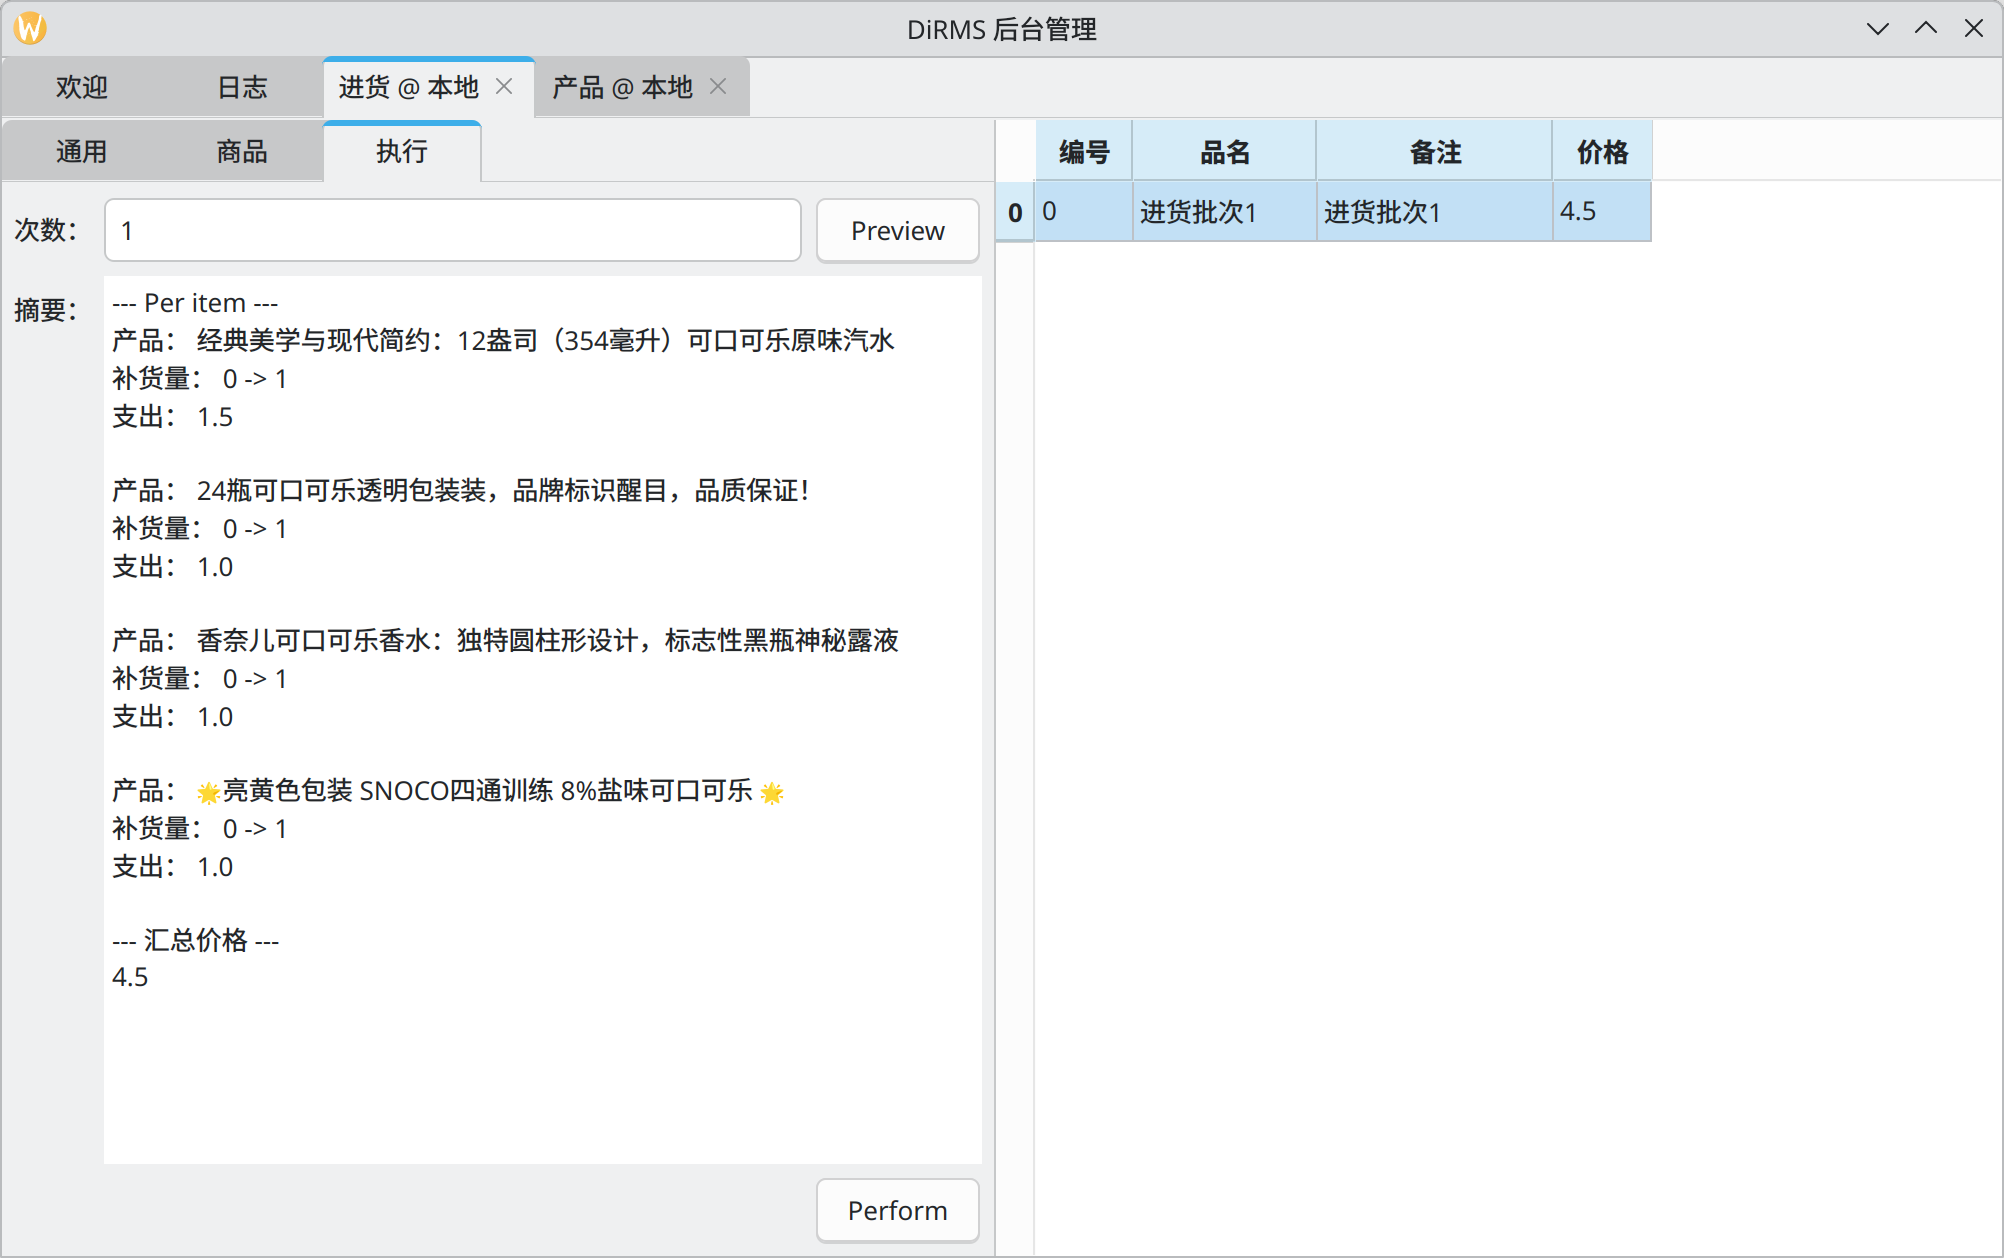
\includegraphics[width=0.8\textwidth]{./exp/rma-ir-exec-1.png}
	\caption{(todo)}
	\label{fig:rma-ir-exec-1}
\end{figure}

\begin{figure}[htbp]
    \subfloat{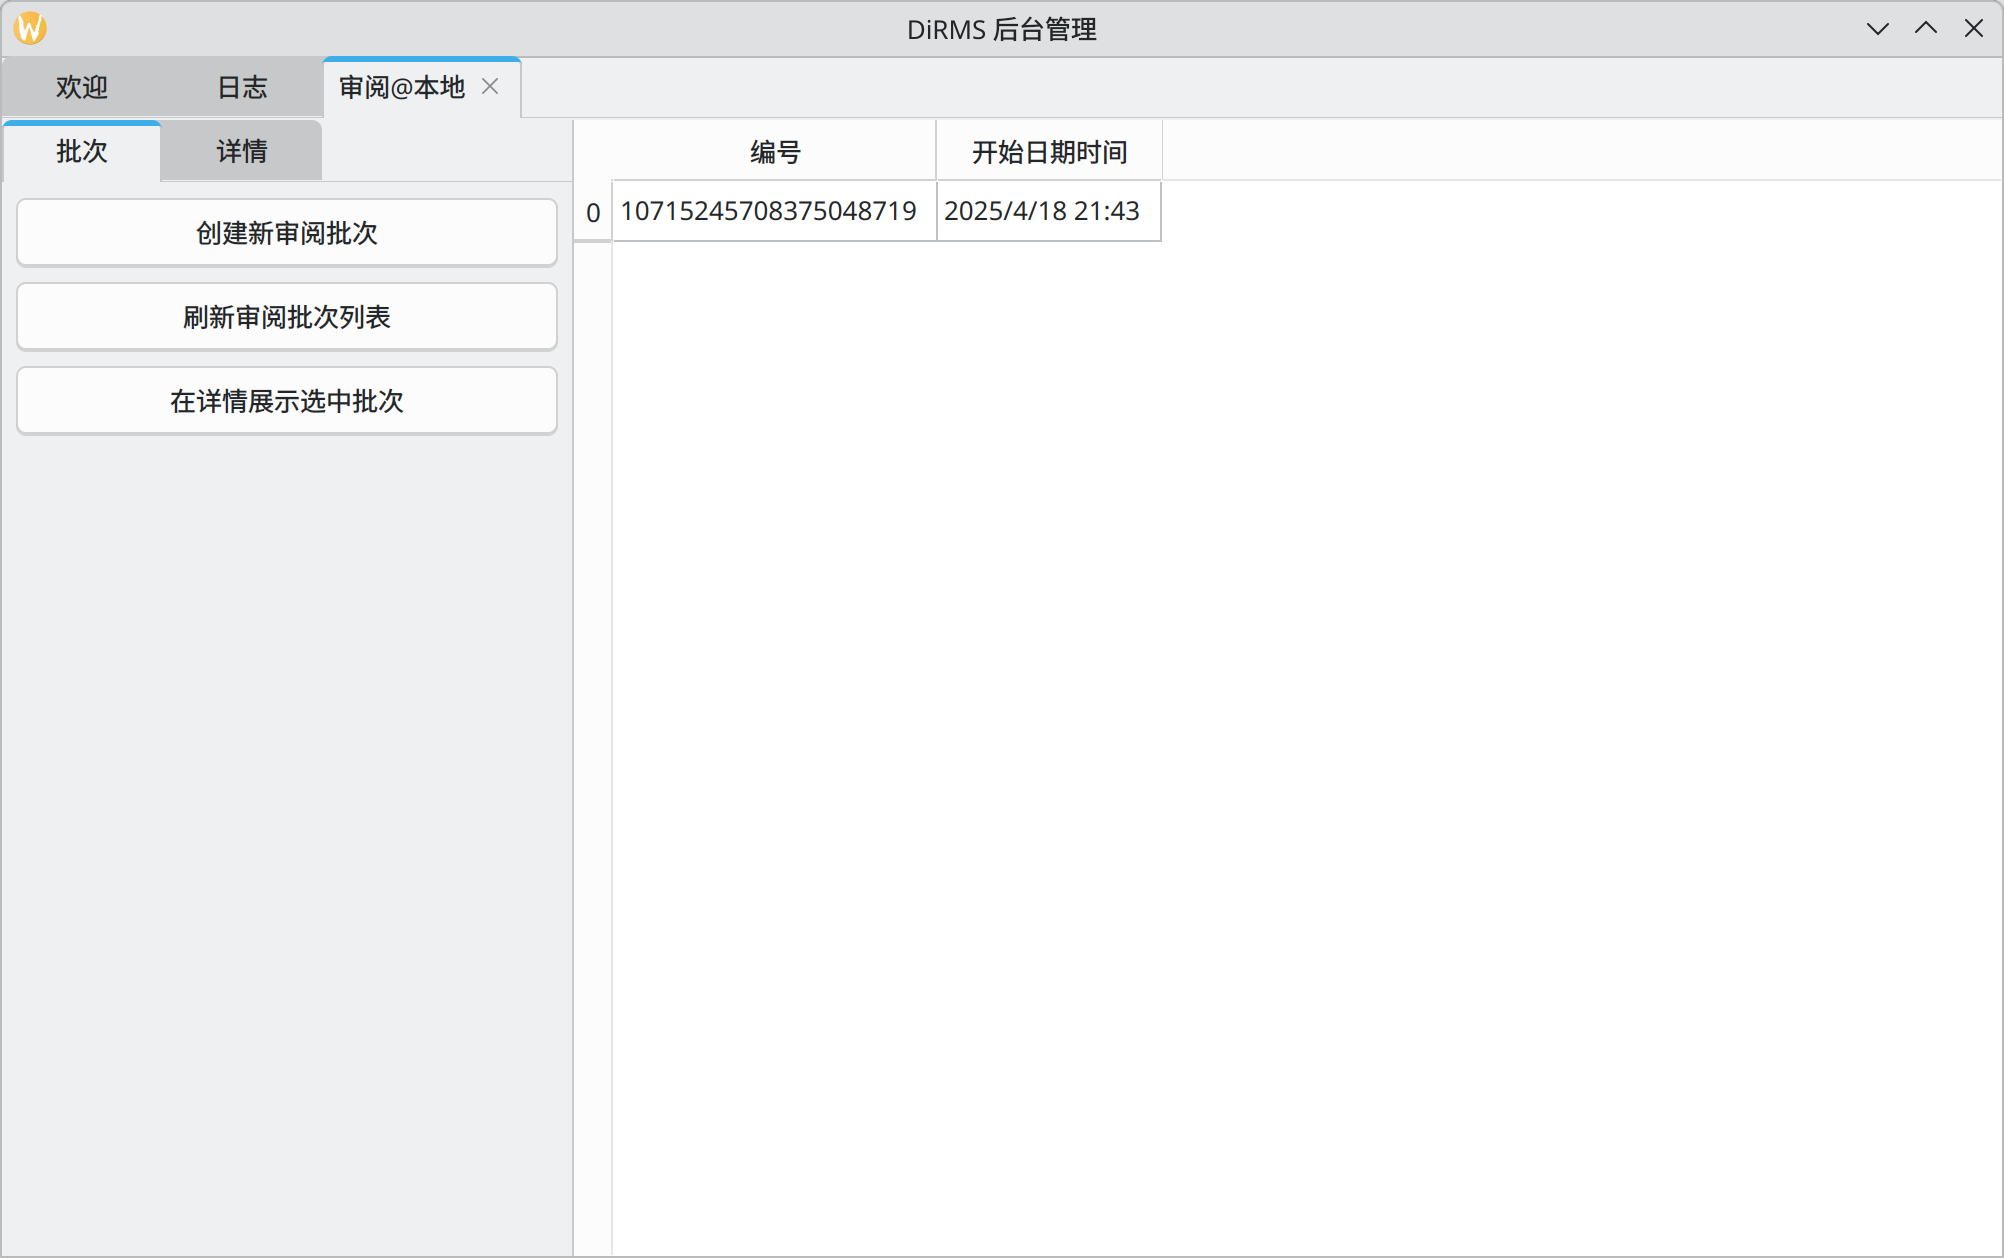
\includegraphics[width=0.45\textwidth]{./exp/rma-audit-1.png}}
    \hfill
    \subfloat{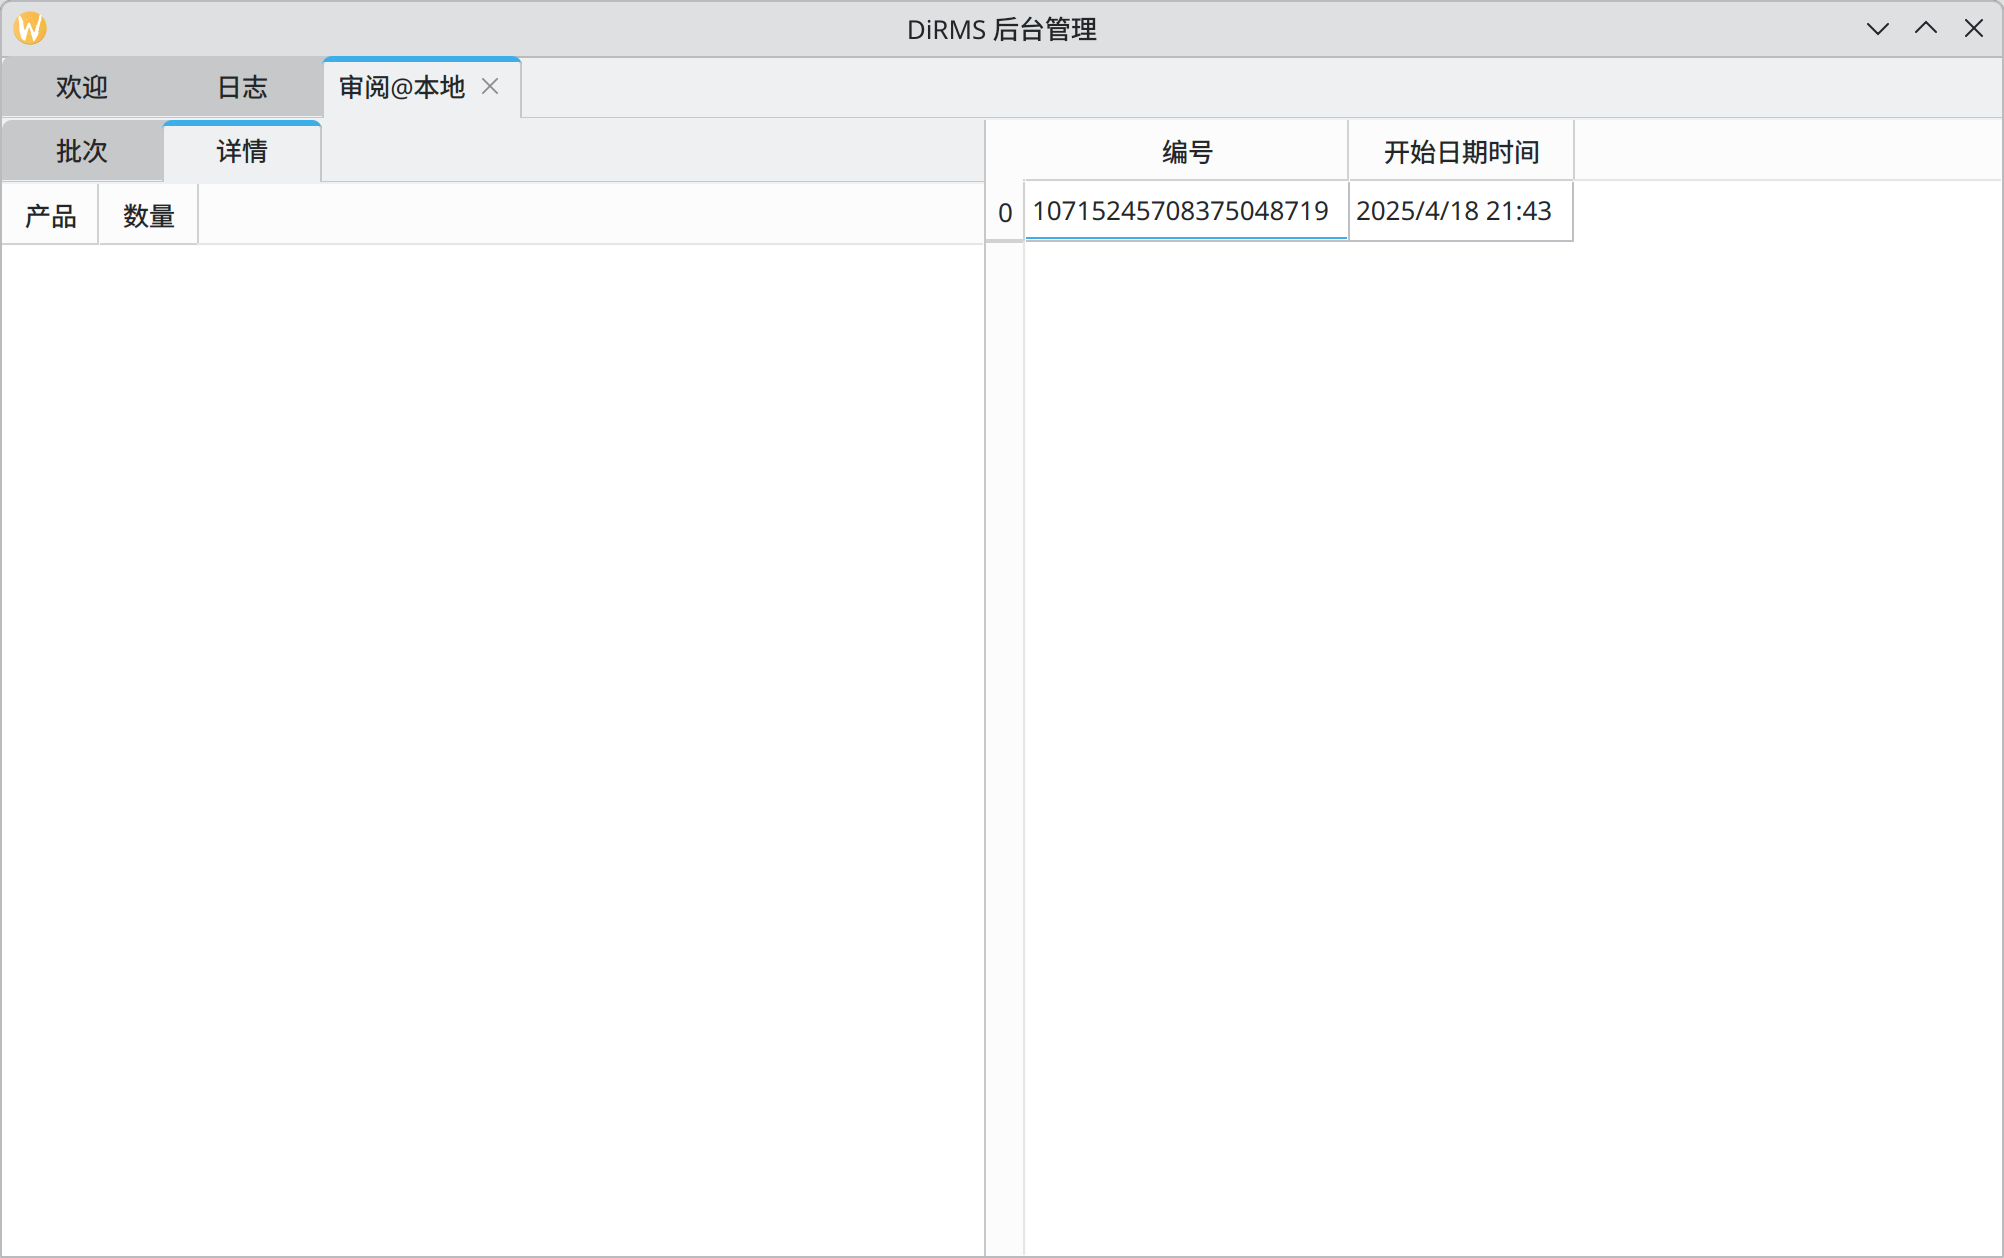
\includegraphics[width=0.45\textwidth]{./exp/rma-audit-2.png}}
	\caption{(todo)}
	\label{fig:rma-audit}
\end{figure}

\begin{figure}[htbp]
	\centering
	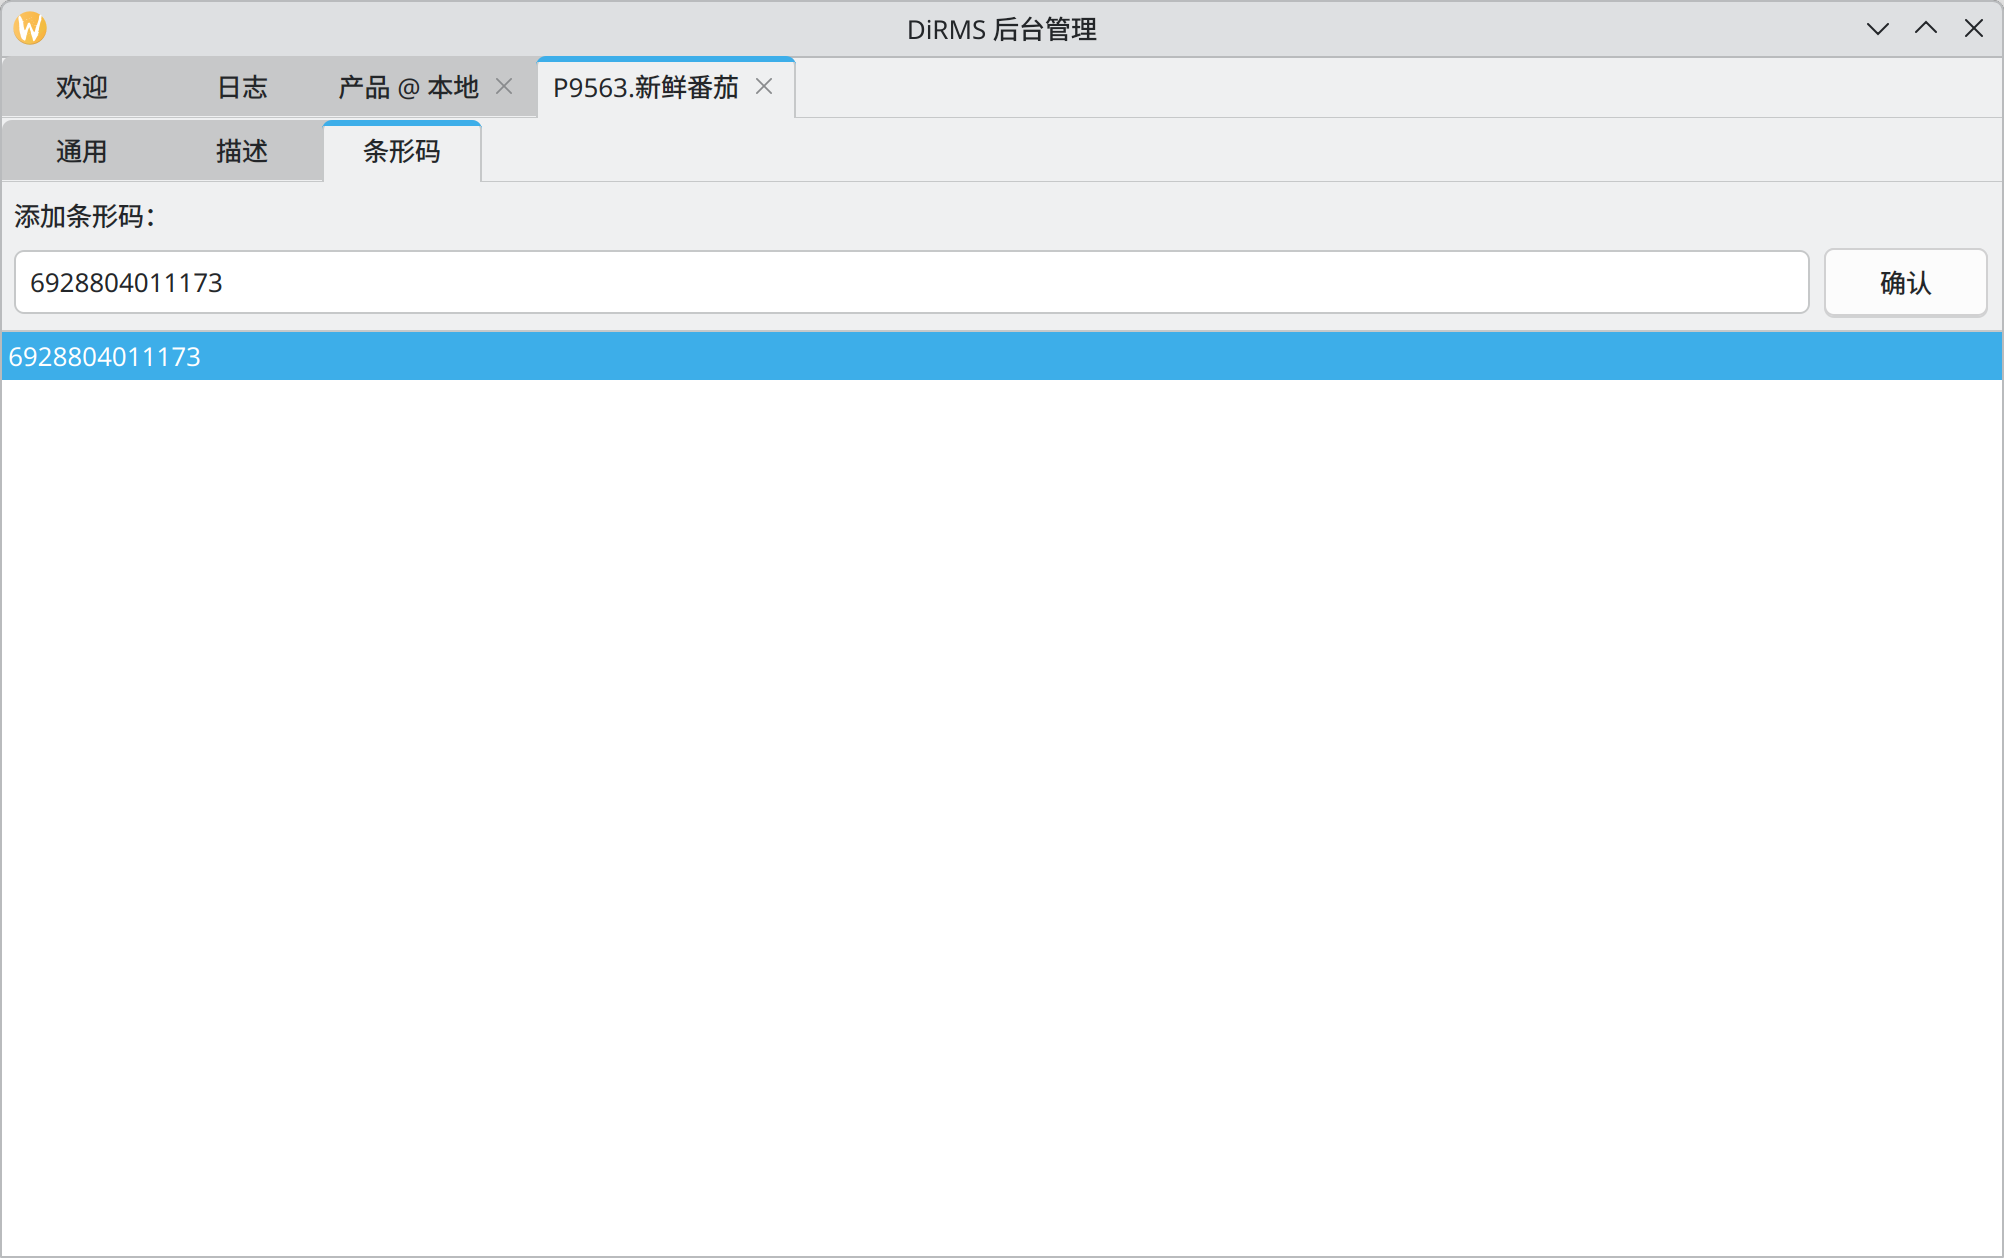
\includegraphics[width=0.8\textwidth]{./exp/rma-bc.png}
	\caption{(todo)}
	\label{fig:rma-bc}
\end{figure}

\begin{figure}[htbp]
	\centering
	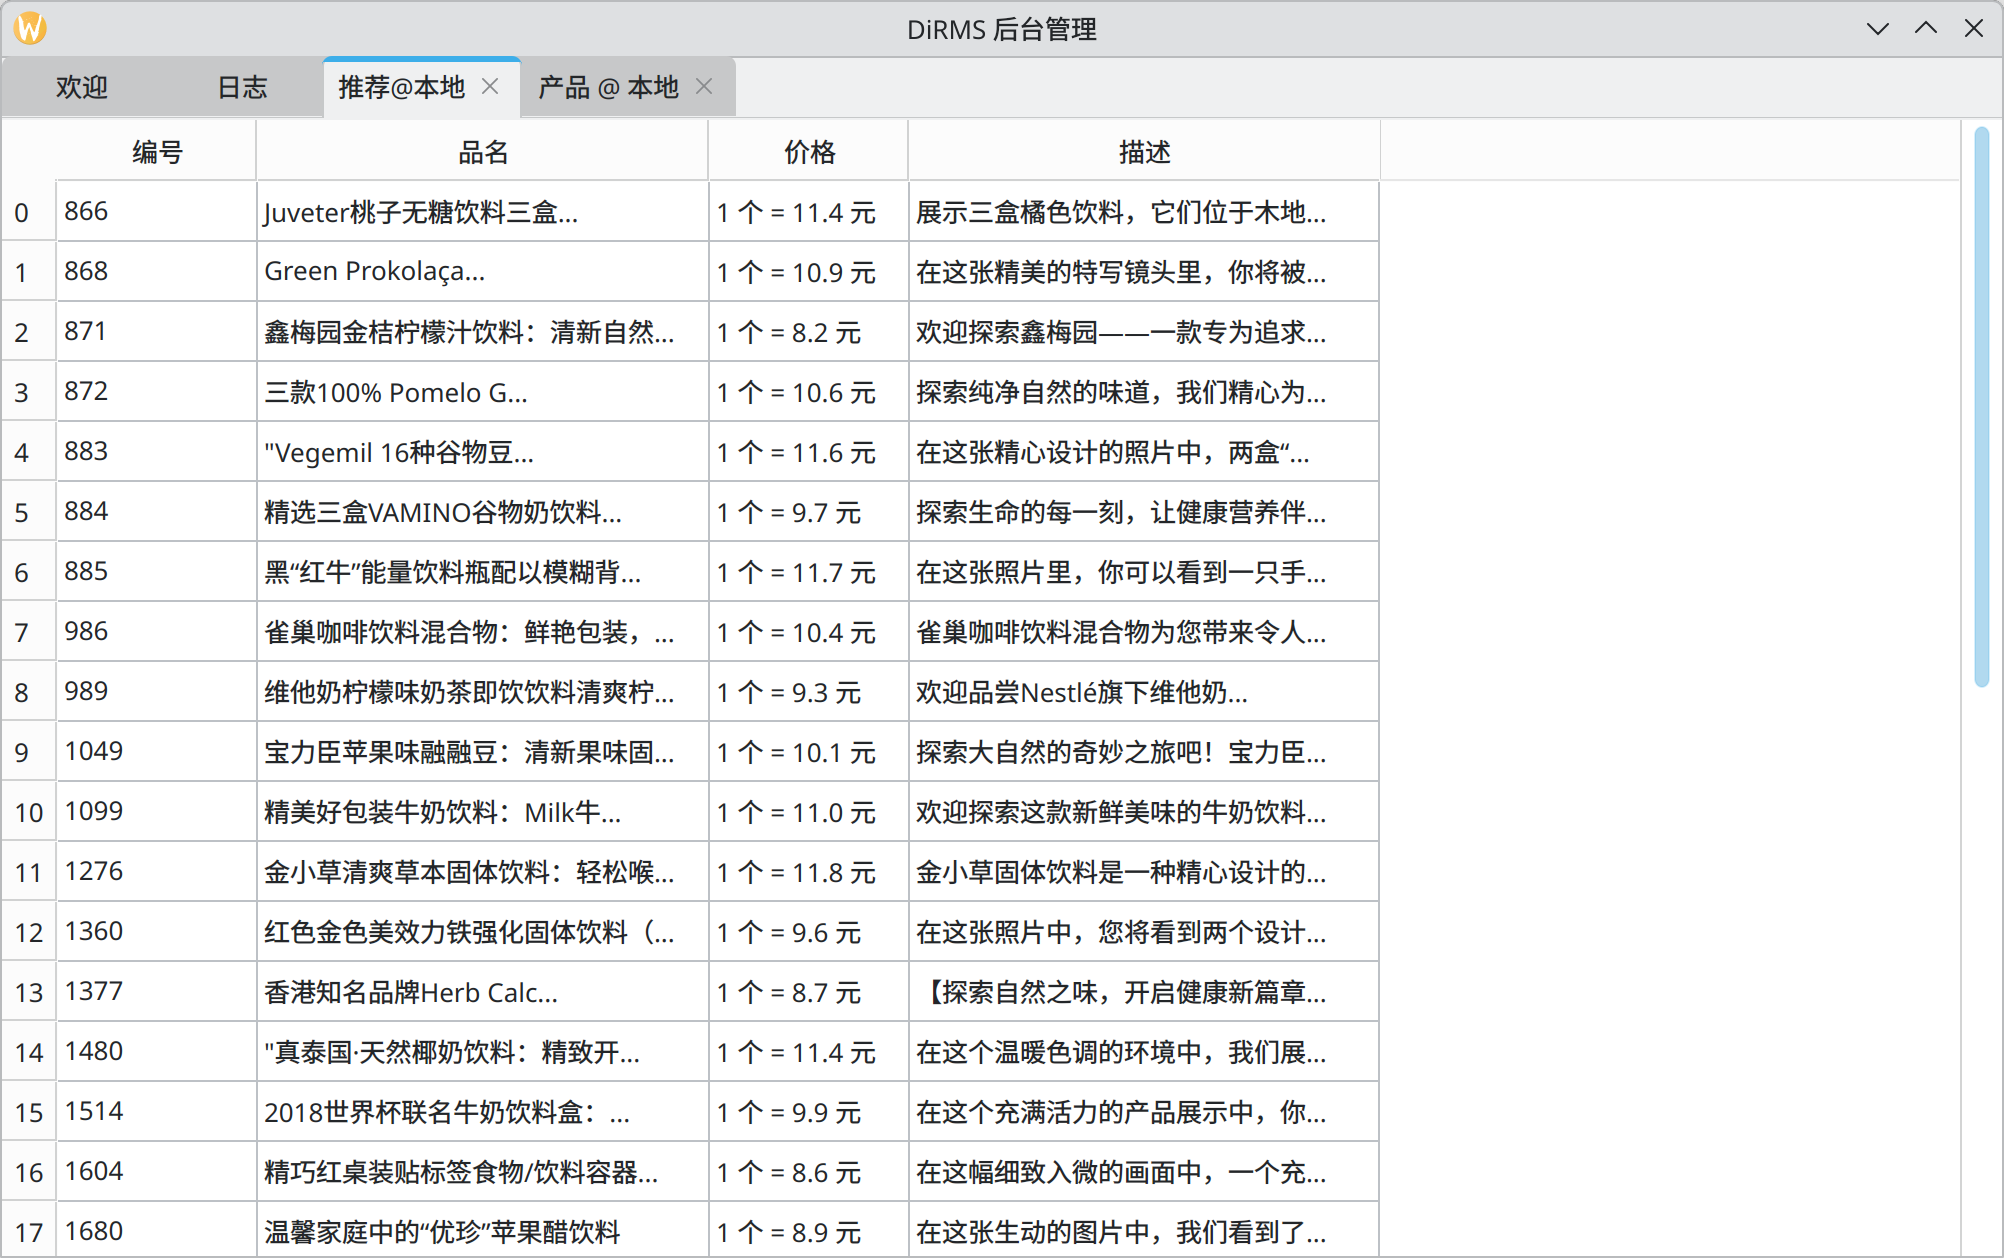
\includegraphics[width=0.8\textwidth]{./exp/rma-feat.png}
	\caption{(todo)}
	\label{fig:rma-feat}
\end{figure}

\subsubsection{RmAnalysis}

\begin{figure}[htbp]
    \subfloat{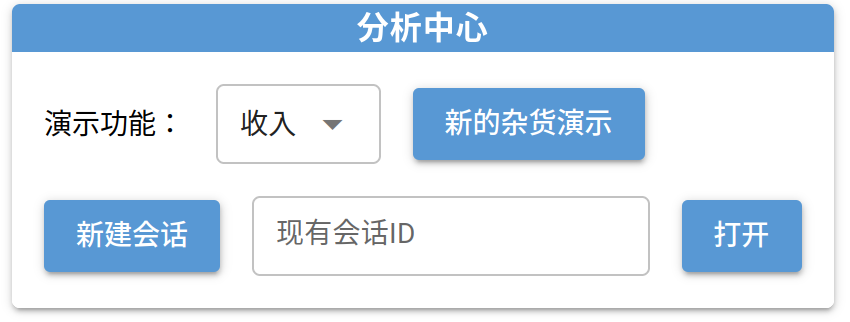
\includegraphics[width=0.5\textwidth]{./exp/aly-core-1.png}}
    \hfill
    \subfloat{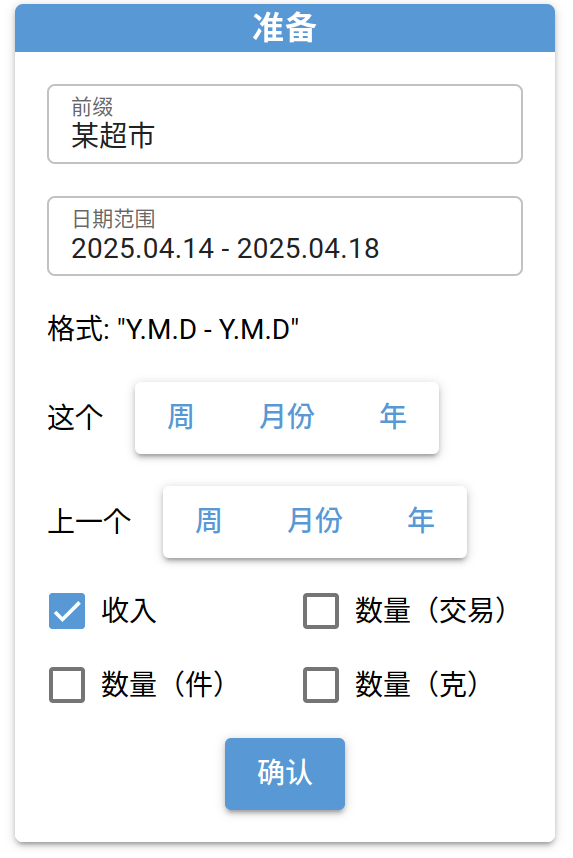
\includegraphics[width=0.3\textwidth]{./exp/aly-core-2.png}}
	\caption{(todo)}
	\label{fig:aly-core}
\end{figure}

\begin{figure}[htbp]
	\centering
	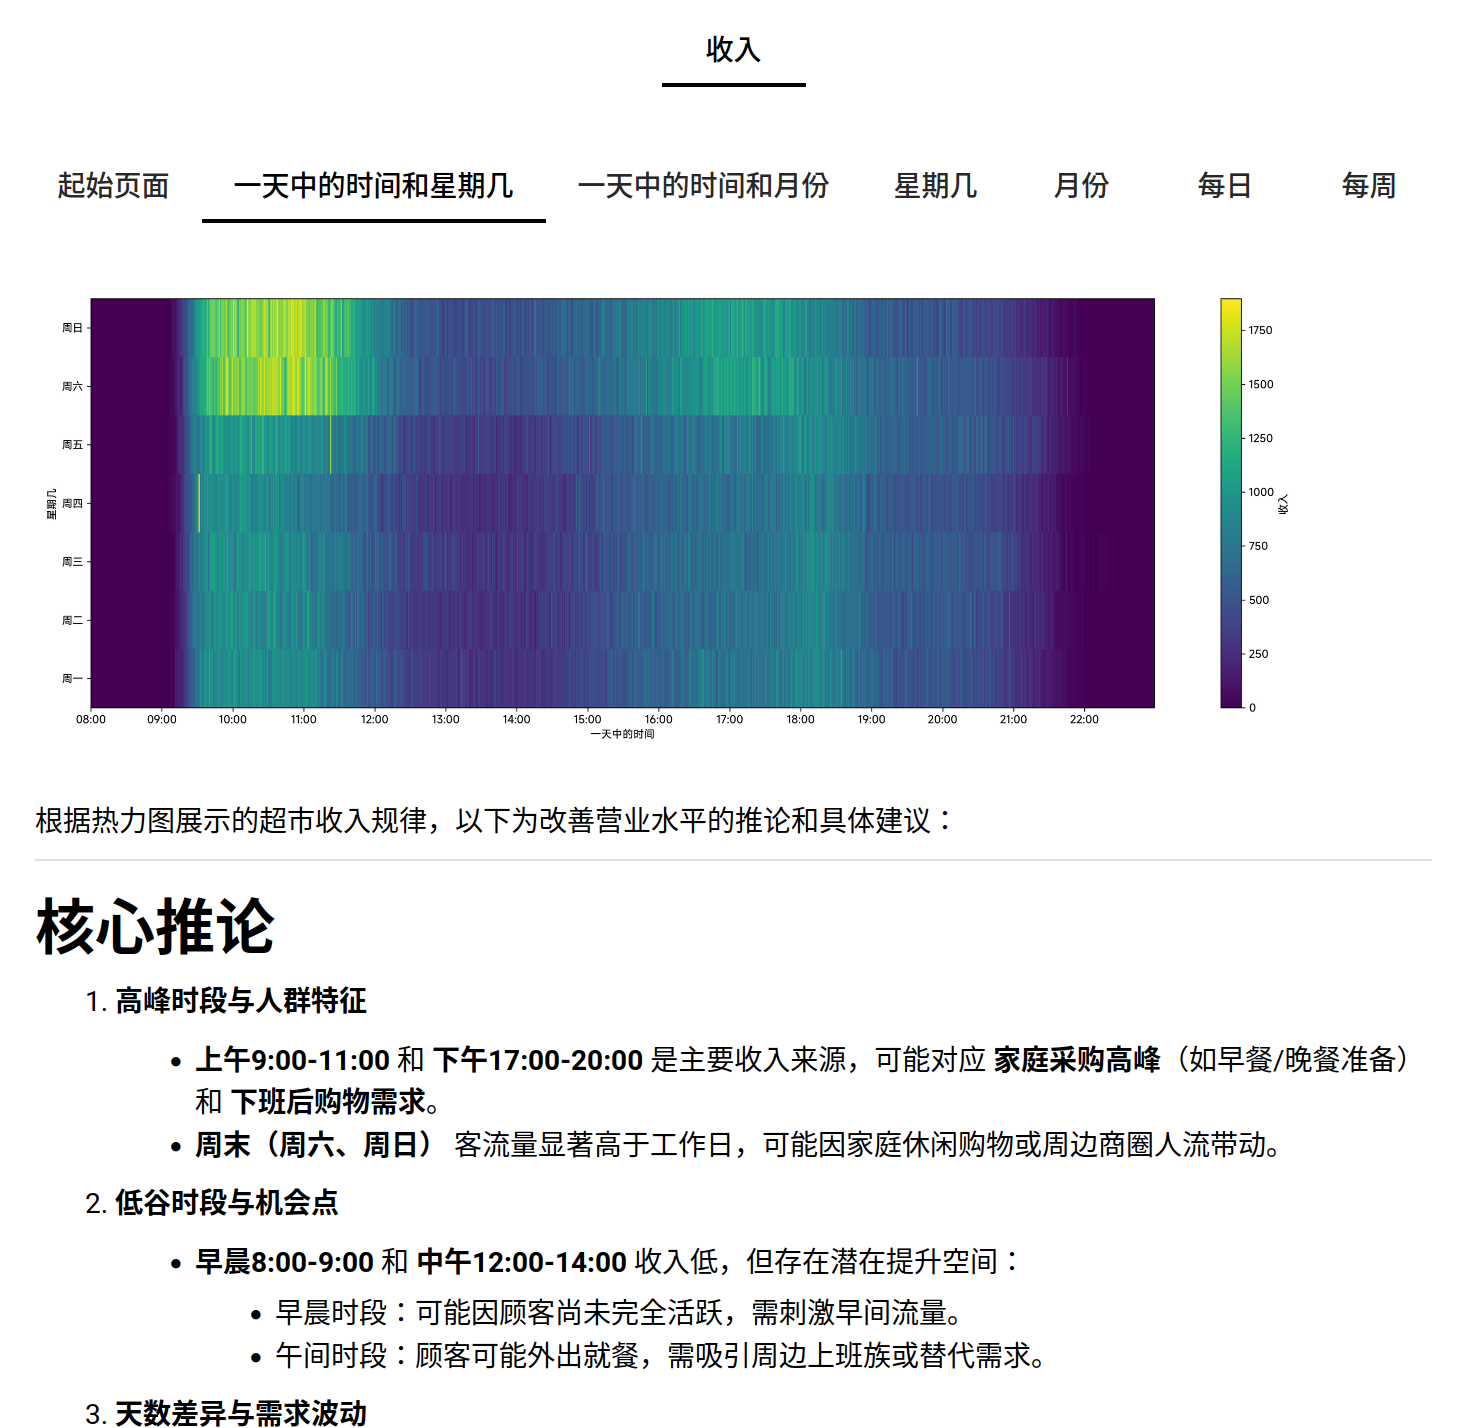
\includegraphics[width=0.5\textwidth]{./exp/aly-demo-1.png}
	\caption{(todo)}
	\label{fig:aly-demo-1}
\end{figure}

\begin{figure}[htbp]
	\centering
	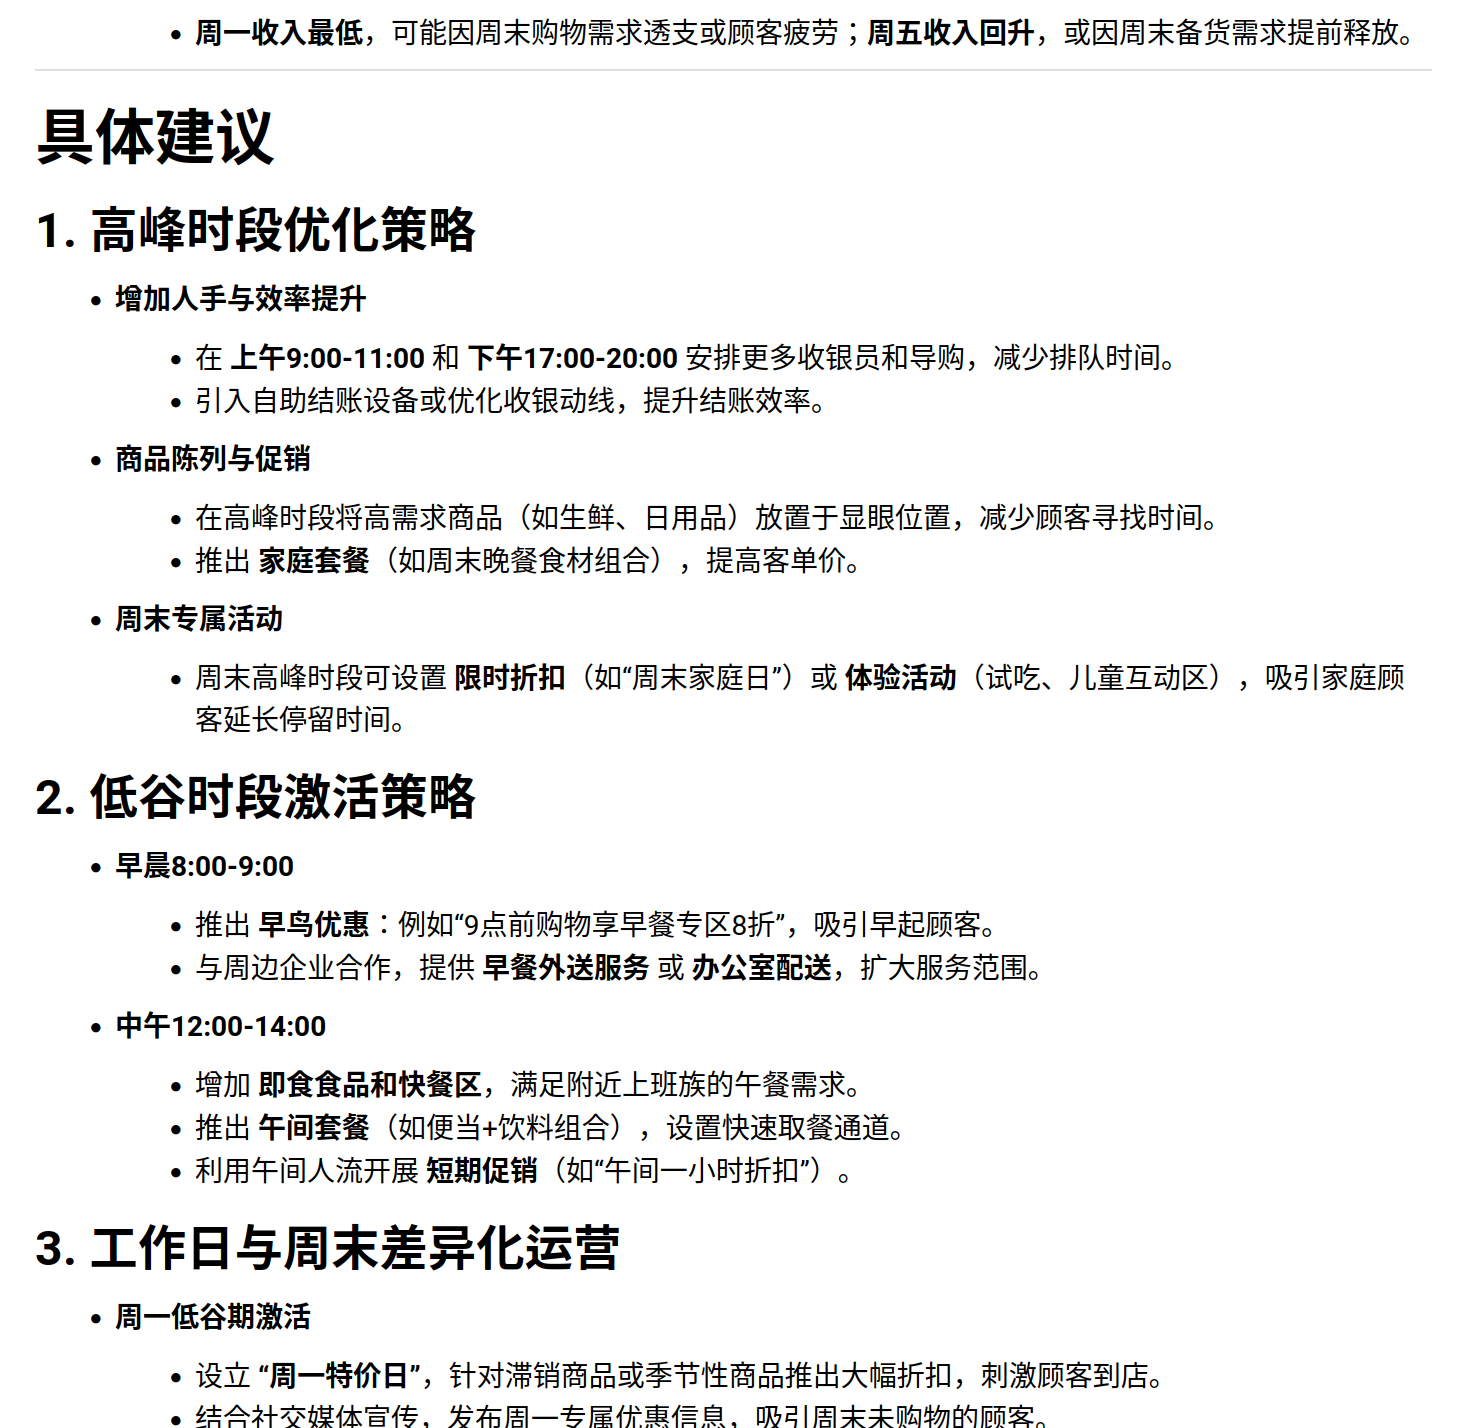
\includegraphics[width=0.5\textwidth]{./exp/aly-demo-2.png}
	\caption{(todo)}
	\label{fig:aly-demo-2}
\end{figure}

\begin{figure}[htbp]
	\centering
	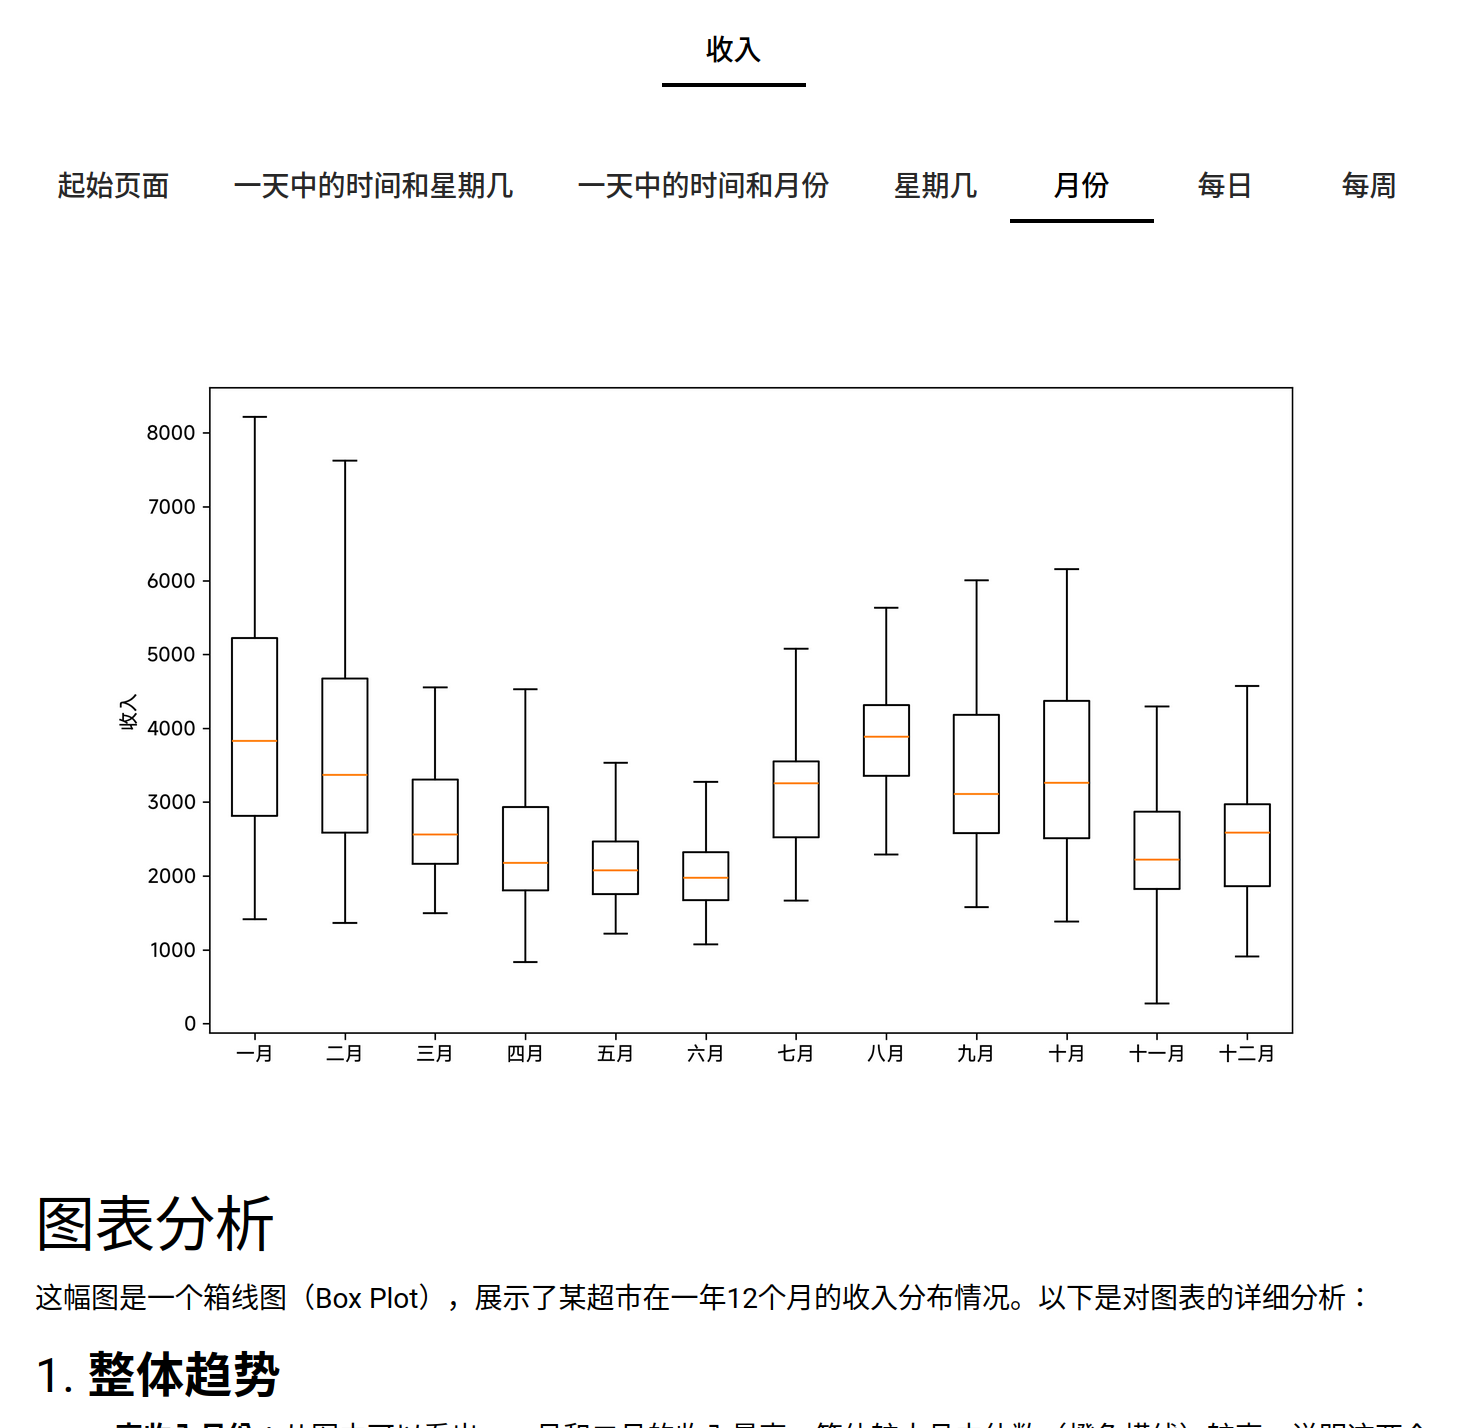
\includegraphics[width=0.5\textwidth]{./exp/aly-demo-3.png}
	\caption{(todo)}
	\label{fig:aly-demo-3}
\end{figure}

\begin{figure}[htbp]
	\centering
	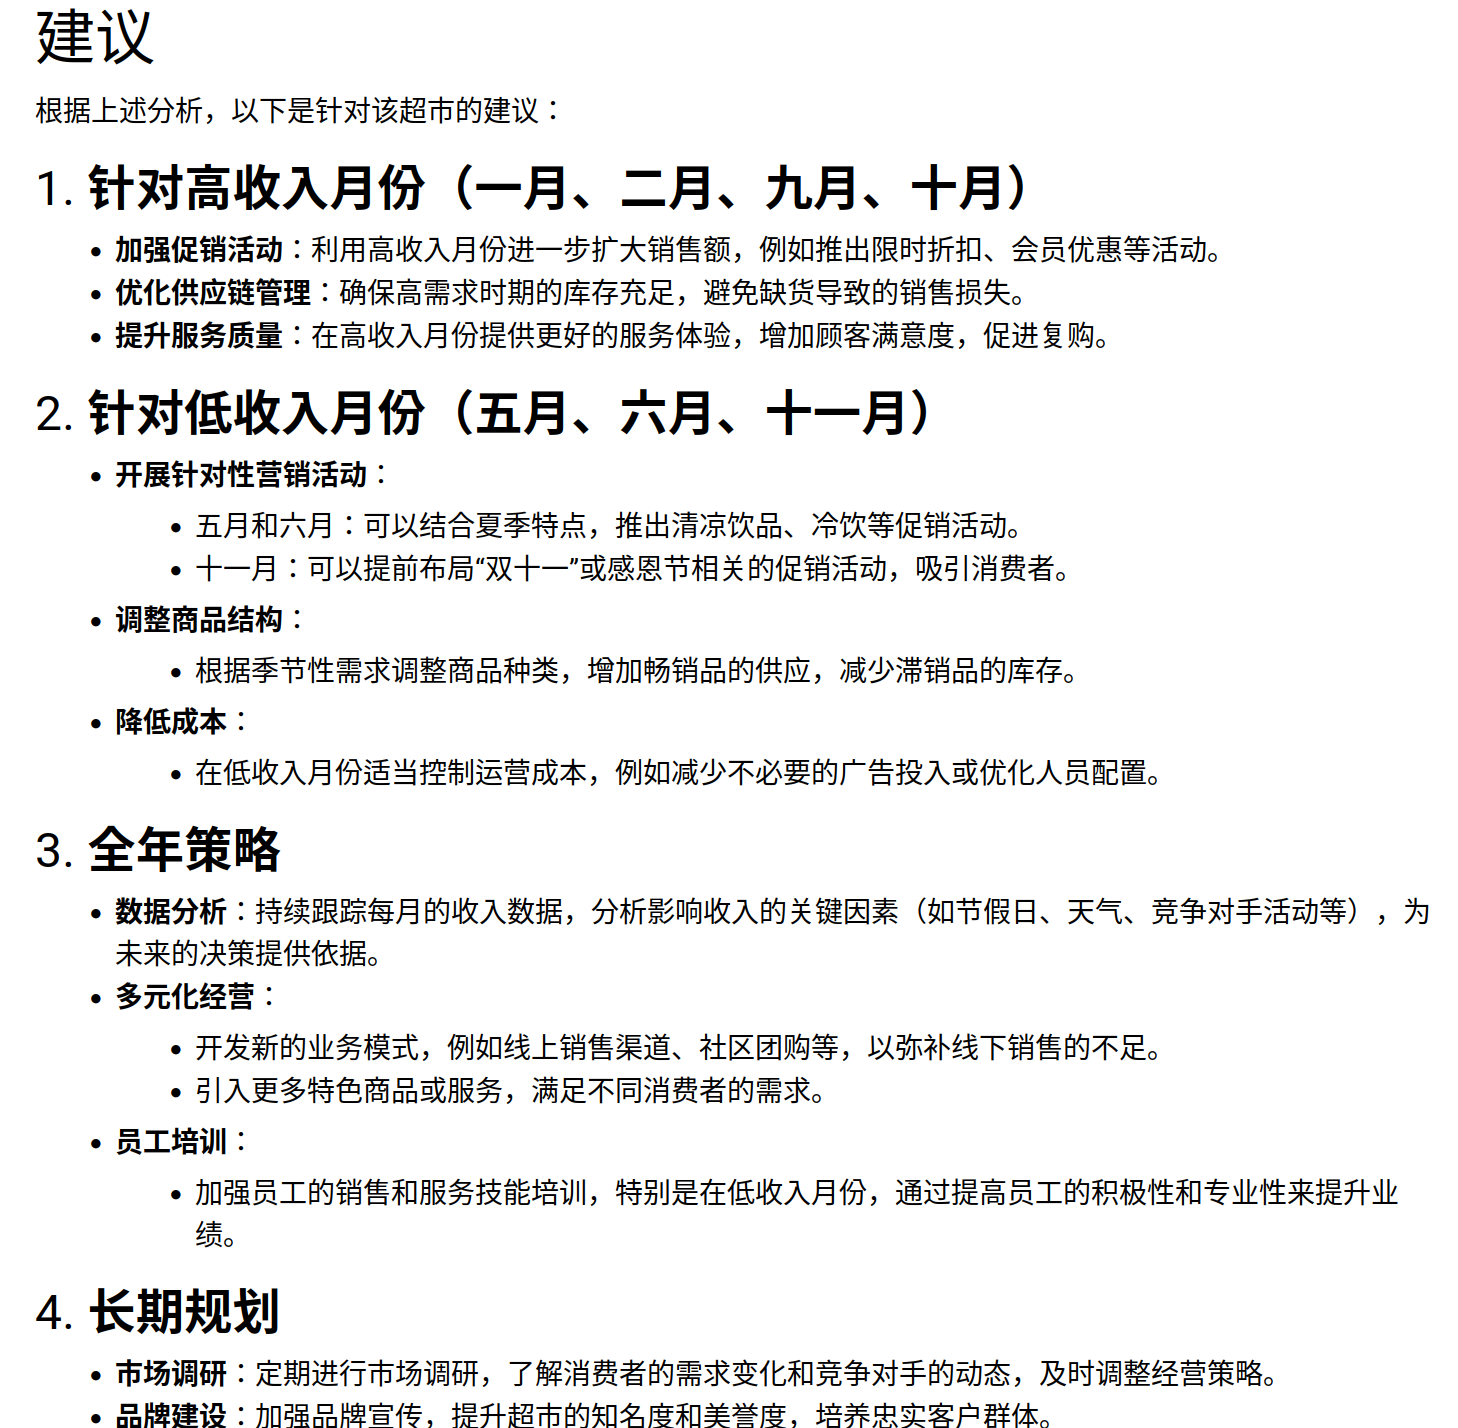
\includegraphics[width=0.5\textwidth]{./exp/aly-demo-4.png}
	\caption{(todo)}
	\label{fig:aly-demo-4}
\end{figure}

\begin{figure}[htbp]
	\centering
	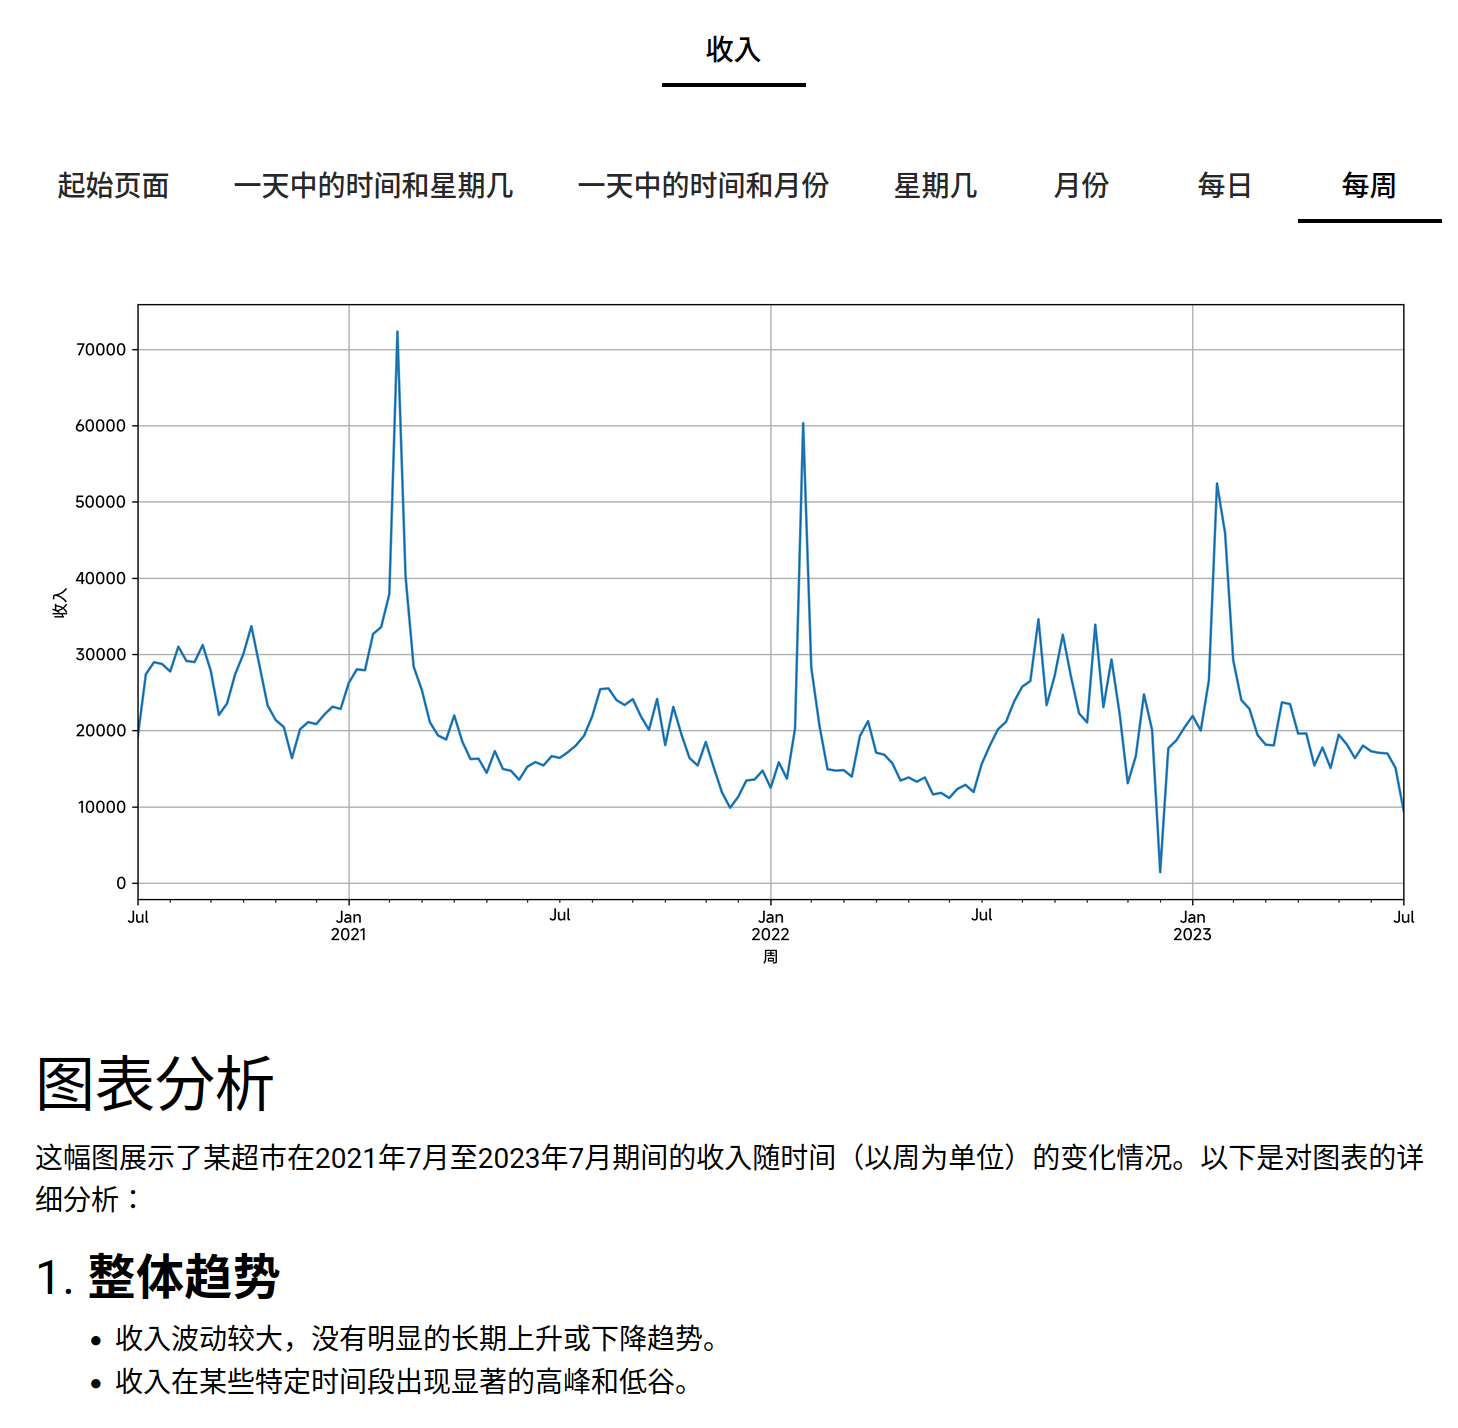
\includegraphics[width=0.5\textwidth]{./exp/aly-demo-5.png}
	\caption{(todo)}
	\label{fig:aly-demo-5}
\end{figure}

\subsubsection{ShopEyes Owner}

\begin{figure}[htbp]
    \centering
    \subfloat{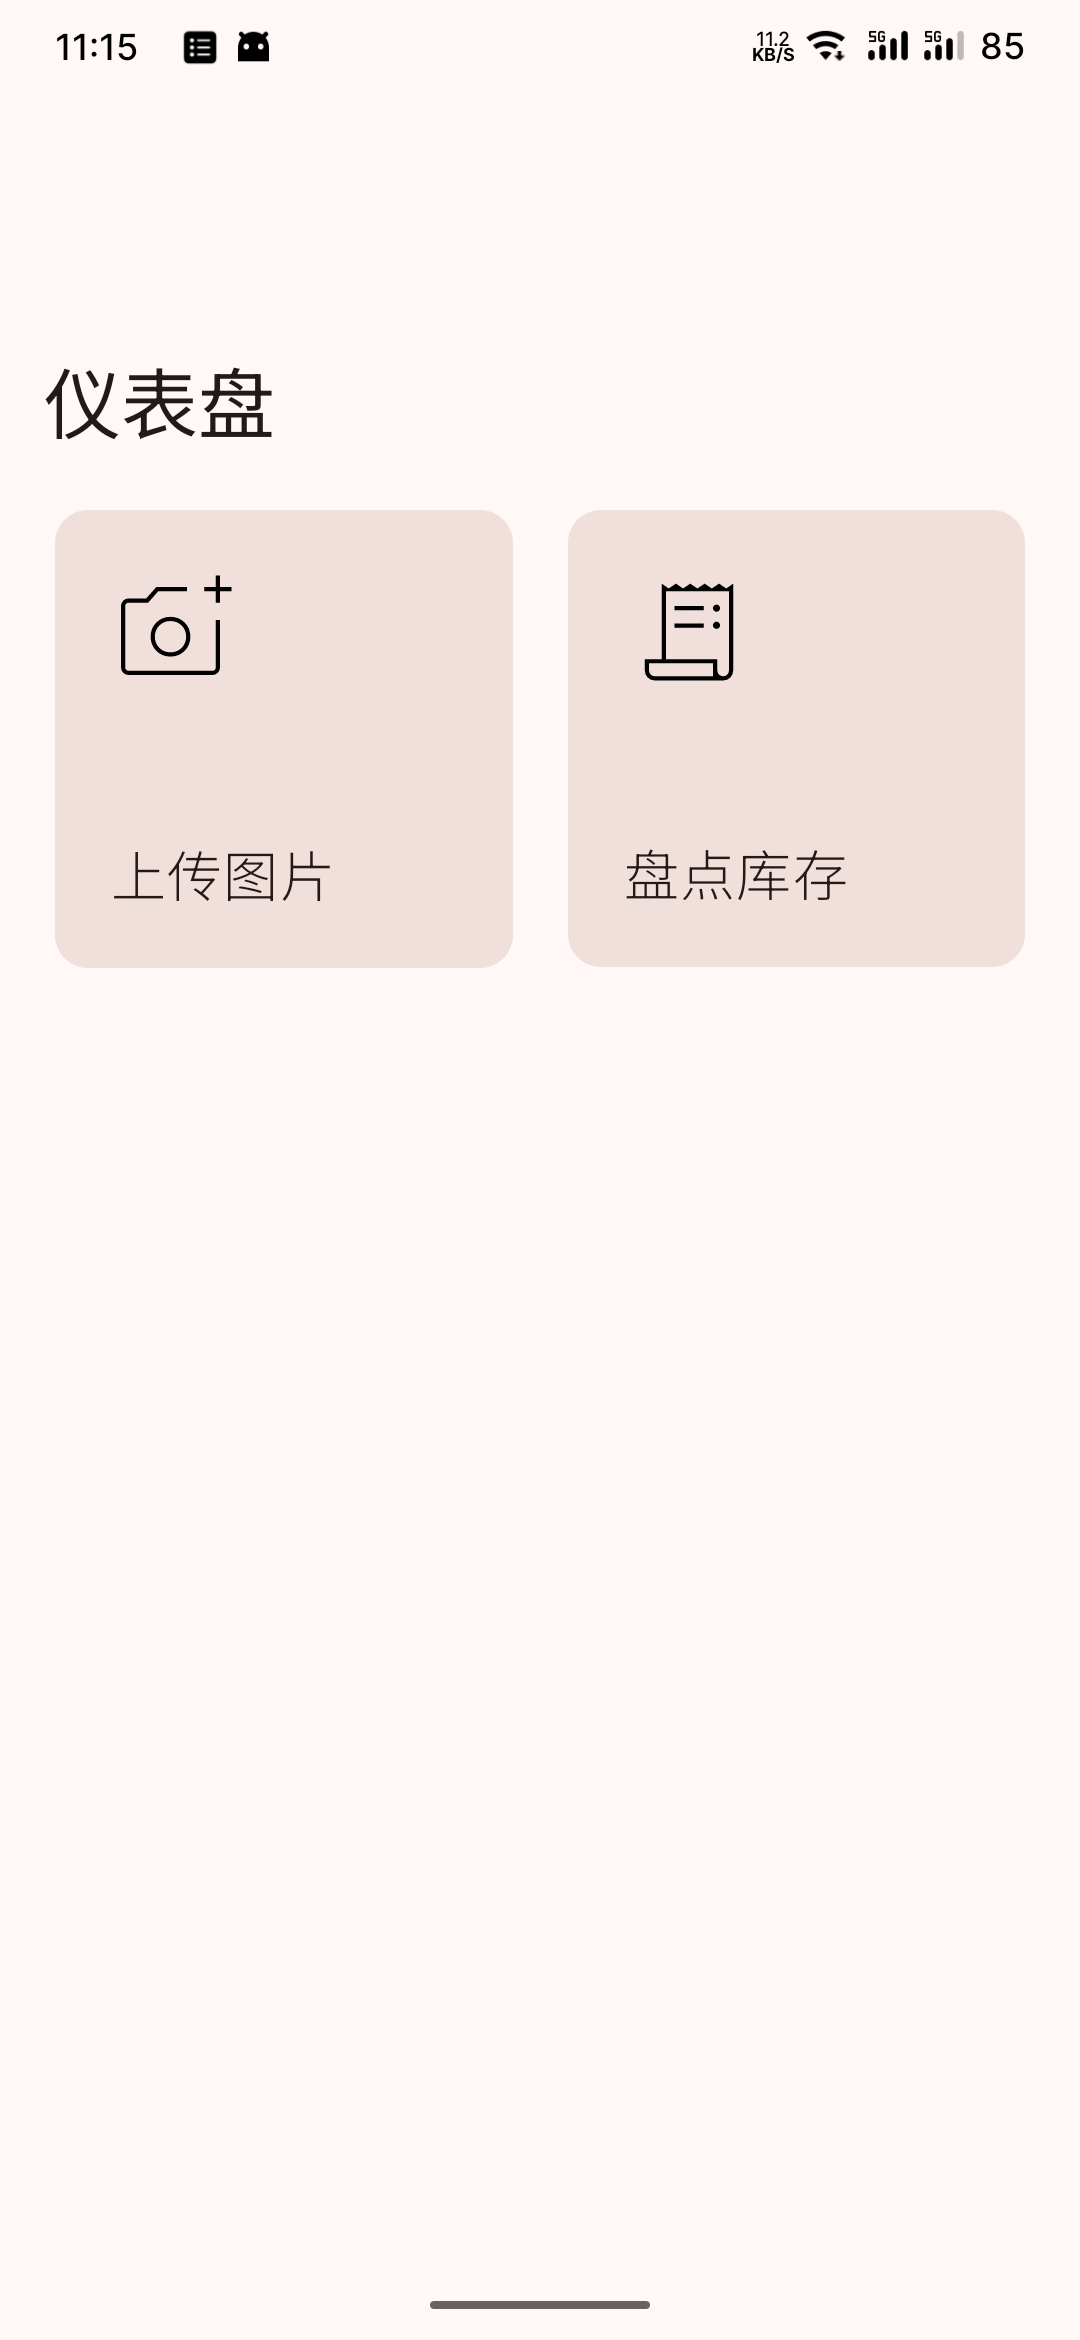
\includegraphics[width=0.2475\textwidth]{./exp/seo.png}}
    \hfill
    \subfloat{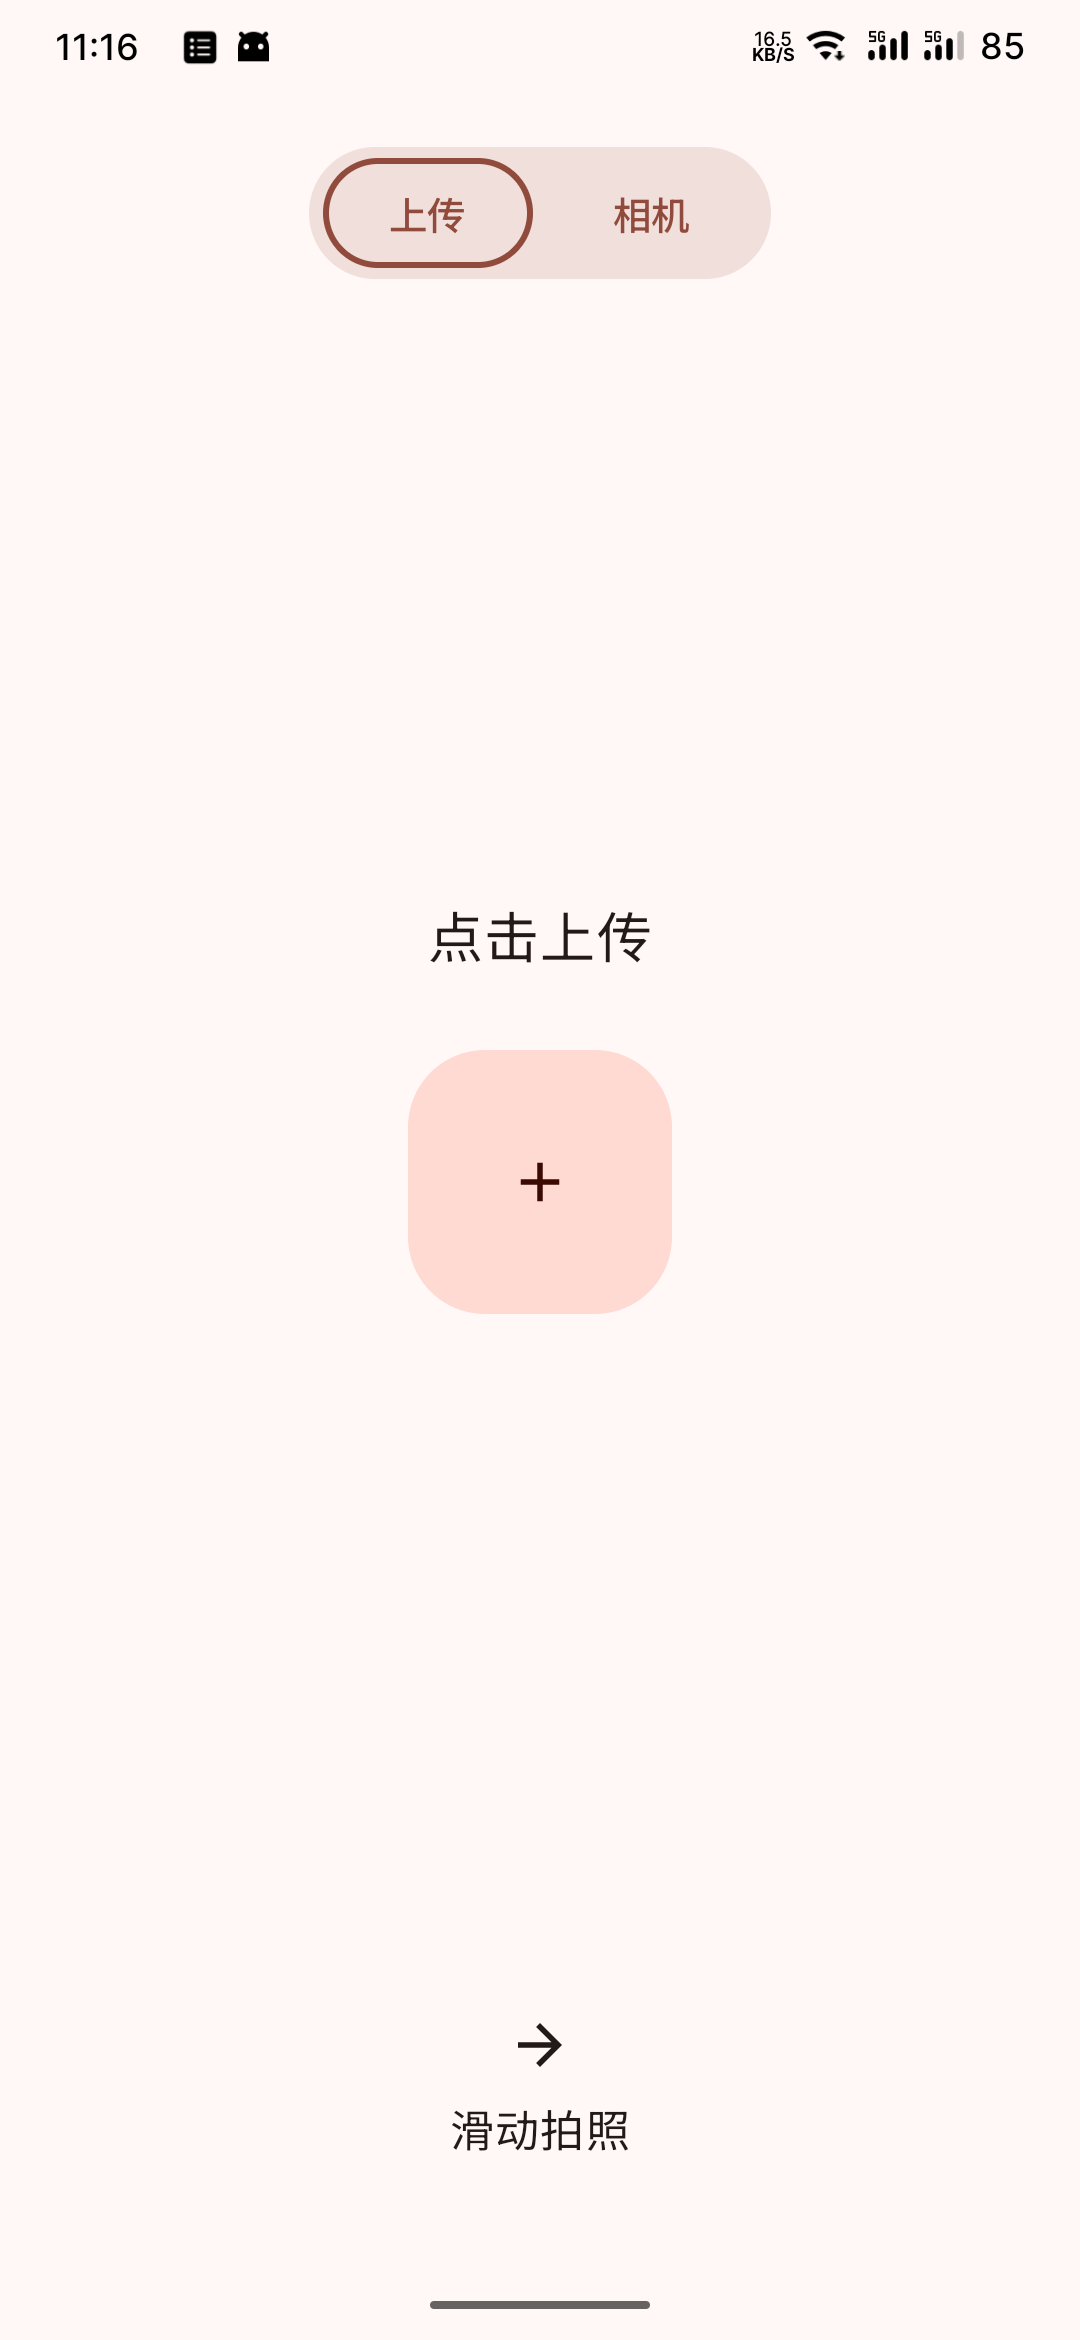
\includegraphics[width=0.2475\textwidth]{./exp/seo-local.png}}
    \hfill
    \subfloat{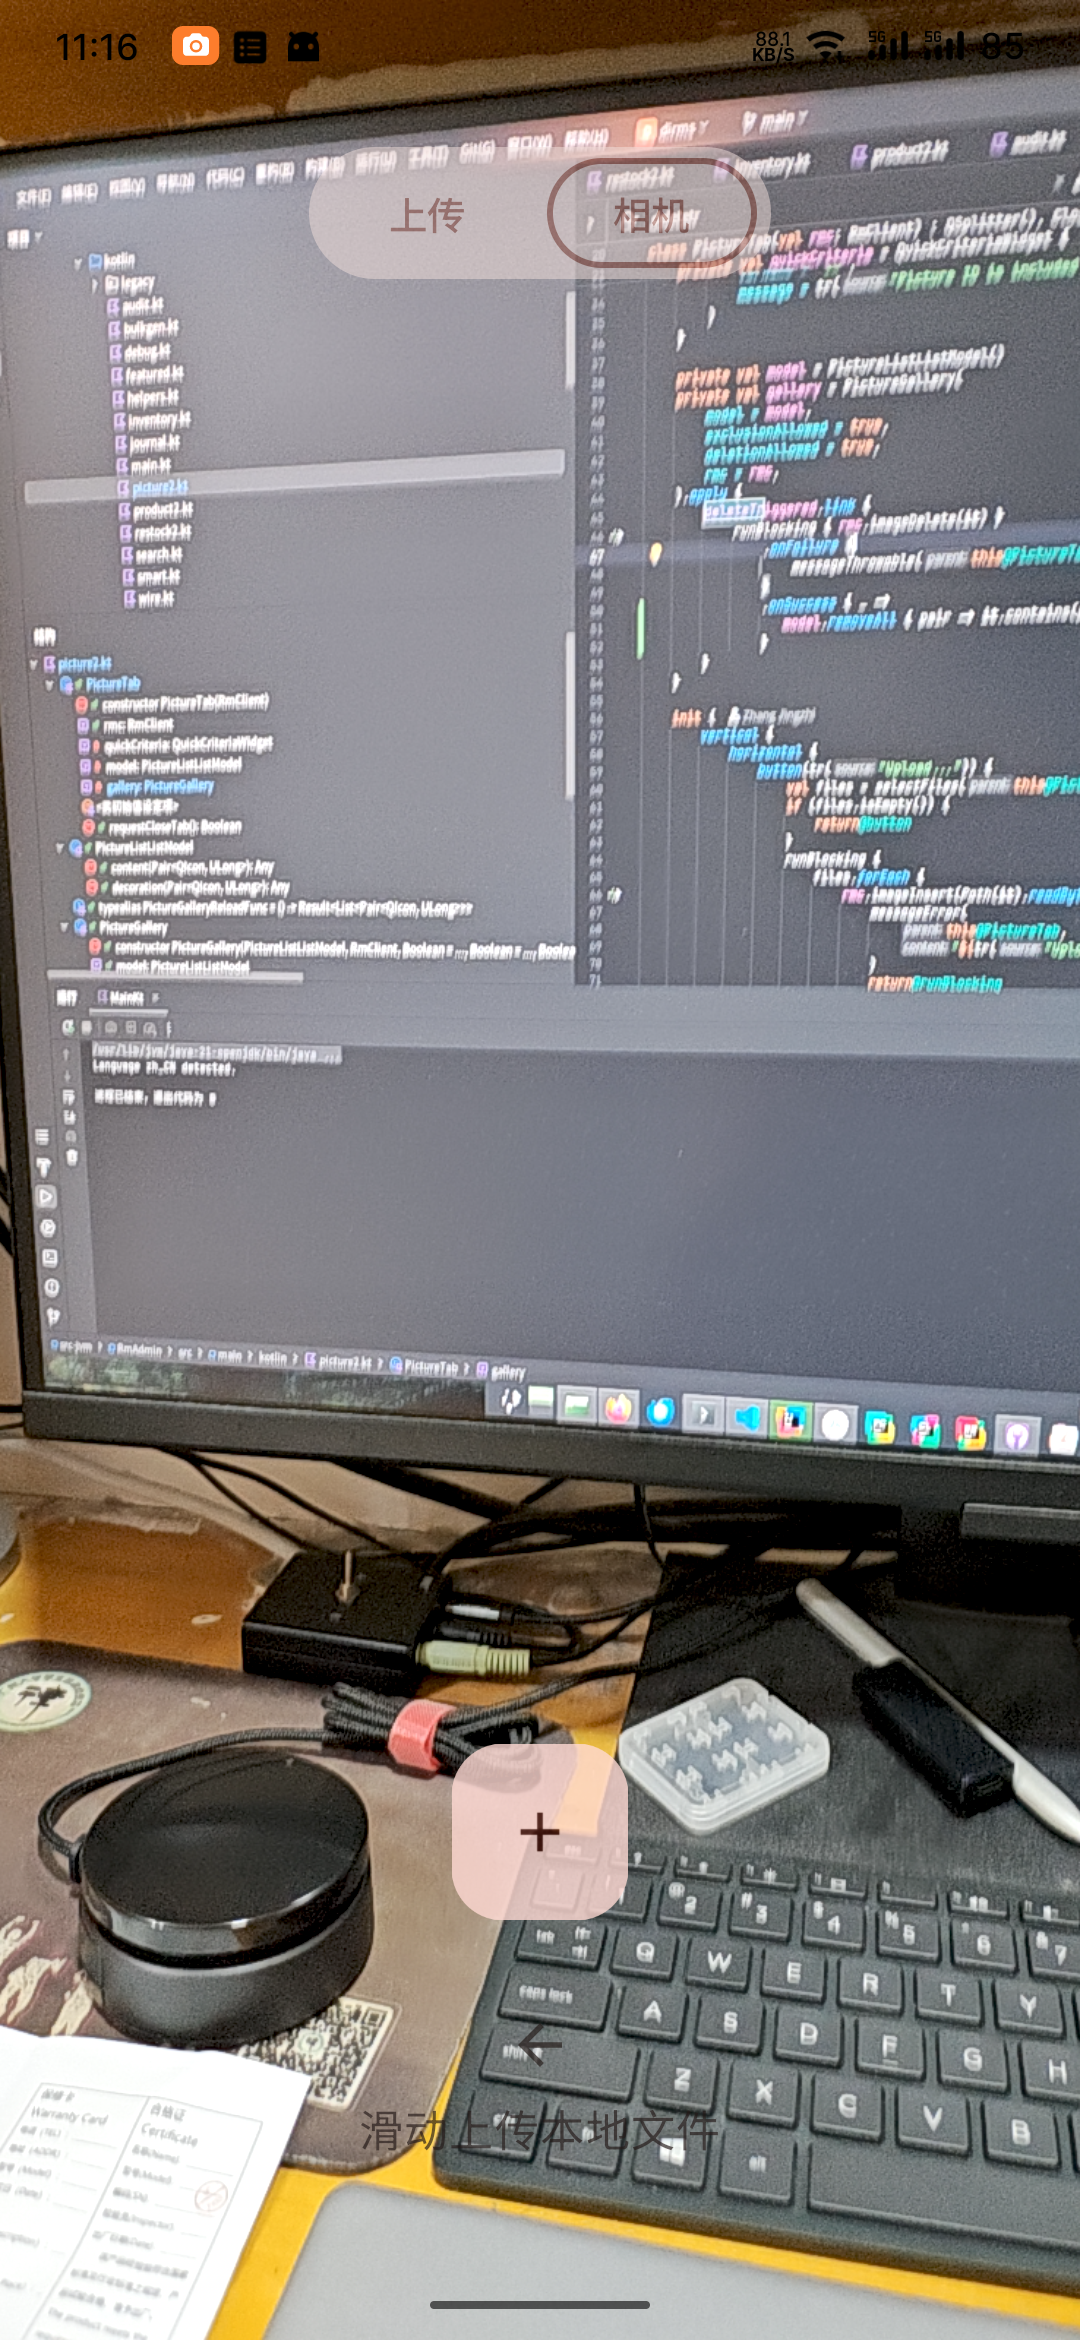
\includegraphics[width=0.2475\textwidth]{./exp/seo-camera.png}}
    \hfill
    \subfloat{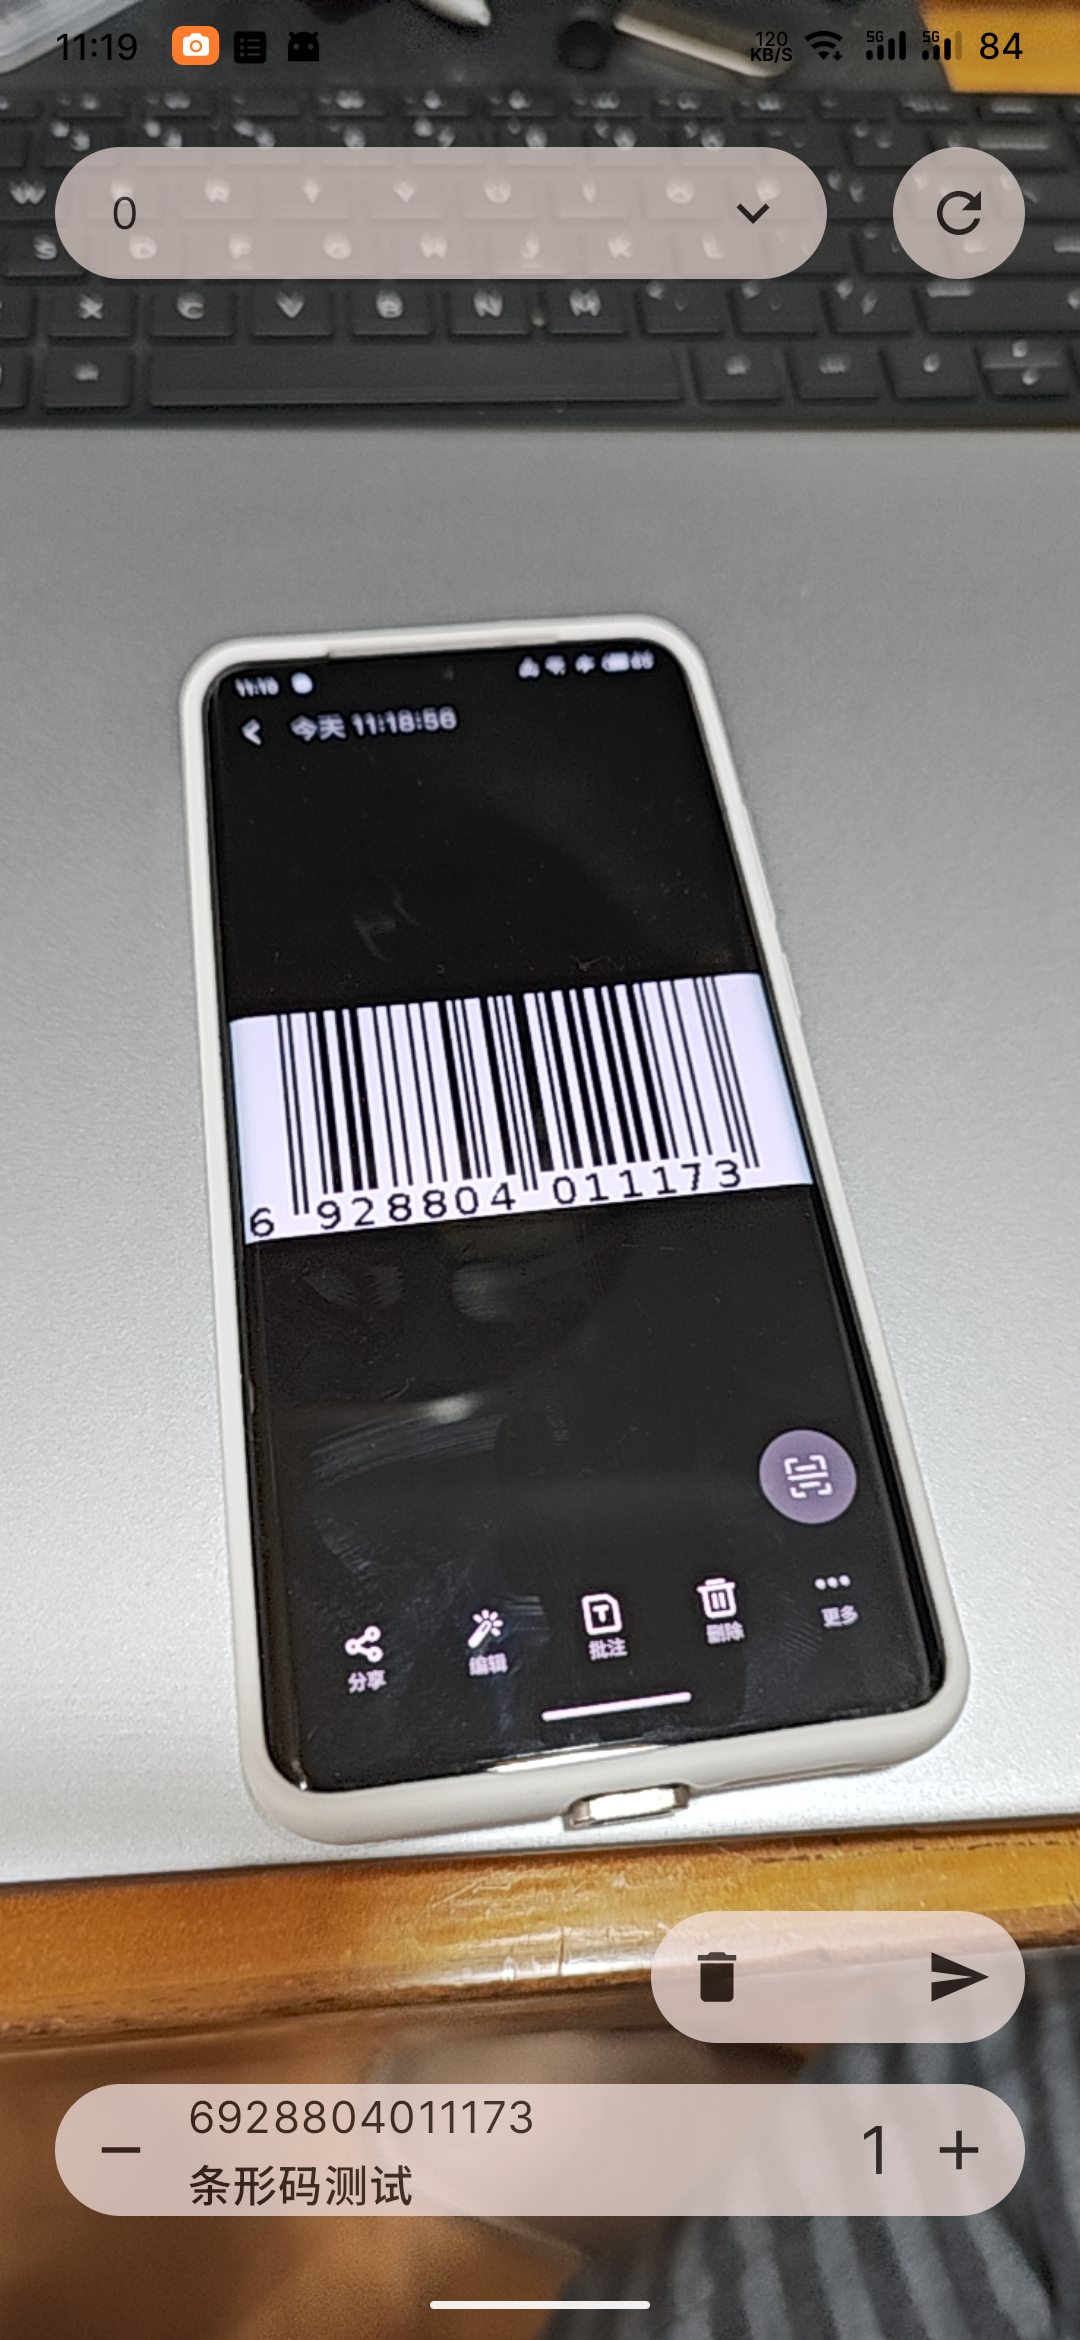
\includegraphics[width=0.2475\textwidth]{./exp/seo-audit.png}}
	\caption{(todo)}
	\label{fig:seo}
\end{figure}

\subsubsection{EasyDataset}

\begin{figure}[htbp]
    \subfloat{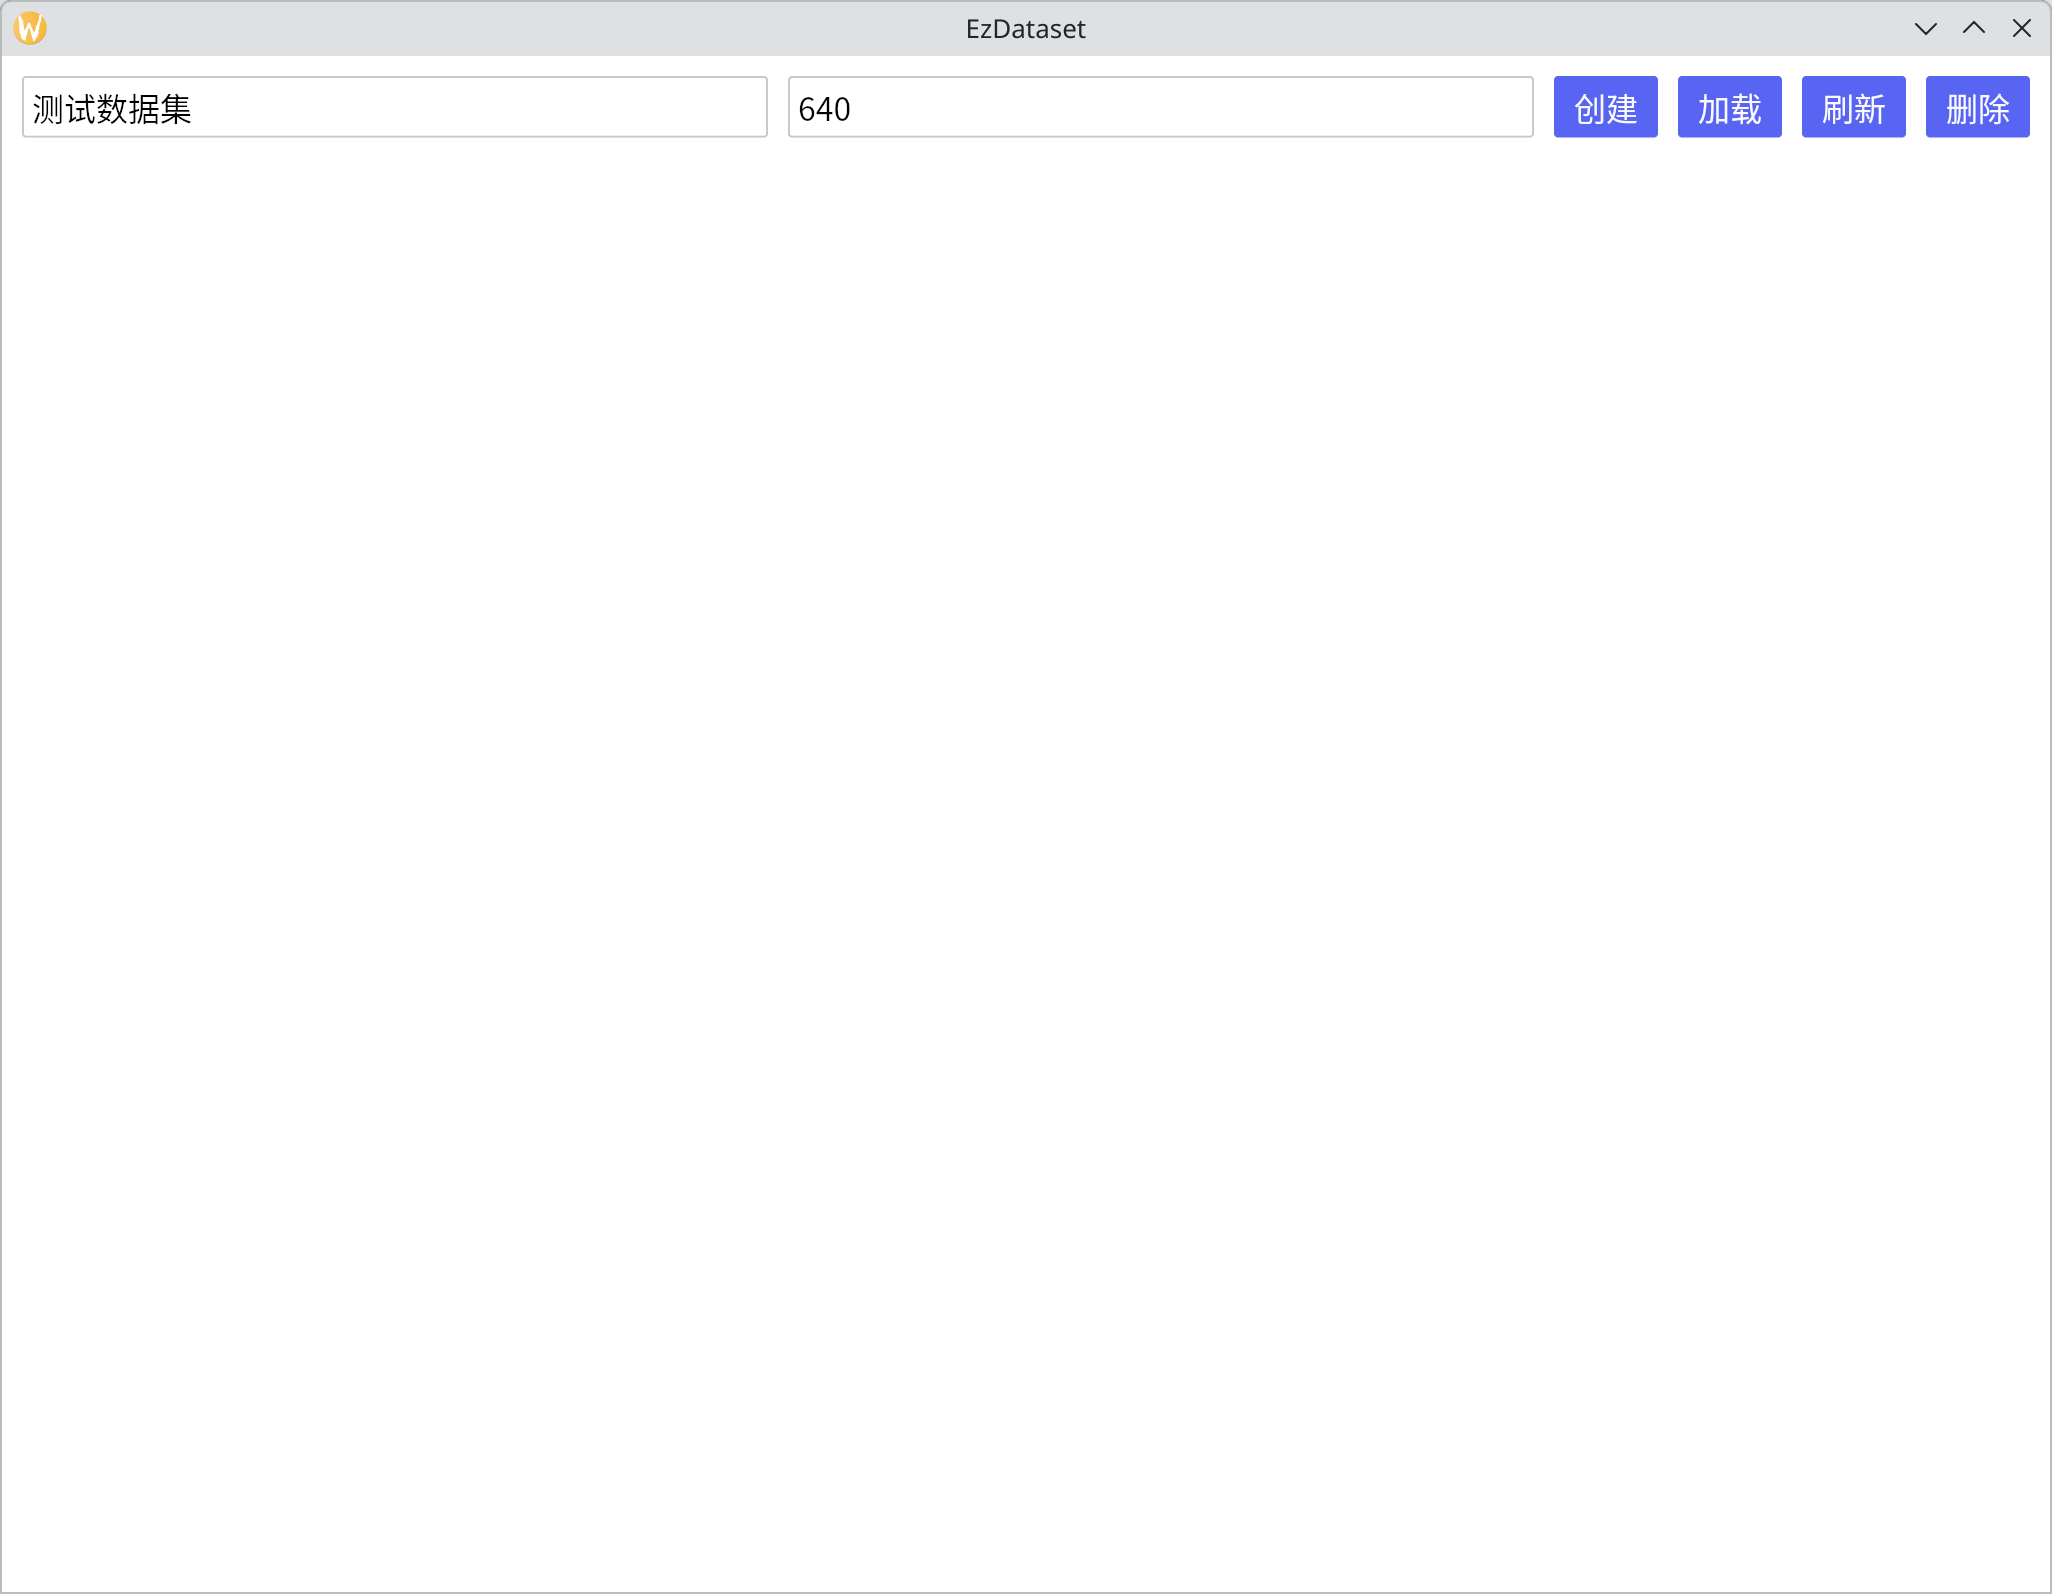
\includegraphics[width=0.45\textwidth]{./exp/ed-nd-1.png}}
    \hfill
    \subfloat{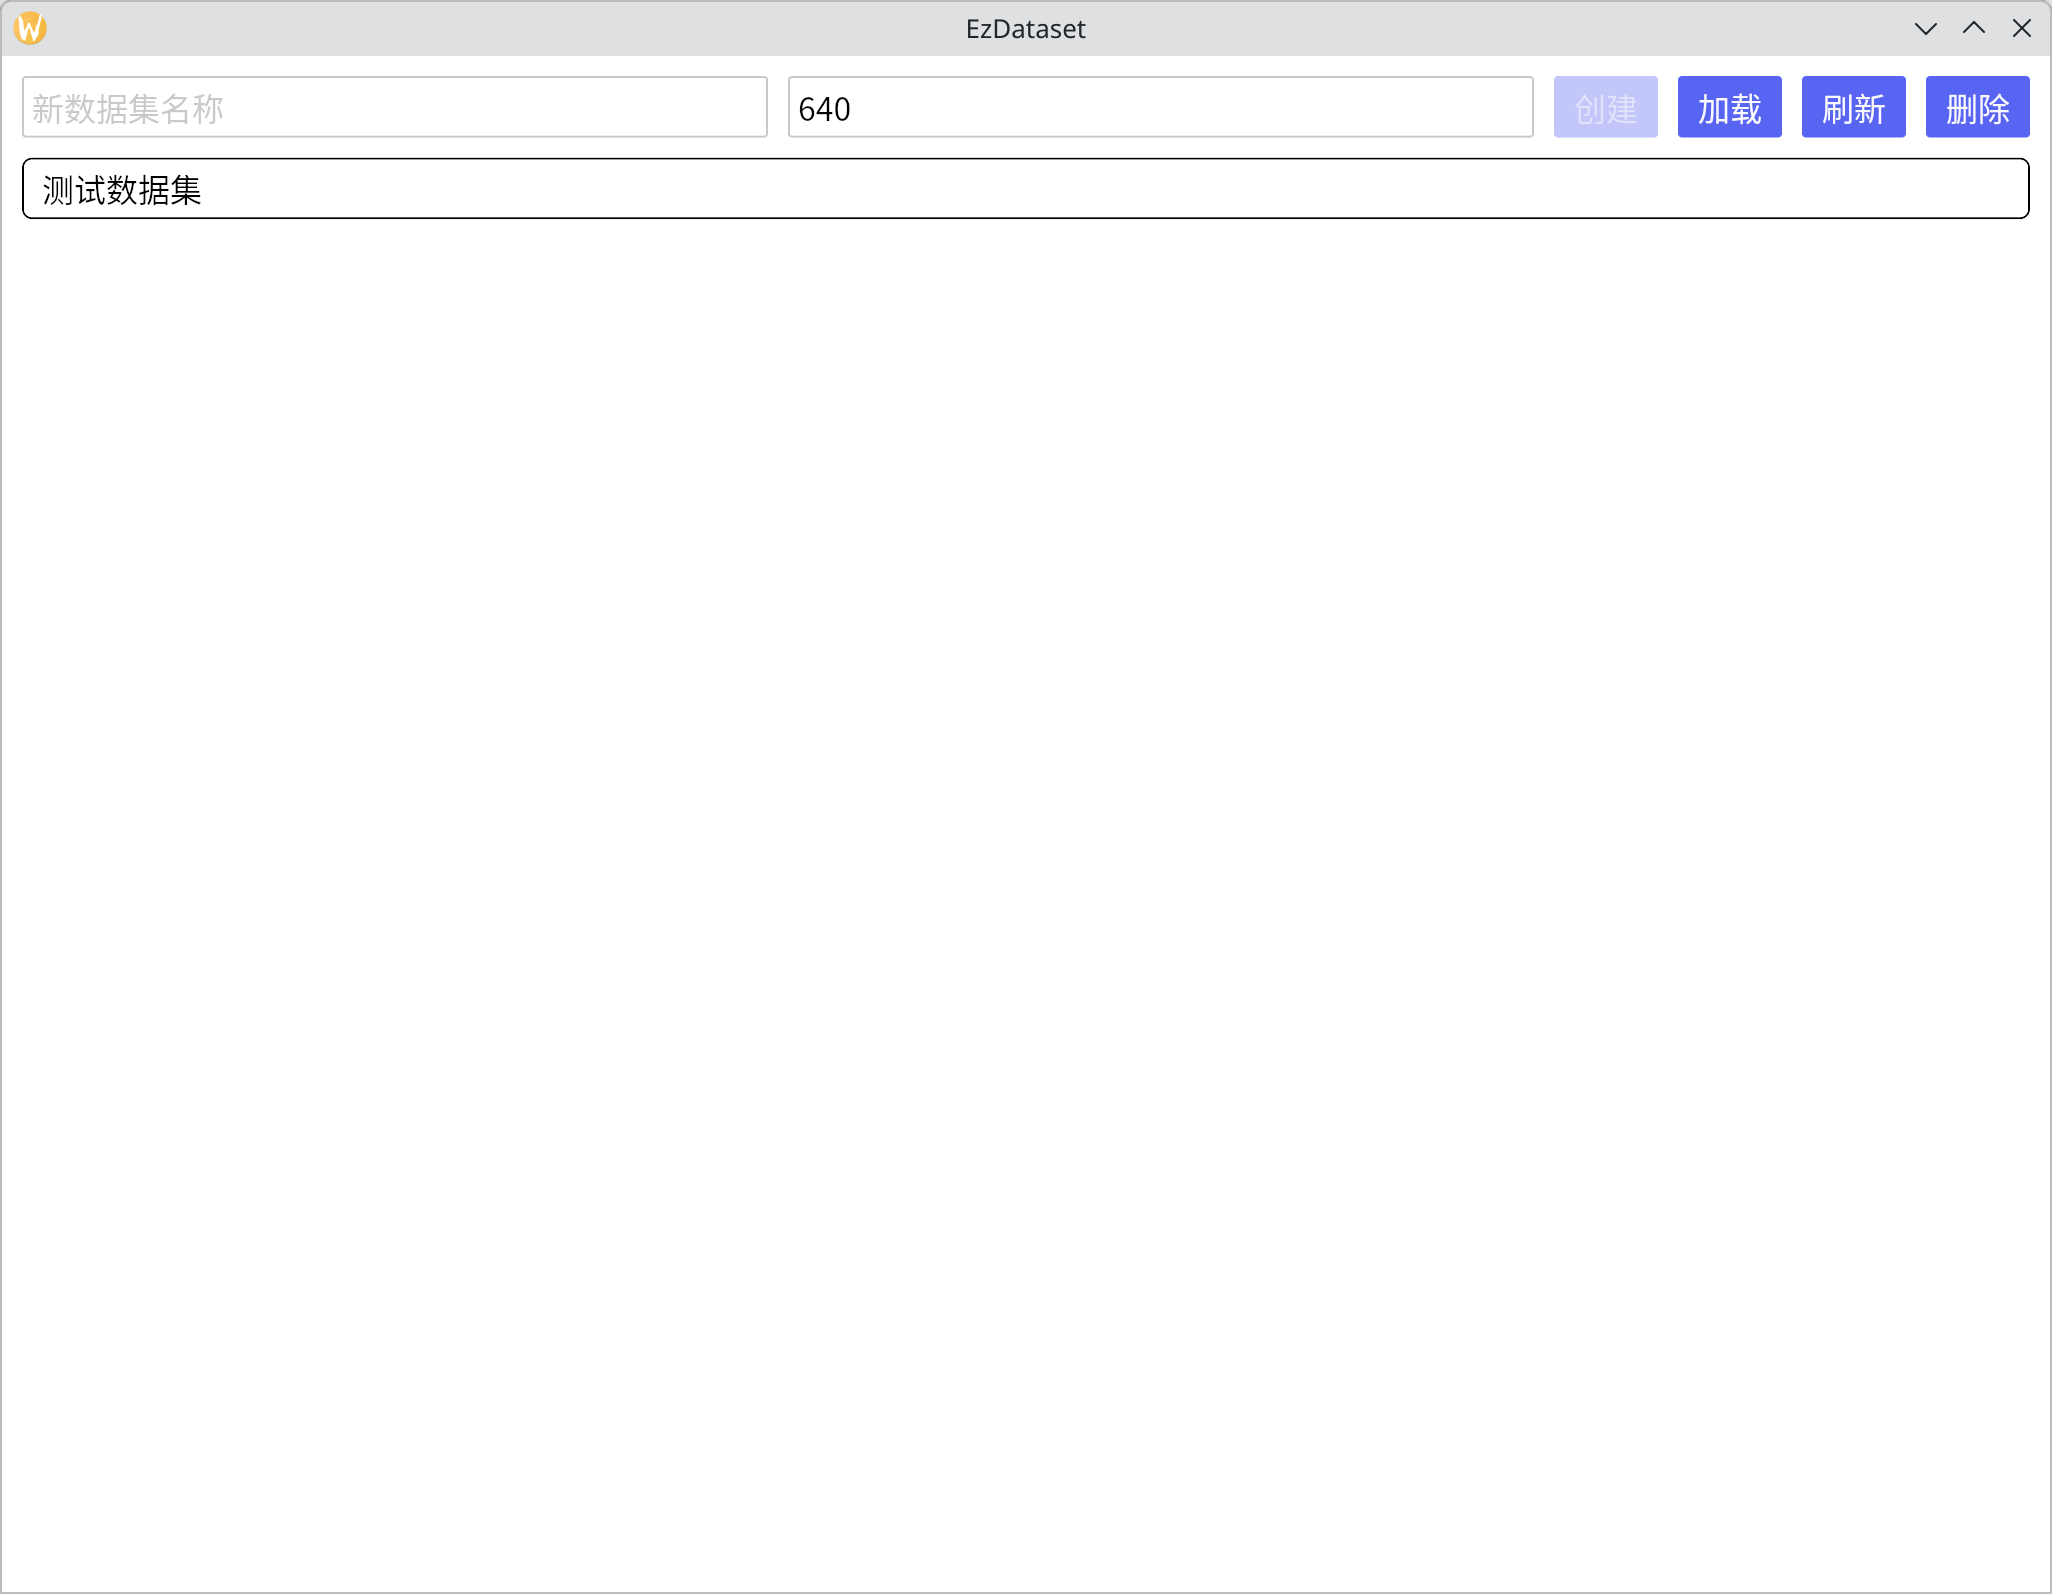
\includegraphics[width=0.45\textwidth]{./exp/ed-nd-2.png}}
	\caption{(todo)}
	\label{fig:ed-nd}
\end{figure}

\begin{figure}[htbp]
    \subfloat{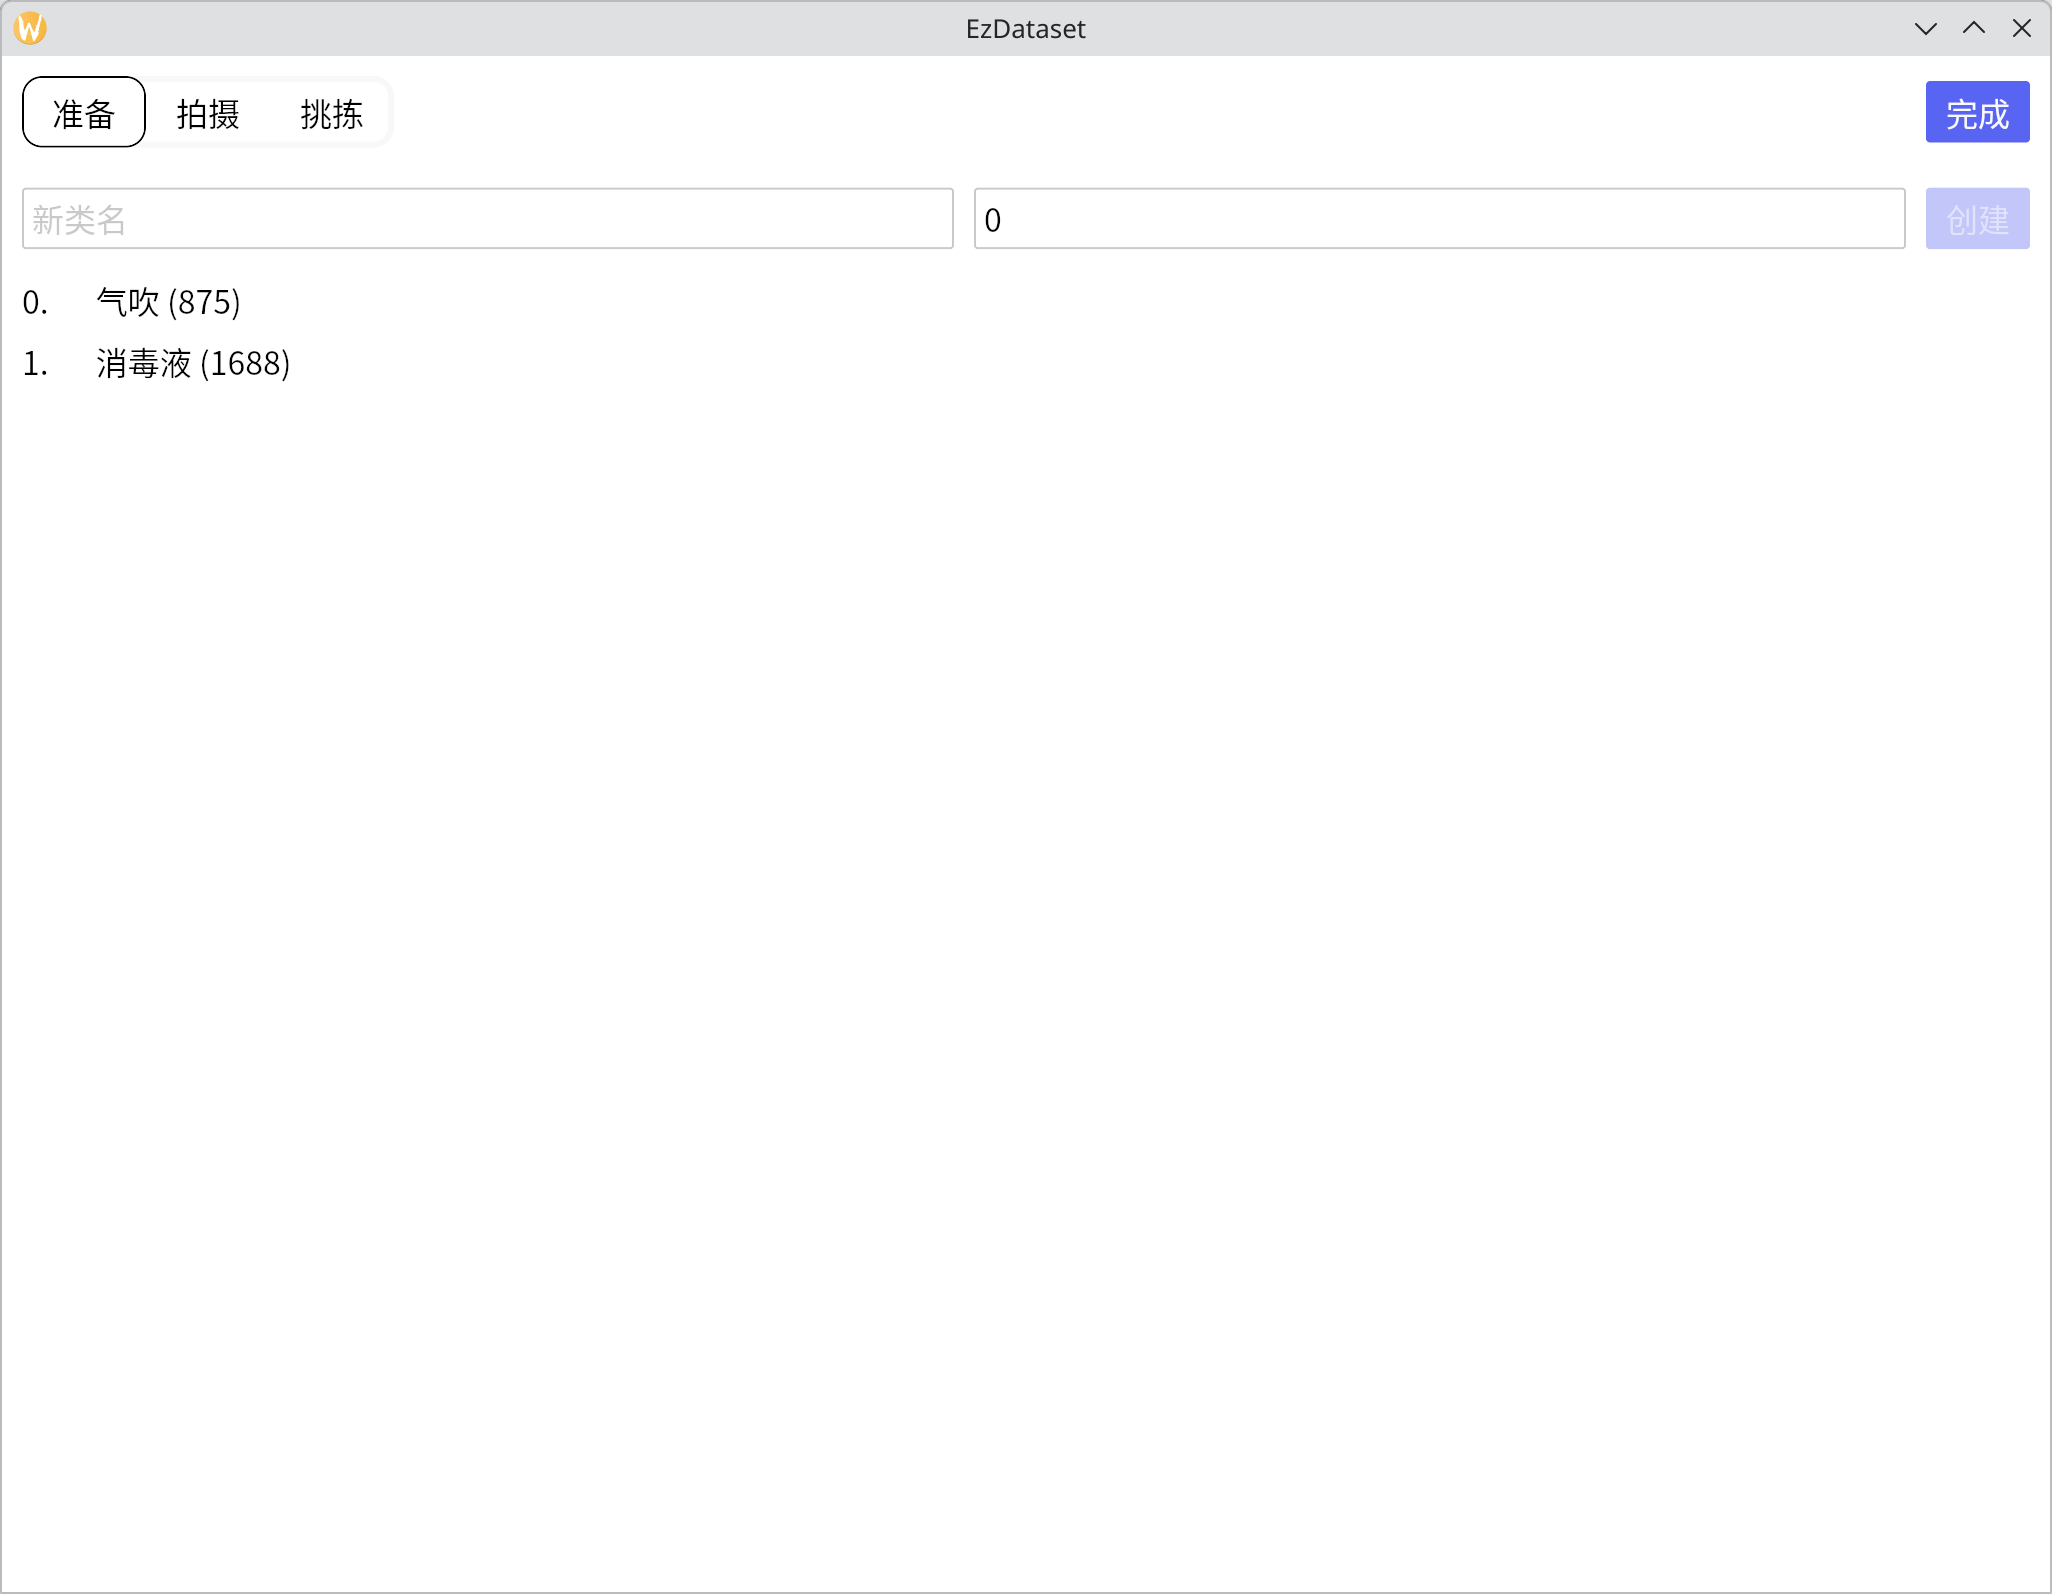
\includegraphics[width=0.45\textwidth]{./exp/ed-nc.png}}
    \hfill
    \subfloat{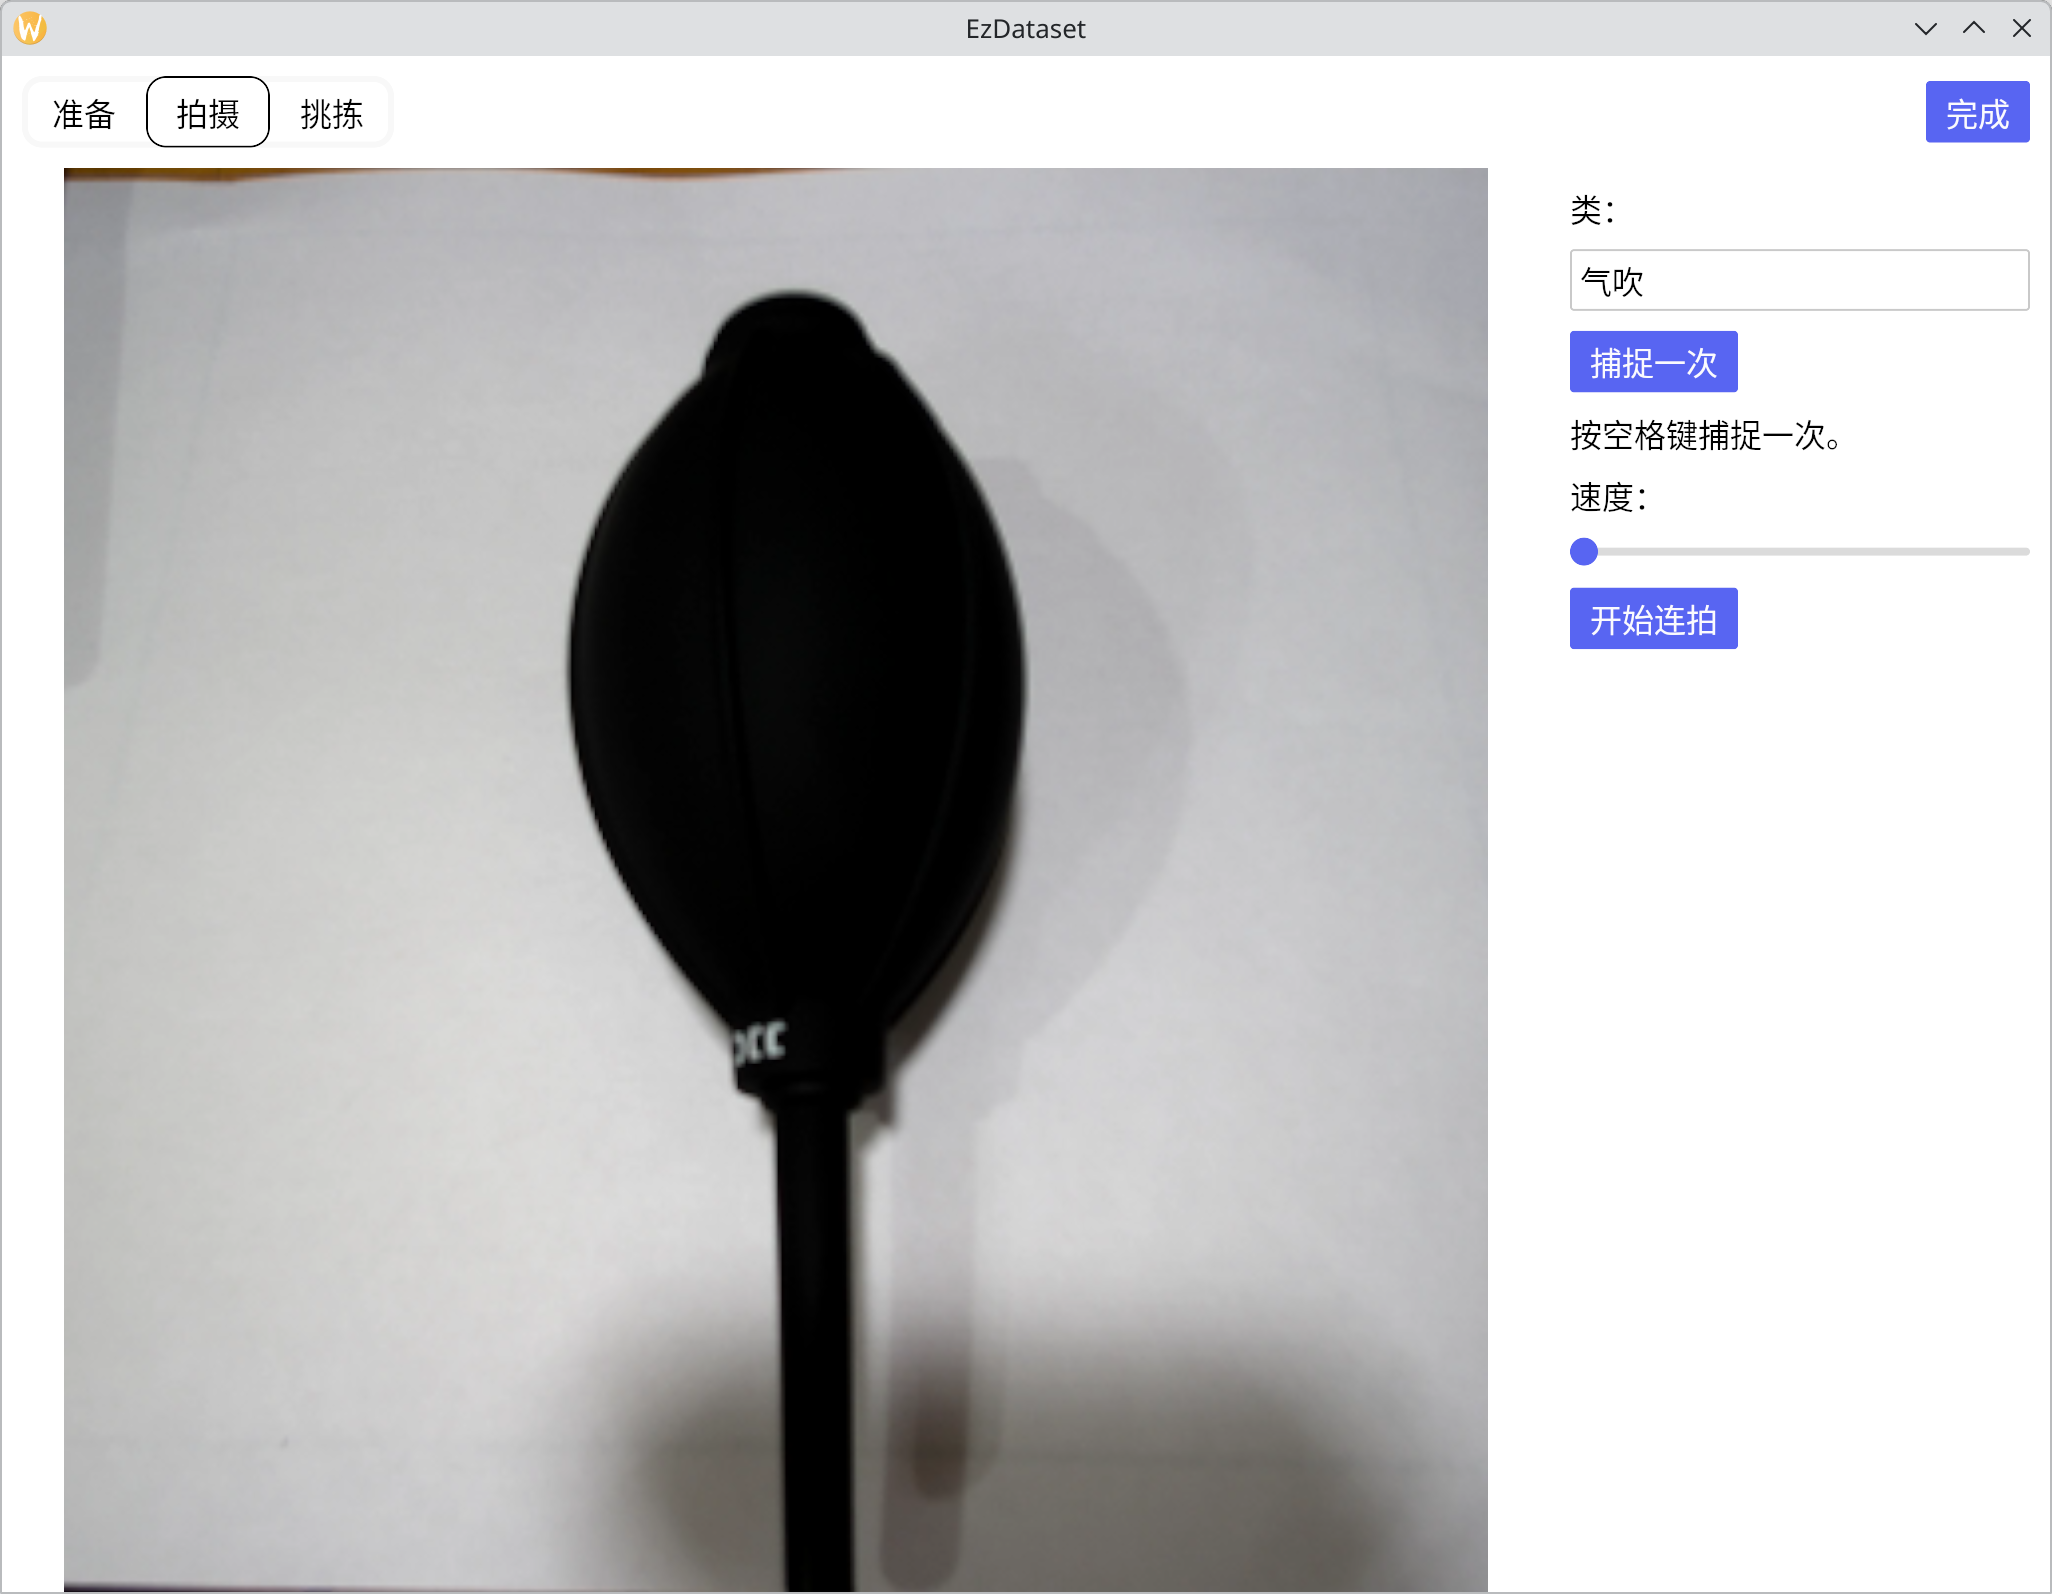
\includegraphics[width=0.45\textwidth]{./exp/ed-shot.png}}
    \hfill
    \subfloat{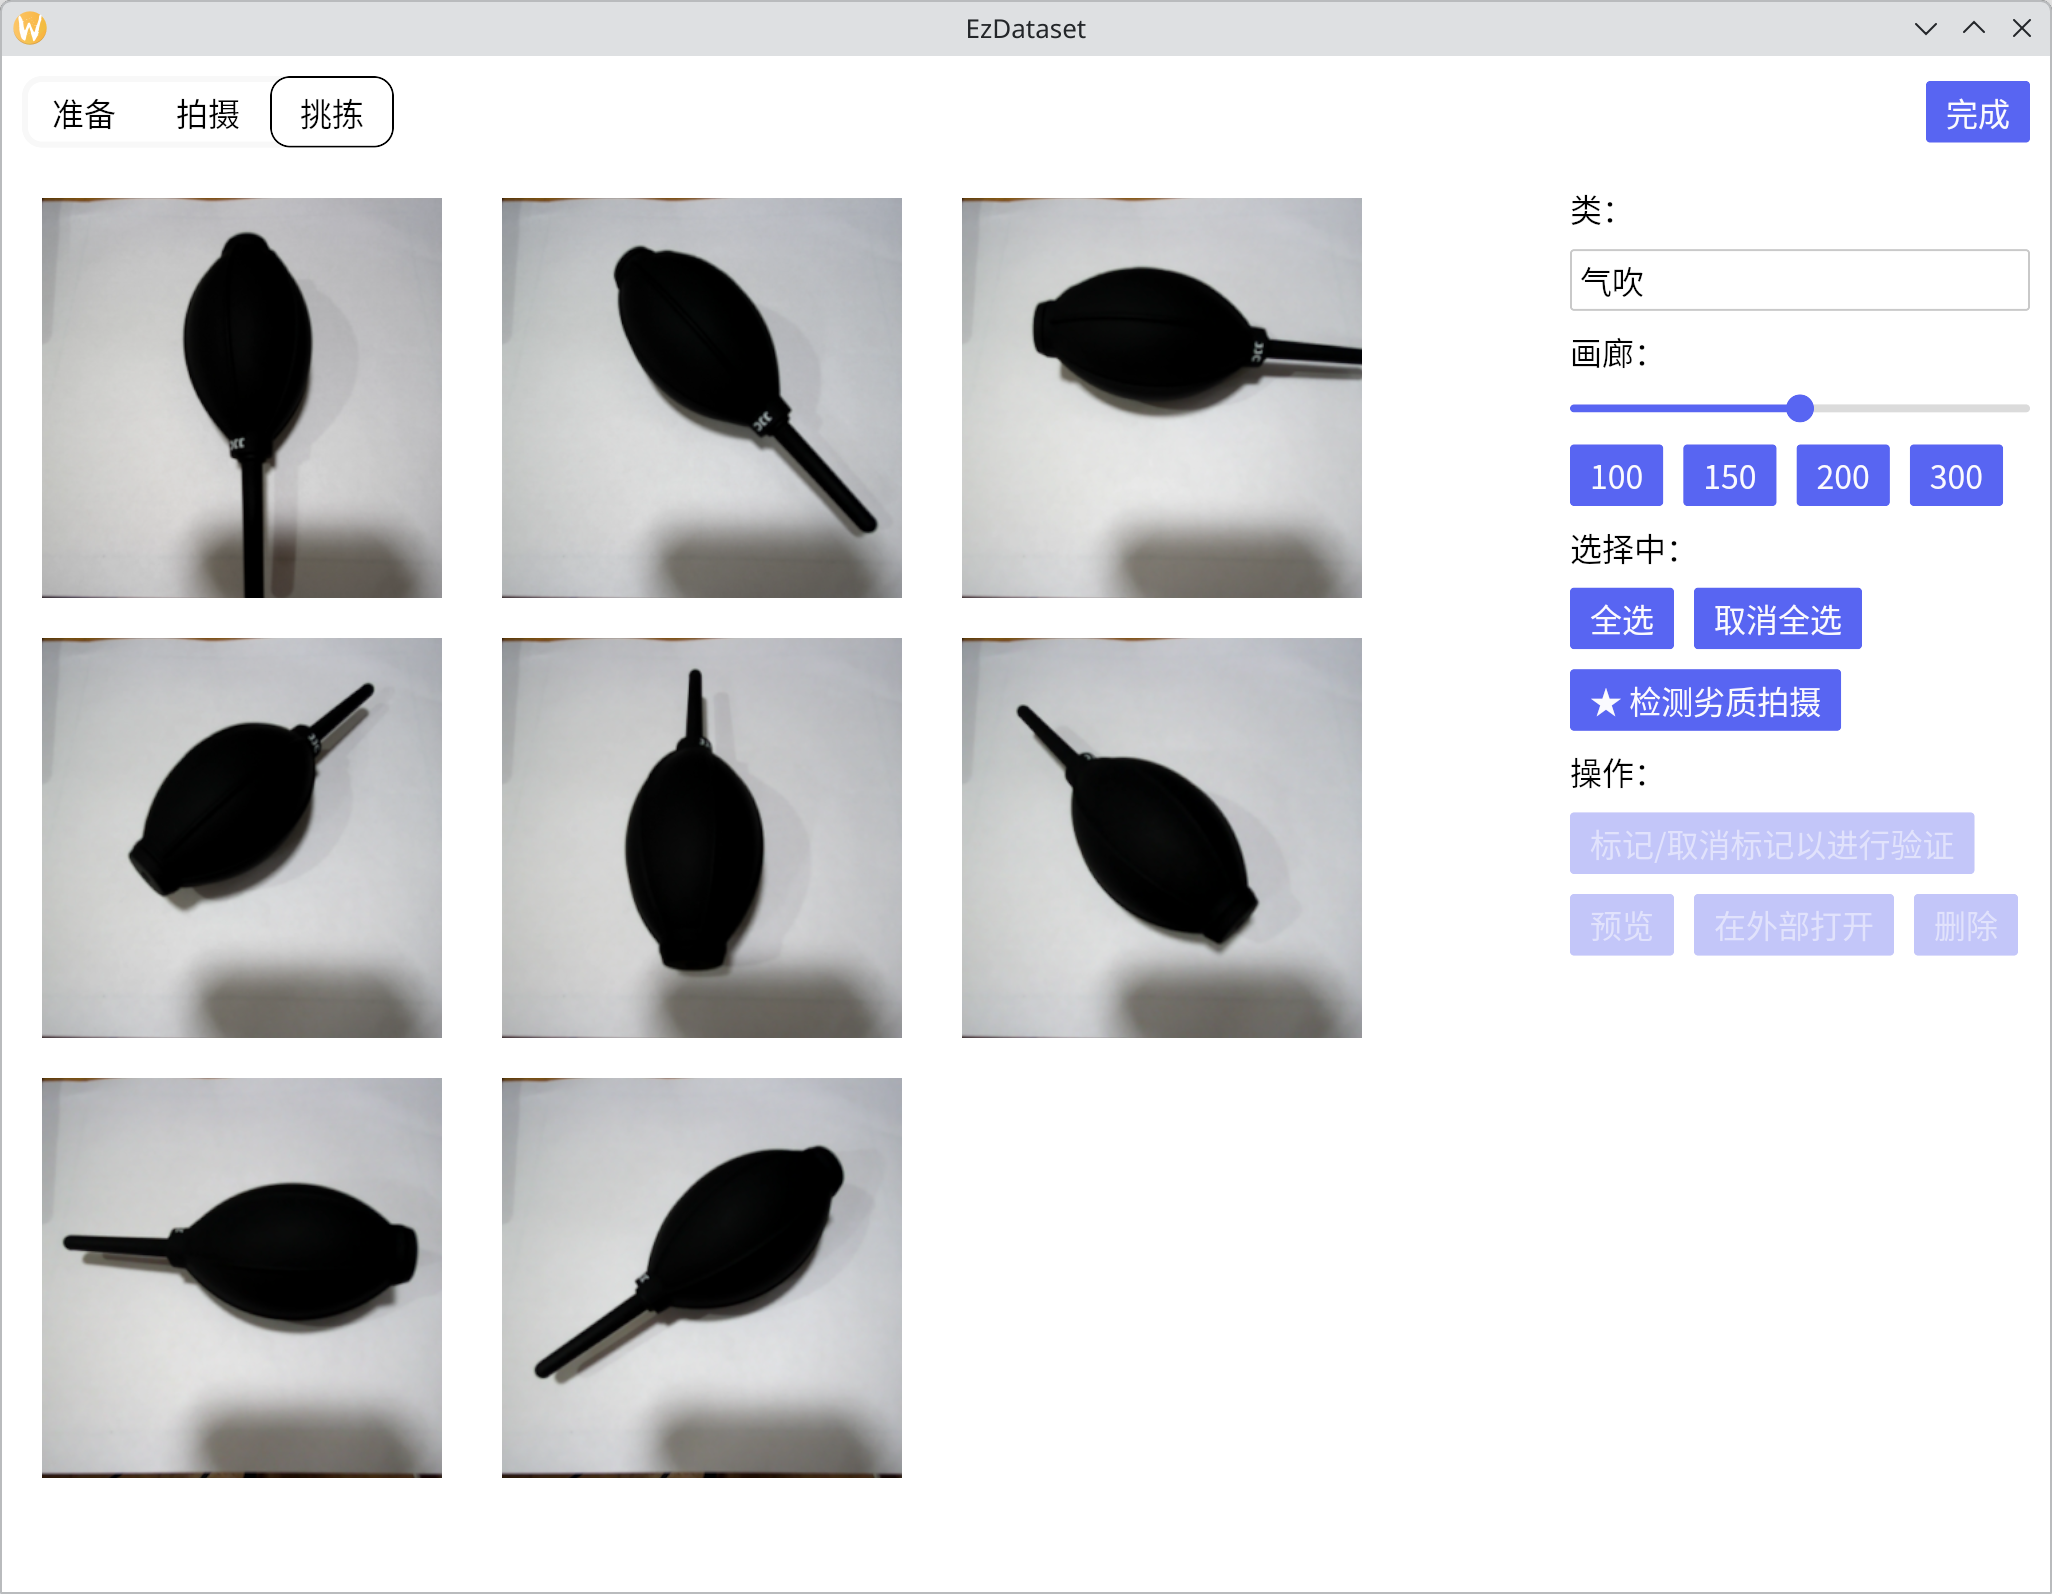
\includegraphics[width=0.45\textwidth]{./exp/ed-view.png}}
	\caption{(todo)}
	\label{fig:ed-edit}
\end{figure}

\subsection{顾客端}

\subsubsection{ShopEyes Guest}

\begin{figure}[htbp]
    \subfloat{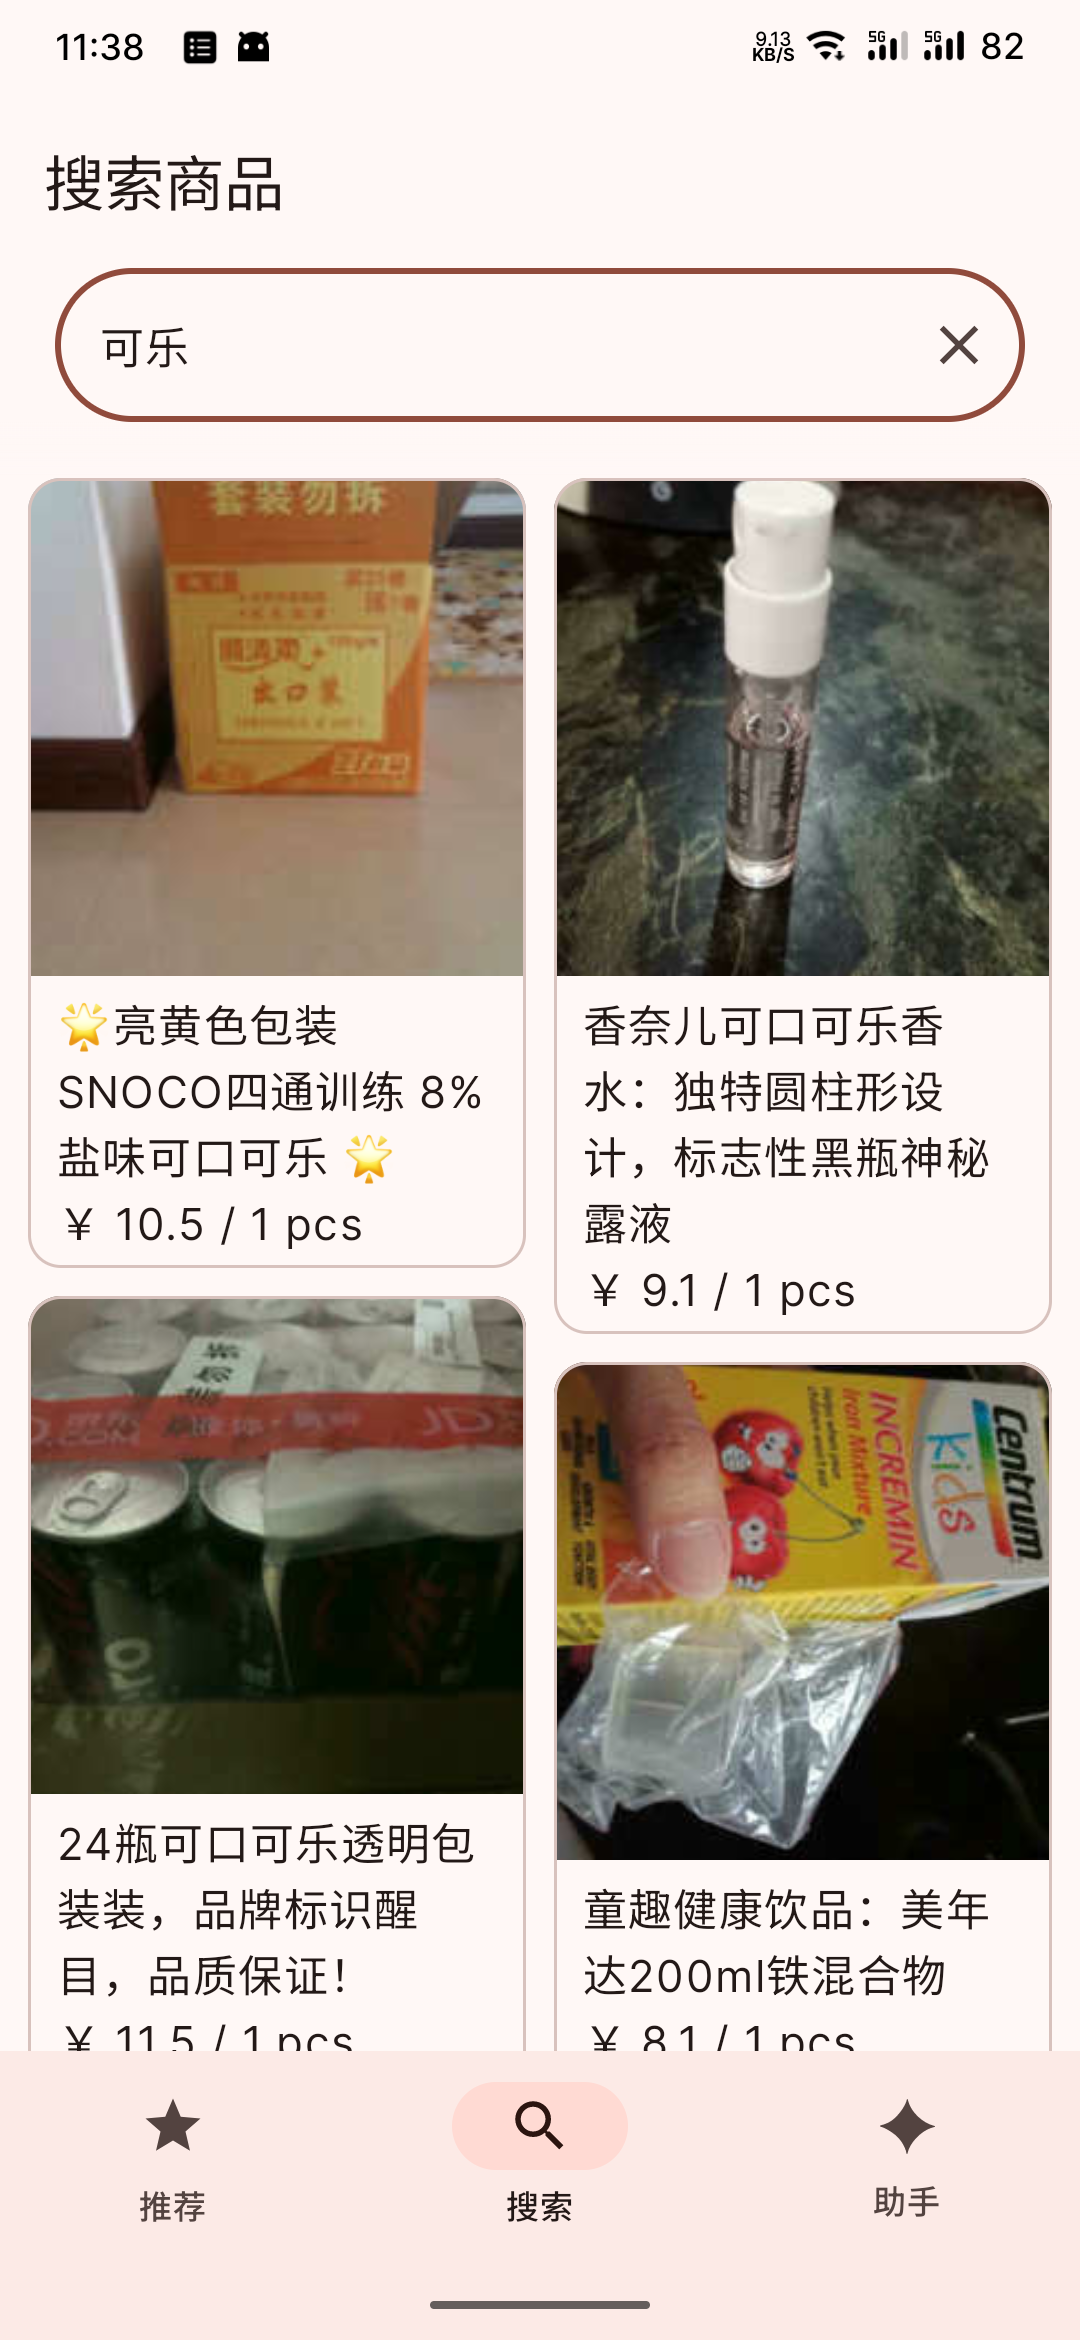
\includegraphics[width=0.3\textwidth]{./exp/seg-tx.png}}
    \hfill
    \subfloat{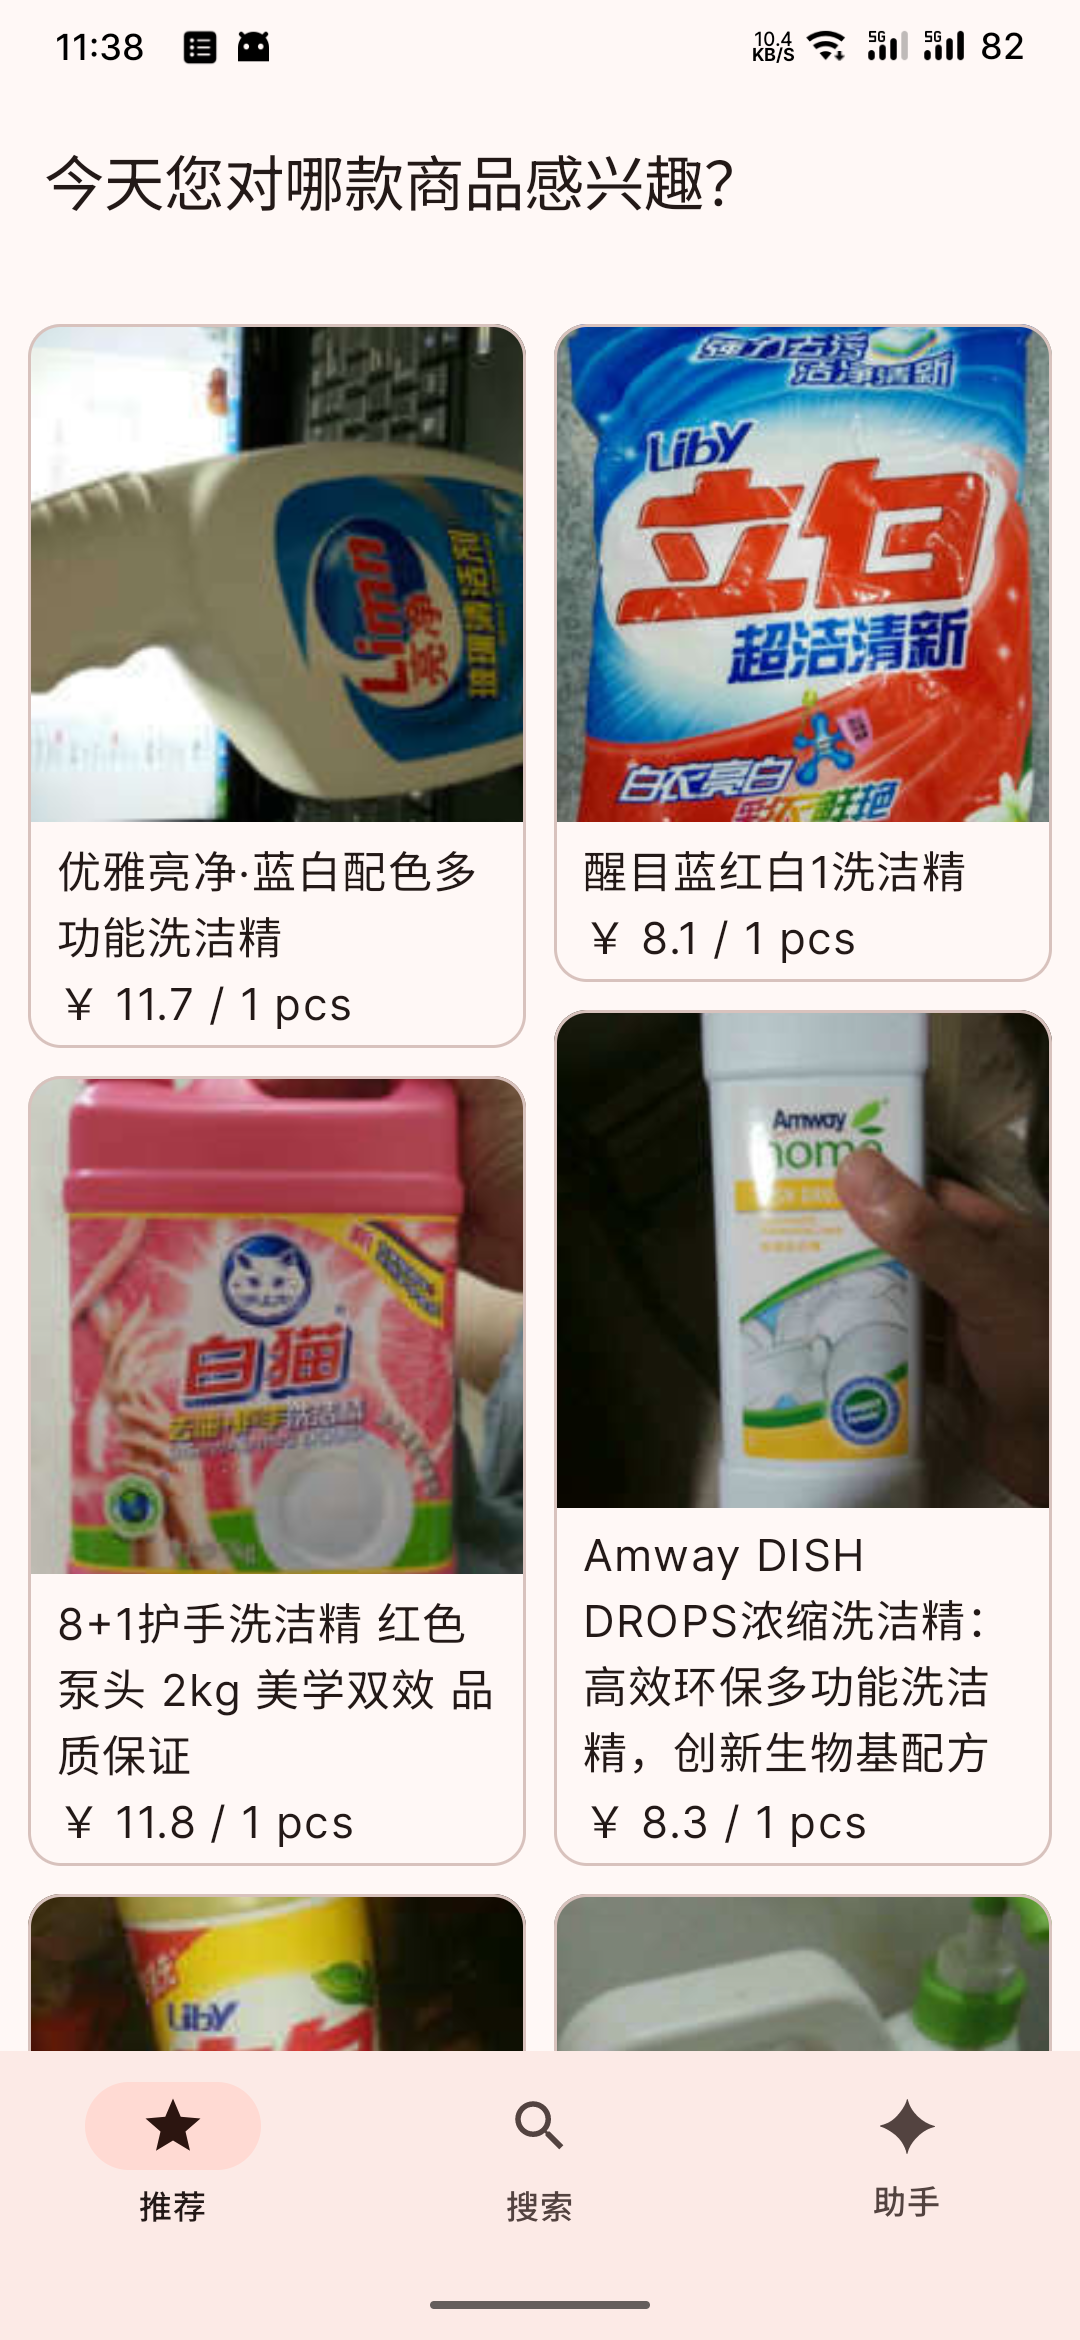
\includegraphics[width=0.3\textwidth]{./exp/seg-feat.png}}
    \hfill
    \subfloat{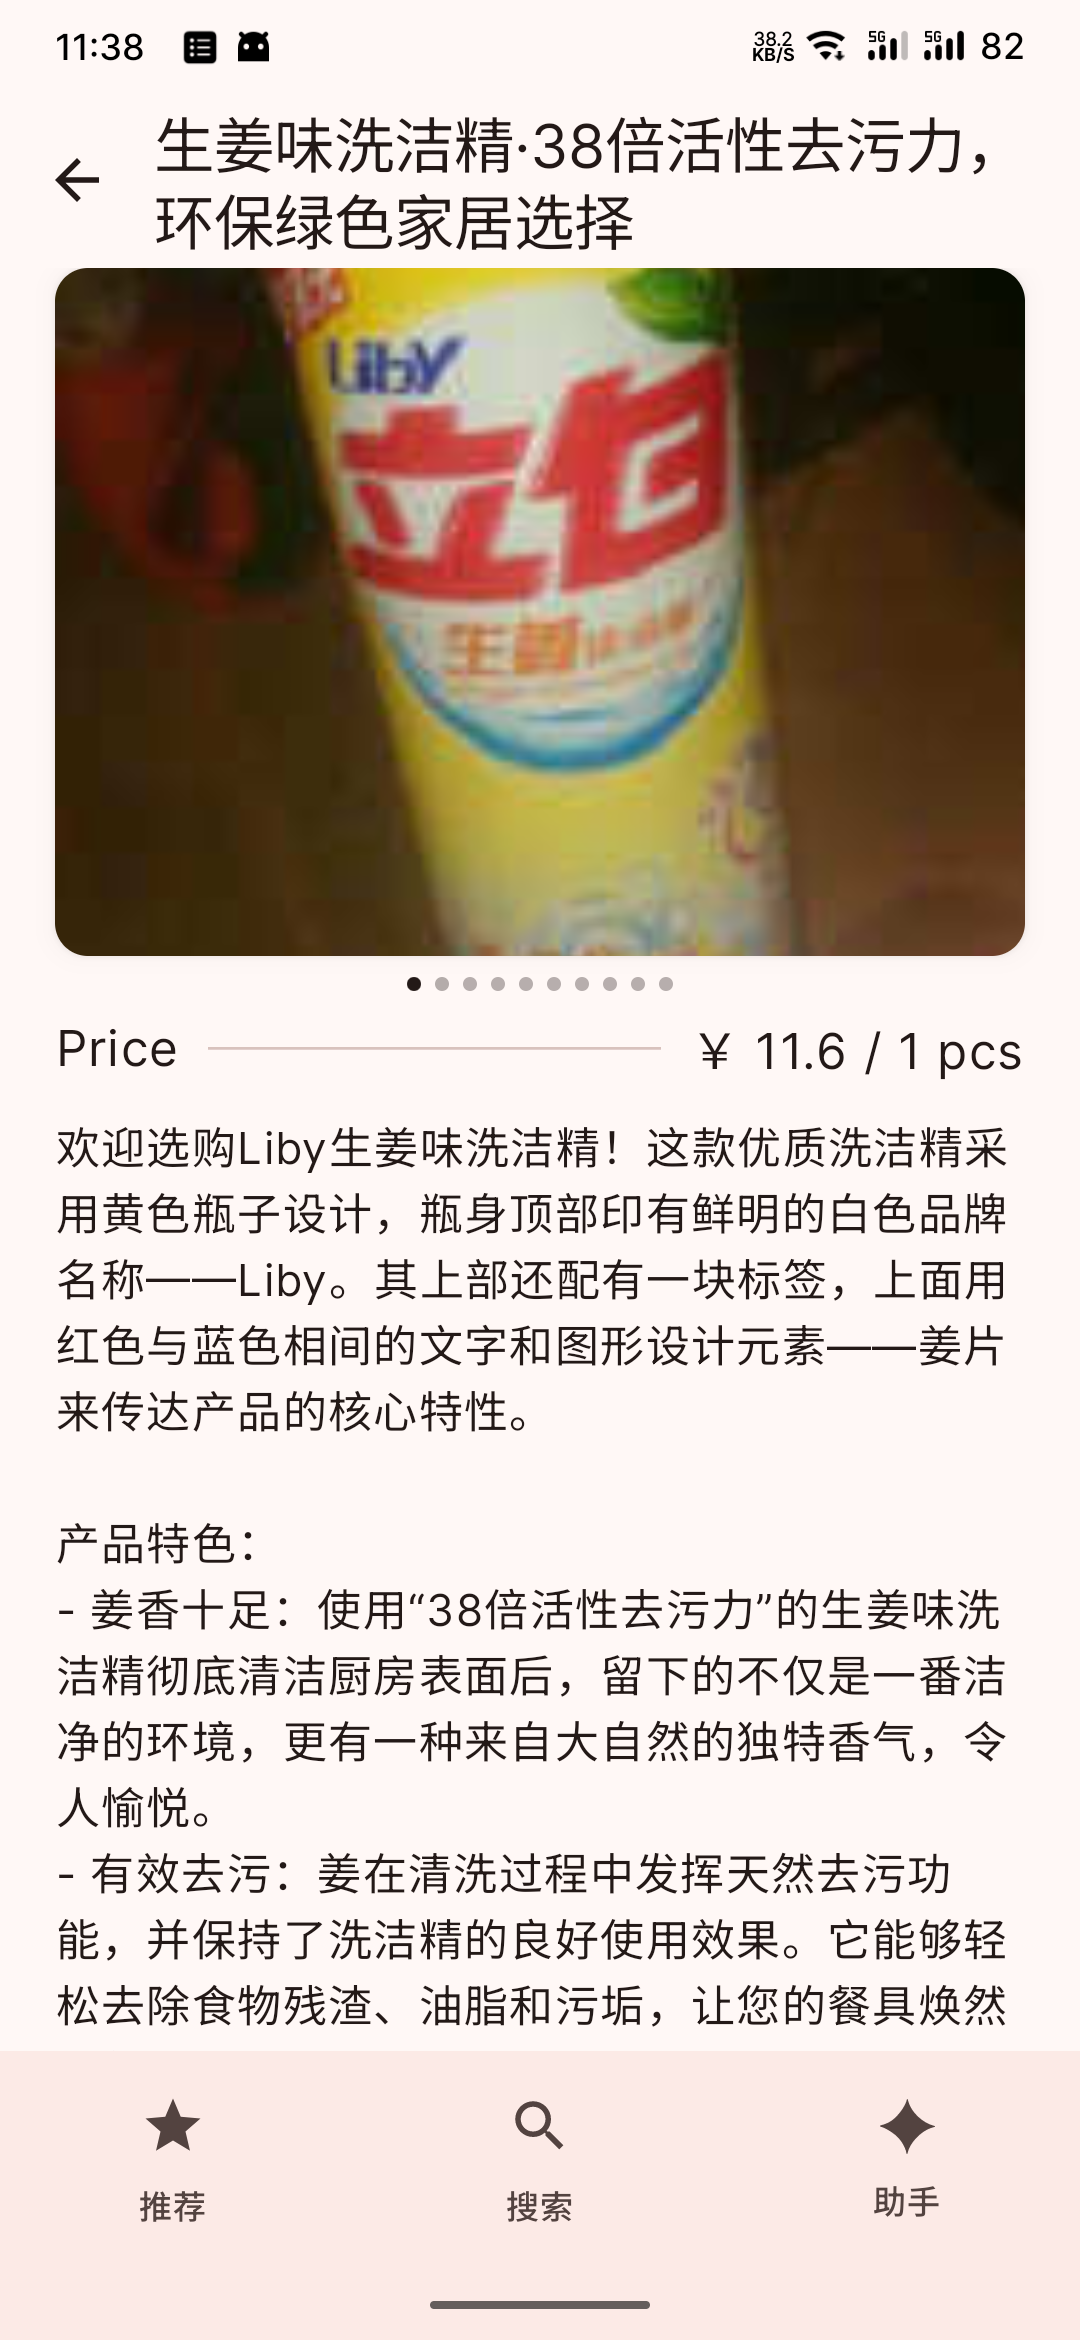
\includegraphics[width=0.3\textwidth]{./exp/seg-detail.png}}
	\caption{(todo)}
	\label{fig:seg-generic}
\end{figure}

\begin{figure}[htbp]
    \centering
    \subfloat{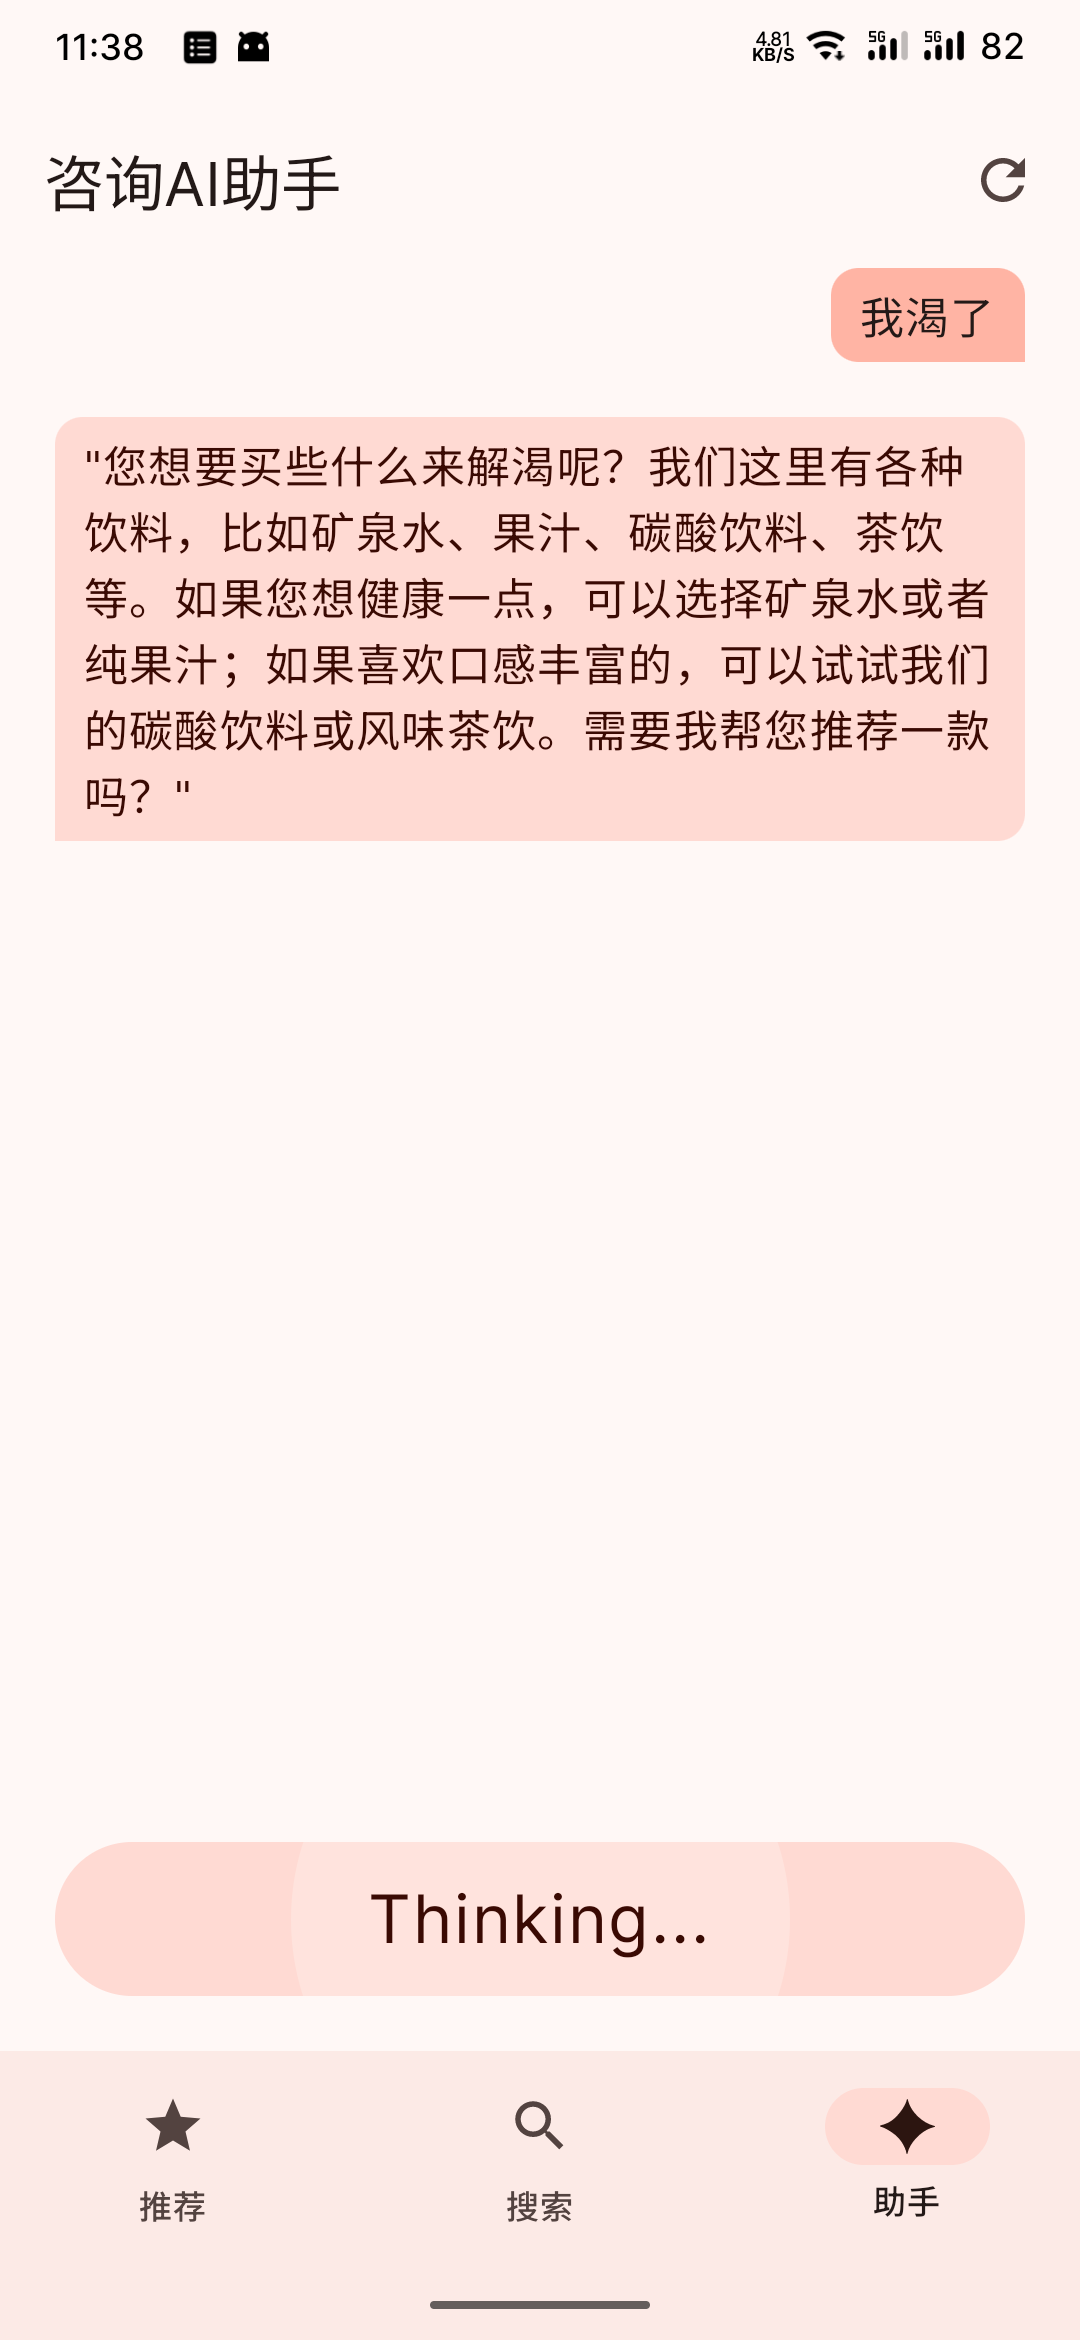
\includegraphics[width=0.33\textwidth]{./exp/seg-assist-1.png}}
    \hfill
    \subfloat{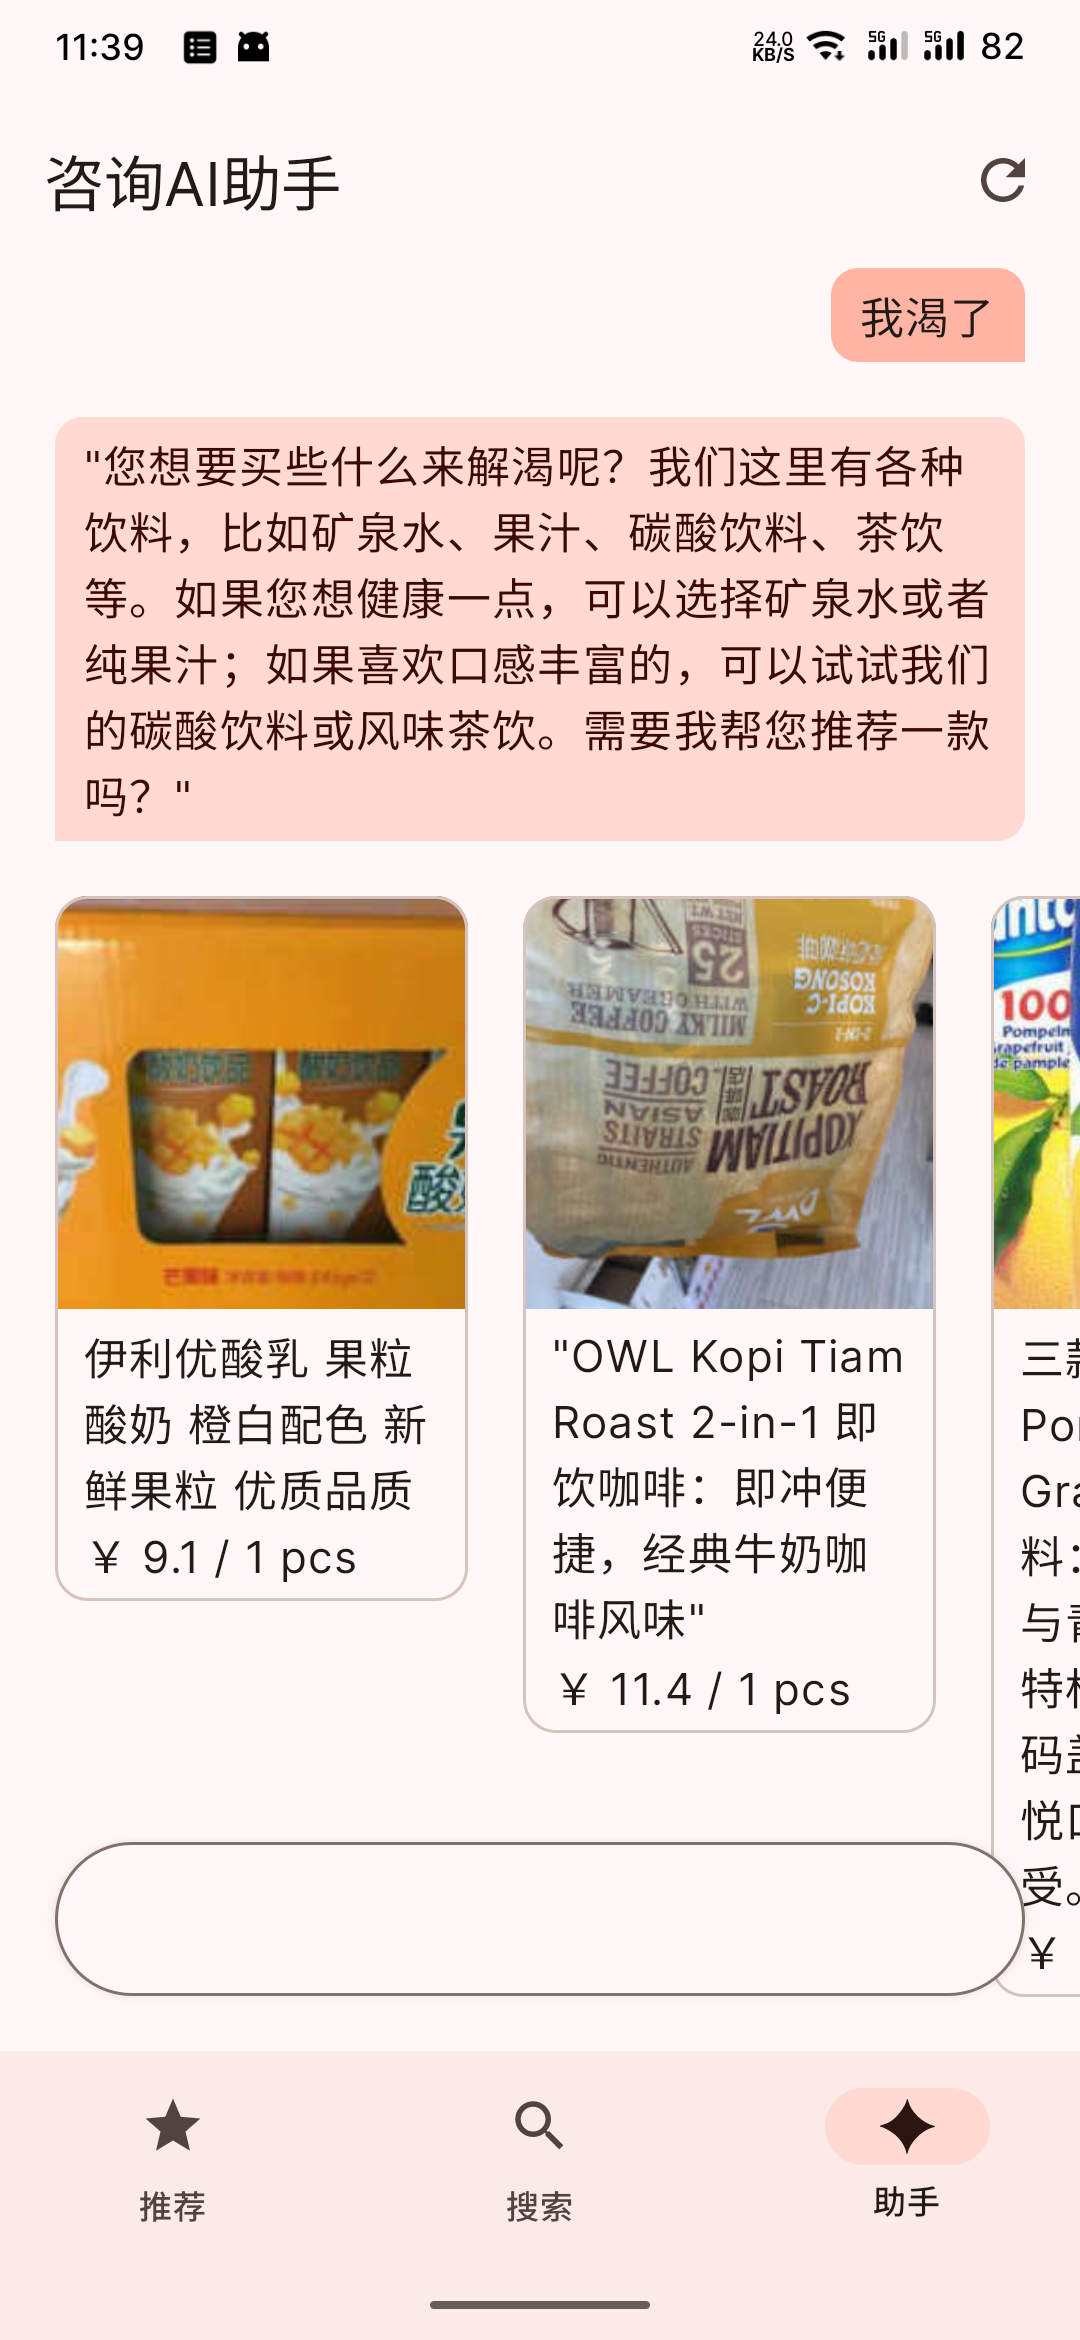
\includegraphics[width=0.33\textwidth]{./exp/seg-assist-2.png}}
	\caption{(todo)}
	\label{fig:seg-assist}
\end{figure}

\subsubsection{EasyCheckout}

\begin{figure}[htbp]
    \centering
    \subfloat{\includegraphics[width=0.45\textwidth]{./exp/ec-tare.png}}
    \hfill
    \subfloat{\includegraphics[width=0.45\textwidth]{./exp/ec-bc.png}}
    \vspace{1em}
    \subfloat{\includegraphics[width=0.45\textwidth]{./exp/ec-wr-1.png}}
    \hfill
    \subfloat{\includegraphics[width=0.45\textwidth]{./exp/ec-wr-2.png}}
	\caption{(todo)}
	\label{fig:ec}
\end{figure}